%%%%%% Run at command line, run
%%%%%% xelatex grad-sample.tex 
%%%%%% for a few times to generate the output pdf file
\documentclass[12pt,oneside,openright,a4paper]{cpe-english-project}


\usepackage{polyglossia}
 \setdefaultlanguage{english}
 \setotherlanguage{thai}
\newfontfamily\thaifont[Script=Thai,Scale=1.23]{TH Sarabun New}
\defaultfontfeatures{Mapping=tex-text,Scale=1.0,LetterSpace=0.0}
\setmainfont[Scale=1.0,LetterSpace=0,WordSpace=1.0,FakeStretch=1.0]{Times New Roman}
\emergencystretch=10pt
%\XeTeXlinebreaklocale "th_TH"	
%\XeTeXlinebreakskip = 0pt plus 1pt
%\setmathfont(Digits)[Scale=1.0,LetterSpace=0,FakeStretch=1.0]{Times New Roman}


%%%%%%%%%%%%%%%%%%%%%%%%%%%%%%%%%%%%%%%%%%%%%%%%%%%%%%%%%%%%%%%%%%%
% Customize below to suit your needs 
% The ones that are optional can be left blank. 
%%%%%%%%%%%%%%%%%%%%%%%%%%%%%%%%%%%%%%%%%%%%%%%%%%%%%%%%%%%%%%%%%%%
% First line of title
\def\disstitleone{Writing Aid to Avoid Repetitions}   
% Second line of title
%\def\disstitletwo{Project/Indep title line 2 (optional)}   
% Your first name and lastname
\def\dissauthor{Mr.Annop Pornsawatdipak}   % 1st member
%%% Put other group member names here ..
\def\dissauthortwo{Mr.Thanapatr Amnuaywit}   % 2nd member (optional)
\def\dissauthorthree{}   % 3rd member (optional)


% The degree that you're persuing..
\def\dissdegree{Bachelor of Engineering} % Name of the degree
\def\dissdegreeabrev{B.Eng} % Abbreviation of the degree
\def\dissyear{2022}                   % Year of submission
\def\thaidissyear{2565}               % Year of submission (B.E.)

%%%%%%%%%%%%%%%%%%%%%%%%%%%%%%%%%%%%%%%%%%%%
% Your project and independent study committee..
%%%%%%%%%%%%%%%%%%%%%%%%%%%%%%%%%%%%%%%%%%%%
\def\dissadvisor{Asst. Prof. Nuttanart Muansuwan, Ph.D.}  % Advisor
%%% Leave it empty if you have no Co-advisor
\def\disscoadvisor{}  % Co-advisor
\def\disscommitteetwo{Asst.Prof. Rajchawit Sarochawikasit}  % 3rd committee member (optional)
\def\disscommitteethree{Taweechai Nuntawisuttiwong, Ph.D.}   % 4th committee member (optional) 
\def\disscommitteefour{Piyanit Wepulanon, Ph.D.}    % 5th committee member (optional) 

\def\worktype{Project} %%  Project or Independent study
\def\disscredit{3}   %% 3 credits or 6 credits


\def\fieldofstudy{Computer Engineering} 
\def\department{Computer Engineering} 
\def\faculty{Engineering}

\def\thaifieldofstudy{วิศวกรรมคอมพิวเตอร์} 
\def\thaidepartment{วิศวกรรมคอมพิวเตอร์} 
\def\thaifaculty{วิศวกรรมศาสตร์}
 
\def\appendixnames{Appendix} %%% Appendices or Appendix

\def\thaiworktype{ปริญญานิพนธ์} %  Project or research project % 
\def\thaidisstitleone{โปรแกรมช่วยเขียนโดยหลีกเลี่ยงคำซ้ำ}
%\def\thaidisstitletwo{หัวข้อปริญญานิพนธ์บรรทัดสอง}
\def\thaidissauthor{นายอรรณพ พรสัวสดิภักดิ์}
\def\thaidissauthortwo{นายธนภัทร อำนวยวิทย์} %Optional
\def\thaidissauthorthree{} %Optional

\def\thaidissadvisor{ผศ.ดร.ณัฐนาถ เหมือนสุวรรณ}
%% Leave this empty if you have no co-advisor
\def\thaidisscoadvisor{} %Optional
\def\thaidissdegree{วิศวกรรมศาสตรบัณฑิต}

% Change the line spacing here...
\linespread{1.15}

%%%%%%%%%%%%%%%%%%%%%%%%%%%%%%%%%%%%%%%%%%%%%%%%%%%%%%%%%%%%%%%%
% End of personal customization.  Do not modify from this part 
% to \begin{document} unless you know what you are doing...
%%%%%%%%%%%%%%%%%%%%%%%%%%%%%%%%%%%%%%%%%%%%%%%%%%%%%%%%%%%%%%%%


%%%%%%%%%%%% Dissertation style %%%%%%%%%%%
%\linespread{1.6} % Double-spaced  
%%\oddsidemargin    0.5in
%%\evensidemargin   0.5in
%%%%%%%%%%%%%%%%%%%%%%%%%%%%%%%%%%%%%%%%%%%
%\renewcommand{\subfigtopskip}{10pt}
%\renewcommand{\subfigbottomskip}{-5pt} 
%\renewcommand{\subfigcapskip}{-6pt} %vertical space between caption
%                                    %and figure.
%\renewcommand{\subfigcapmargin}{0pt}

\renewcommand{\topfraction}{0.85}
\renewcommand{\textfraction}{0.1}

\newtheorem{theorem}{Theorem}
\newtheorem{lemma}{Lemma}
\newtheorem{corollary}{Corollary}

\def\QED{\mbox{\rule[0pt]{1.5ex}{1.5ex}}}
\def\proof{\noindent\hspace{2em}{\itshape Proof: }}
\def\endproof{\hspace*{\fill}~\QED\par\endtrivlist\unskip}
%\newenvironment{proof}{{\sc Proof:}}{~\hfill \blacksquare}
%% The hyperref package redefines the \appendix. This one 
%% is from the dissertation.cls
%\def\appendix#1{\iffirstappendix \appendixcover \firstappendixfalse \fi \chapter{#1}}
%\renewcommand{\arraystretch}{0.8}
%%%%%%%%%%%%%%%%%%%%%%%%%%%%%%%%%%%%%%%%%%%%%%%%%%%%%%%%%%%%%%%%
%%%%%%%%%%%%%%%%%%%%%%%%%%%%%%%%%%%%%%%%%%%%%%%%%%%%%%%%%%%%%%%%


\begin{document}
\pdfstringdefDisableCommands{%
\let\MakeUppercase\relax
}
\begin{center}
  
\includegraphics[width=2.8cm]{logo02.jpg}
\end{center}
\vspace*{-1cm}

\maketitlepage
\makesignaturepage 

%%%%%%%%%%%%%%%%%%%%%%%%%%%%%%%%%%%%%%%%%%%%%%%%%%%%%%%%%%%%%%
%%%%%%%%%%%%%%%%%%%%%% English abstract %%%%%%%%%%%%%%%%%%%%%%%
%%%%%%%%%%%%%%%%%%%%%%%%%%%%%%%%%%%%%%%%%%%%%%%%%%%%%%%%%%%%%%
\abstract

The computer-assisted writing aims to help improve the quality of a piece of text with the help of a computer. Most of the tools focus on fixing grammatical accuracy and misspelled words, only a few of them offer repetition detectors. In this project, we will be creating a program to keep track of the words and phrases' frequency. Moreover, our program will suggest alternative words that fit in the original context, thus, the writer can replace the word marked as repetitive with a new suggested word instead. Our proposed solutions consisted of two main parts, the detector, and the suggestor. In the first part, the program tries to detect only relevant repetitions and filter out very specific words or very trivial words. It can detect a single word (unigram) up to three words (trigram) repetitions. Next, the suggestor module will generate multiple substitution candidates by feeding the original sentence along with the masked sentence into the Transformer model. The models such as BERT and Roberta are trained with Masked Language Modelling, which we can use to predict the mask position, in this case, the target word to replace. The generated candidates will be evaluated by four different judges (judges = models), and the final result will be determined using a consensus-based ranking system to find broadly acceptable positions among all judges.

\begin{flushleft}
\begin{tabular*}{\textwidth}{@{}lp{0.8\textwidth}}
\textbf{Keywords}: & Overused word detector / repetitive word detector / BERT / NLP
\end{tabular*}
\end{flushleft}
\endabstract

%%%%%%%%%%%%%%%%%%%%%%%%%%%%%%%%%%%%%%%%%%%%%%%%%%%%%%%%%%%%%%
%%%%%%%%%% Thai abstract here %%%%%%%%%%%%%%%%%%%%%%%%%%%%%%%%%
%%%%%%%%%%%%%%%%%%%%%%%%%%%%%%%%%%%%%%%%%%%%%%%%%%%%%%%%%%%%%%
{
%\begin{thai}
\XeTeXlinebreaklocale "th_TH"	
\XeTeXlinebreakskip = 0pt plus 1pt
\thaifont
\thaiabstract

การเขียนโดยใช้คอมพิวเตอร์ช่วยมีจุดมุ่งหมายเพื่อช่วยปรับปรุงคุณภาพของข้อความด้วยความช่วยเหลือของคอมพิวเตอร์ เครื่องมือส่วนใหญ่มุ่งเน้นไปที่การแก้ไขความถูกต้องทางไวยากรณ์และคำที่สะกดผิด แต่ก็ยังมีเครื่องมือน้อยที่ใช้ในการตรวจจับคำซ้ำ ในโครงการนี้ เราจะสร้างโปรแกรมเพื่อติดตามความถี่ของคำและวลี นอกจากนี้ โปรแกรมของเราจะแนะนำคำทางเลือกที่เหมาะสมกับบริบทเดิม ดังนั้น ผู้เขียนสามารถแทนที่คำซ้ำด้วยคำใหม่ที่แนะนำแทน วิธีแก้ปัญหาที่เรานำเสนอประกอบด้วยสองส่วนหลัก ได้แก่ ส่วนตรวจจับ และส่วนแนะนำ ในส่วนแรก โปรแกรมจะพยายามตรวจหาเฉพาะคำซ้ำที่เกี่ยวข้องและกรองคำเฉพาะหรือคำที่ไม่สำคัญออก โปรแกรมของเราสามารถตรวจจับคำซ้ำได้ตั้งแต่คำเดียว (ยูนิแกรม) จนถึงสามคำ (ไตรแกรม) จากนั้นโมดูลผู้แนะนำจะสร้างรายการคำตัวเลือกโดยป้อนประโยคต้นฉบับพร้อมกับประโยคที่ทำการมาสก์โทเค่นลงในแบบจำลองทรานส์ฟอร์มเมอร์สเช่น เบิร์ทและ โรเบอร์ต้า ได้รับการฝึกฝนด้วย มาสก์แลงเกวจโมเดลลิ่ง ซึ่งเราสามารถใช้เพื่อทำนายตำแหน่งของมาสก์ ในกรณีนี้ คำเป้าหมายที่จะแทนที่ รายการคำที่สร้างขึ้นจะได้รับการประเมินโดยผู้ตัดสินที่แตกต่างกัน 4 คน (ผู้ตัดสินหมายถึงแบบจำลอง) และผลลัพธ์สุดท้ายจะถูกตัดสินโดยใช้ระบบการจัดอันดับตามฉันทามติเพื่อค้นหาการจัดอันดับที่เป็นที่ยอมรับจากผู้ตัดสินทั้งหมด

\begin{flushleft}
\begin{tabular*}{\textwidth}{@{}lp{0.8\textwidth}}
 & \\

\textbf{คำสำคัญ}: & การตรวจจับคำที่ใช้บ่อย / การตรวจจับคำซ้ำ / BERT / NLP
\end{tabular*}
\end{flushleft}
\endabstract
%\end{thai}
}

%%%%%%%%%%%%%%%%%%%%%%%%%%%%%%%%%%%%%%%%%%%%%%%%%%%%%%%%%%%%
%%%%%%%%%%%%%%%%%%%%%%% Acknowledgments %%%%%%%%%%%%%%%%%%%%
%%%%%%%%%%%%%%%%%%%%%%%%%%%%%%%%%%%%%%%%%%%%%%%%%%%%%%%%%%%%%
%\preface
%Thanks GOD for giving me strength to complete this long and boring AF project.
%
%Thanks to me that I keep being lazy everyday so I can enjoy my life more than writing texts. I always give reward to myself everyday by resting after doing nothing for the whole day.

%%%%%%%%%%%%%%%%%%%%%%%%%%%%%%%%%%%%%%%%%%%%%%%%%%%%%%%%%%%%%
%%%%%%%%%%%%%%%% ToC, List of figures/tables %%%%%%%%%%%%%%%%
%%%%%%%%%%%%%%%%%%%%%%%%%%%%%%%%%%%%%%%%%%%%%%%%%%%%%%%%%%%%%
% The three commands below automatically generate the table 
% of content, list of tables and list of figures
\tableofcontents                    
%\listoftables
\listoffigures                      

%%%%%%%%%%%%%%%%%%%%%%%%%%%%%%%%%%%%%%%%%%%%%%%%%%%%%%%%%%%%%%
%%%%%%%%%%%%%%%%%%%%% List of symbols page %%%%%%%%%%%%%%%%%%%
%%%%%%%%%%%%%%%%%%%%%%%%%%%%%%%%%%%%%%%%%%%%%%%%%%%%%%%%%%%%%%
% You have to add this manually..
%\listofsymbols
%\begin{flushleft}
%\begin{tabular}{@{}p{0.07\textwidth}p{0.7\textwidth}p{0.1\textwidth}}
%\textbf{SYMBOL}  & & \textbf{UNIT} \\[0.2cm]
%$\alpha$ & Test variable\hfill & m$^2$ \\
%$\lambda$ & Interarival rate\hfill &  jobs/second\\
%$\mu$ & Service rate\hfill & jobs/second\\
%\end{tabular}
%\end{flushleft}
%%%%%%%%%%%%%%%%%%%%%%%%%%%%%%%%%%%%%%%%%%%%%%%%%%%%%%%%%%%%%%
%%%%%%%%%%%%%%%%%%%%% List of vocabs & terms %%%%%%%%%%%%%%%%%
%%%%%%%%%%%%%%%%%%%%%%%%%%%%%%%%%%%%%%%%%%%%%%%%%%%%%%%%%%%%%%
% You also have to add this manually..
%\listofvocab
%\begin{flushleft}
%\begin{tabular}{@{}p{1in}@{=\extracolsep{0.5in}}l}
%ABC & Adaptive Bandwidth Control \\
%MANET & Mobile Ad Hoc Network 
%\end{tabular}
%\end{flushleft}

%\setlength{\parskip}{1.2mm}

%%%%%%%%%%%%%%%%%%%%%%%%%%%%%%%%%%%%%%%%%%%%%%%%%%%%%%%%%%%%%%%
%%%%%%%%%%%%%%%%%%%%%%%% Main body %%%%%%%%%%%%%%%%%%%%%%%%%%%%
%%%%%%%%%%%%%%%%%%%%%%%%%%%%%%%%%%%%%%%%%%%%%%%%%%%%%%%%%%%%%%%


\chapter{Introduction}

\section{Problem statement and Approach} 

Writing a long text such as an essay, or an academic report can be challenging, especially for non-native English speakers. One of the most common problems is the overuse of certain vocabulary, which can distract the readers and make the article less professional. With limited lexical resources, the writing may sound boring and can potentially weaken the message the writer wants to convey. Particularly in academic writing where the readers are highly educated, repetition is an undesirable trait and can be seen as disrespectful to the readers (Fosu, 2020\cite{a}). This project will focus on helping non-native users of English to reduce repetitions in their writing which will improve the overall quality of their work.

\section{Objectives}
To a standalone system detect overused words or phrases in writing and suggest alternatives based on context.

\section{Project Scope}
\begin{itemize}
\item Overused word detection for detecting high-frequency words in the document.
\item Word suggestion for recommending a substitution word that fits in the context.
\item Suggestion does not include grammatical corrections, such as verb tense, spelling, etc.
\item Supports English language only
\end{itemize}

\section{Project Schedule}
\noindent{\large\bf  Term 1}\\ \\
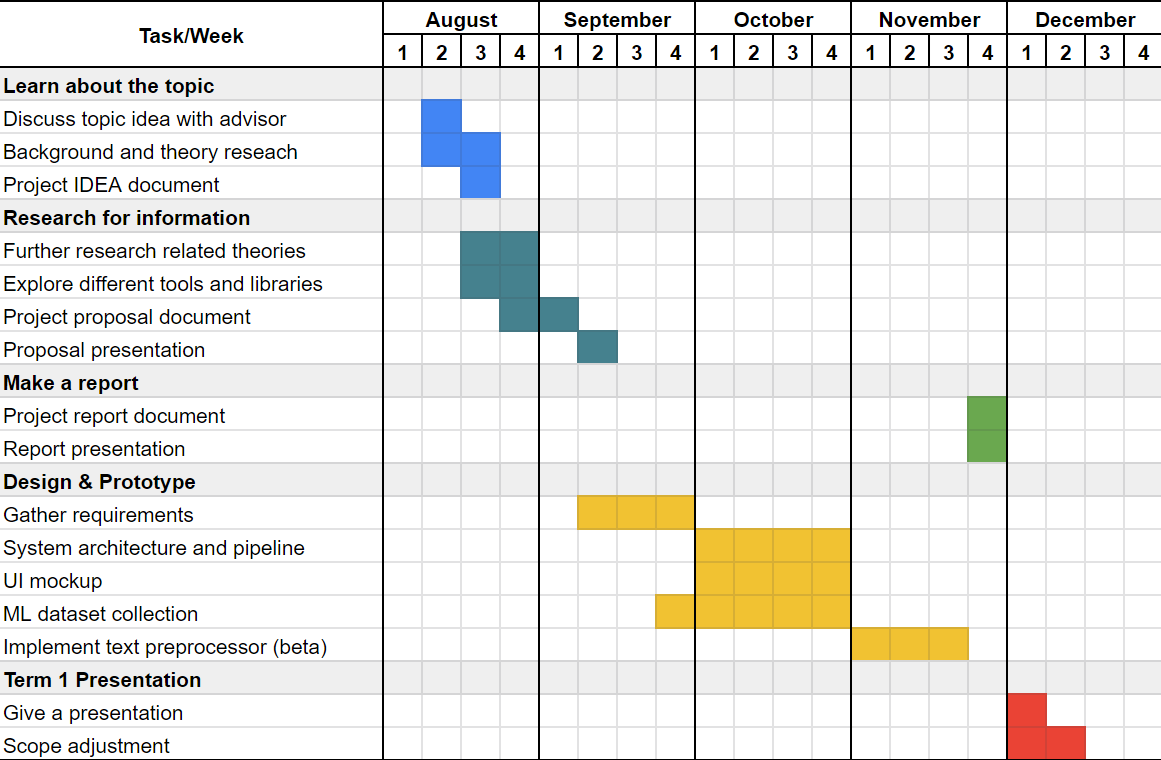
\includegraphics[width=15cm]{./img/chp1/schedule1.png}

\noindent{\large\bf  Term 2}\\ \\
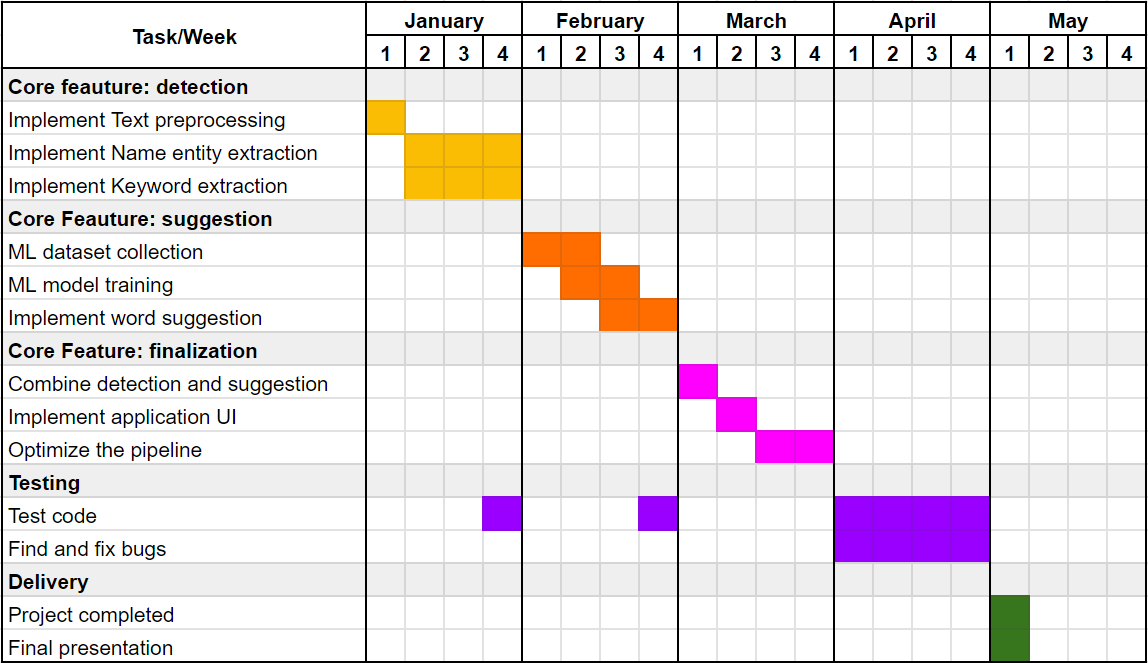
\includegraphics[width=15cm]{./img/chp1/schedule2.png}\\

Term 1\\
1. Learn about the topic
\begin{itemize}
\item Discuss topic idea
\item Define problem definition, scope and method
\item Make the IDEA document
\end{itemize}
2. Research for more information
\begin{itemize}
\item Further research related theories
\item Explore different tools and libraries
\item Make a final proposal and presentation   
\end{itemize} 
3. Design \& prototyping
\begin{itemize}
\item Gather requirements
\item Design system architecture and pipeline
\item Create an UI mockup
\item Try implementing text preprocessor
\end{itemize}
4. Term 1 final report and presentation\\


Term 2\\
1. Core feature: detection
\begin{itemize}
\item Implement Text Preprocessing
\item Implement Name Entity Extraction
\item Implement Keyword extraction
\end{itemize}
2. Core feature: suggestion
\begin{itemize}
\item Finish up ML datasets collecting process
\item ML model training
\item Implement word suggestion
\end{itemize}
3. Finalize the application
\begin{itemize}
\item Combine detection and suggestion
\item Optimize the pipeline
\item Implement application UI
\end{itemize}
4. Testing
\begin{itemize}
\item Application testing
\item Discover problems and errors
\item Fixing bugs
\end{itemize}
5. Delivery
\begin{itemize}
\item Complete the project
\item Final report and presentation
\end{itemize}


\section{Deliverables}
Term 1
\begin{enumerate}
\item Proposal
\item Project report(unfinished) and presentation
\item Requirement list
\item Text preprocessor (beta)
\item UI mockup
\item System architecture\\
\end{enumerate}

Term 2
\begin{enumerate}
\item Completed application
\item Completed project report
\end{enumerate}


%%%%%%%%%%%%%%%%%%%%%%%%%%%%%%%%%%%%%%%%%%%%%%%%%%%%%%%%%%%%
%%%%%%%%%%%%%%  Literature Review %%%%%%%%%%%%%%%%%%%%%%%%%%
%%%%%%%%%%%%%%%%%%%%%%%%%%%%%%%%%%%%%%%%%%%%%%%%%%%%%%%%%%%%
\chapter{Background Theory and Related Work}
\section{Background}
Writing an academic article in English poses a number of challenges to the writer, particularly those whose English is not their first language for example ESL students (English as Second Language) and EFL students (English as Foreign Language). There are a number of difficulties that often come up when writing a long piece of tex;t namely sentence structural problems, grammatical mistakes, coherence and cohesion. Nonetheless, one of the most prominent struggle writers face is having limited lexical resources which leads to the repetitive use of a certain word. The research regarding connector usage of Japanese EFL learners found that learners significantly overuse some connecting devices, especially sentence-initial positions. It also revealed that both native users and Japanese EFL students share a common set of high-frequency linking devices \cite{v}. The researchers suggested some of the reasons for this problem include the lack of familiarity with the word and inadequate knowledge. Another investigation \cite{w} supports the claim by pointing out a familiarity issue with certain connecting words which ultimately resulted in repetitive use of linking words. 

Repetition in an academic context is especially critical due to the audience being highly knowledgeable. As Fosu \cite{a} said, “Not only is repeating things distracting, but it’s also somewhat insulting to a person’s intelligence”. In certain scenarios, the issue arises due to the mindlessness of the writer rather than a lack of skill. As the text becomes longer, it is harder to keep track of how often a certain vocabulary has been used in the text, thus the repetition becomes more difficult to control. The writer can certainly read through the entire document to identify overuse words, however, this is a daunting task and time-consuming to re-read multiple times.

Natural Language Processing (NLP) has been greatly advanced in recent years both in terms of efficiency and accuracy. A state-of-art machine learning-based NLP has emerged thanks to tremendous textual data human generates each day. Currently, there are numerous services focused on computer-assited writing, for instance, Grammarly, Prowritingaid, Gramara, Microsoft Word’s Editor, Writer.com, and more. Most of them focus on fixing grammatical errors, typos, and punctuation, only a few of them offer overuse word detection. As mentioned above, we decided to create an application to help writers avoid repetition by keeping track of their word frequency as well as suggesting alternative words to use. The target user of this project is non-native English student writers in an academic context.
\section{Related Theory}
\subsection{Natural Language Processing}
Natural language Processing (NLP) is a sub-field of computer science (also a branch of Artificial intelligence depending on the technique used) defined as a way to give computers the ability to understand text and spoken language in the same way human beings can \cite{c}. According to IBM,  NLP is a multidisciplinary combining computational linguistics, rule-based modeling of human language, statistics, machine learning, and deep learning models. All of these enable computers to interpret natural language in both textual and verbal forms.  NLP has various use cases both for personal and business use such as machine translators, voice-activated speakers, virtual assistants, virtual agents, customer service chatbots, and social media analysis respectively. Early, NLP applications often rely on a rule-based approach which means the programmer must hard code all the linguistic rules to let the computer perform NLP tasks. However, human language is full of ambiguity and exceptions which makes traditional methods cannot scale to capture all the nuance of everchanging human language. Thus, most modern-day NLP applications let the computer learn patterns by themself using Machine Learning instead.
\subsubsection{Part-of-speech Tagging}
A process of assigning the part of speech to different words in a piece of text. Part of speech is critical as some words can be both verb and noun depending on the usage for example “ship” in the product has been shipped or “ship” in the ship will not float. Conventionally, the POS tag uses hard-coded, rule-based approaches. However, with the advancement of technology, nowadays, machine learning techniques have become a standard for assigning part of speech to words in a sentence. This modern approach uses a statistical model trained on large multi-language datasets, it is capable of generalizing across all languages.

\subsubsection{Word sense disambiguation}
A method to determine which meaning to use in a certain context in case the word has more than one meaning. For example, “park” could mean a large public green area or bring a vehicle to a halt and leave it temporarily. This can be done through semantic analysis.

\subsubsection{Name entity recognition}
A technique used to automatically identify name and location in the given text, for instance, Steve Jobs was kicked out of Apple, here, Steve Jobs is a person, and Apple is a company.

\subsubsection{Sentiment analysis}
An attempt to interpret the tone and attitude of the text. Useful for detecting emotions, sarcasm, confusion, and suspicion in the text.

\subsubsection{Natural Language Generation}
A process where computers create textual information that humans can understand. A well-known example is OpenAI’s Generative Pretrained Transformer (GPT) which has taken the world by storm recently due to its human-like response. 


\subsubsection{Keyword Extraction}
A method used to automatically find the most relevant words and phrases from a piece of document \cite{f}. Allowing the computer to know the main idea of the text. Some of the most well-known techniques are KeyBERT, Rapid Automatic Keyword Extraction (aka. Rake), Yet Another Keyword Extractor (aka. YAKE), and TextRank.

\subsection{Pointwise Mutual Information}
Pointwise Mutual Information (PMI) is a technique used to analyze the association between words. PMI asks how much more the two words co-occur in our corpus than we would have a prior expected them to appear by chance \cite{e}. PMI permits the ability to detect word pairs that occur together, thus, is useful when performing a cooccurrence analysis of words in the corpus. The formula is as follows.

\subsection{Likelihood ratio}
	 Likelihood ratio or log-likelihood ratio is a measure of how two events are unlikely to be independent but occur together more than by chance. This is used to measure the level of association between tokens, aka. bigram, trigram. A higher score indicates a significant co-occurrence between those tokens. Unlike PMI, this metric is not biased toward low-frequency words.

\subsection{Byte-pair encoding (BPE)}
A type of tokenizer where the word is broken down into tokens each containing a single character. A token can be merged to form a larger group. Similarly, each group can also be joined together to form a word. Example: This is tokenizing → T h i s i s t o k e n i z i n g → th is to ke ni zi ng → this is token in zi ng. The most frequent character pair are merged into one token, which will be added to the vocabulary.  The process repeats until it the target vocabulary limit is reached.
The BPE-based tokenizer is used in multiple models including BERT and Roberta to combat the out-of-vocabulary problem. Considering the size and amount of datasets required to train the model, it  may encounter domain-specific vocabularies that are not in the dictionary.
A Wordpiece tokenizer is used in BERT family model. According to Eram M \cite{x},Instead of relying on the frequency of the pairs, WordPiece chooses the one which maximizes the likelihood of the training data. This means that it trains a language model starting on the base vocabulary and picks the pair with the highest likelihood. For example, Internationalization
→ inter national \#\#iz\#\#ation. This is again, to overcome the out-of-vocabulary problem.




\subsection{Attention}
Traditional sequence to sequence approaches such as LSTM and RNN tend to suffer from the vanishing gradient problem, where the model failed to capture long term dependencies in a lengthy text. The attention model comes to solve this problem as it permits the model to focus on only the important information of the input\cite{p}. Instead of encoding the entire input sentence into a fixed-sized vector, the model learned to attend to parts of the sentence that are relevant to the output it will produce.  The decoder performs additional before outputting the result which is 1) look at each hidden state received from the encoder, 2) assign each of them a score, 3) apply softmax to each score, thus, higher scores will be amplified, the lower scores will be suppressed.

\subsection{Transformer}
According to the paper called “Attention is all you need”, published in 2017 \cite{p}, the author purposed an encoder-decoder architecture based on attention layers which was later known as the transformer \cite{m}\cite{n}. Initially, the transformer is intended to be used in the translation field, but due to its performance, scalability and versatility, this method is widely adopted by the research community and enterprise to solve challenging NLP tasks. Unlike LSTM or RNN, where it can only process words in a sentence sequentially as dictated by the design. The encoder-decoder architecture processes input in parallel manners. 

\subsubsection{Input Embedding (1)}
Textual input must be converted into a vector or in NLP, we called it an embedding. Every word is represented as a vector of values corresponding to its meanings. 

\subsubsection{Positional Encoding (2)}
Due to its parallelism property, each word in a sentence will get through the model simultaneously which means it doesn't know what order they are in. The positional encoding assigns each embedding a vector denoting its position.

\subsubsection{Multi-headed attention (3)}
This mechanism allows the model to pay attention to a specific token in the input. The attention vector captures the relationship between each word to the other words in the sentence. In self-attention, the model will give more weight to itself. However, this is not ideal because we are interested in obtaining the interaction between words. So instead, there are multiple attention heads per word which will be averaged out to get the final attention vector for every word.

\subsubsection{Add and Norm (4)}
Normalization is performed on each output layer-wise.

\subsubsection{Feed Forward (5)}
A feed-forward neural network is applied to every attention vector. This will transform the attention vector into a suitable format for the decoder/encoder block. All the vectors are passed to the network parallelly.

\subsubsection{Masked multi-headed attention (6)}
The multi-headed attention block generates attention vectors for every word in the sentence and the take average to get the final attention vector denotes the relationship between words. This resembles multi-headed attention but now included masks.
The reason is to prevent the model from having access to the future token that has not appeared yet in the natural ordering of the sentence. Mask is essentially to replace those positions with zero. Thus, the attention score will be computed in accordance with the previous token only and not the future one. 

\subsubsection{Multi-head attention (7)}
The attention vectors and the vector from the encoder are passed to the block similar to the previous one except now the input is coming from the encoder. So, we may refer to it as an encoder-decoder attention block. This block contains vectors for both languages and this is where the mapping between the 2 languages takes place. The output is in a form of attention vectors representing the relationship of words from both languages. 

\subsubsection{Linear (8)}
A kind of feed-forward network expands the multi-headed attention output to the dimension of size equal to the vocabulary in the target language. 

\subsubsection{Softmax (9)}
Calculate the probability score ranging from 0 to 1 for every class (words in the language). The class with the highest probability will be selected as the final output.

\subsubsection{Masked langauge modelling}
A training objective used in Transformer models like BERT \cite{j} and Roberta \cite{u}. This technique masks some portions of the input sentence, the model will try to fill in the blank by looking at the remaining unmasked token. For example: 
In reality, rich people can bribe the officer to avoid a long prison sentence.
In reality, rich <mask> can bribe the officer to avoid a long prison sentence.
The model will try to predict what word would fit in the mask position taking into account the surrounding contexts. The model has been trained on huge datasets both online and offline sources such as Wikipedia text and book corpus. Despite enormous data, the model may give biased results toward a certain gender or race.
This technique combined with attention mechanism permits the model to learn and capture contextual information. Some of the models that utilize this technique are BERT, Roberta, XLM, and distilBert. There are many use cases namely, text summarization, question answering, translation, token classification, entailment problem, and more.


\subsubsection{Finetuning}
A machine learning technique used to adapt a pre-trained model to perform specialized tasks. For instance, ResNet, an image classification model has already gained some general knowledge about the visual world. When building a new model for a domain-specific problem, we do not need to train it from scratch, instead, we build on top of the pre-trained model. In this project, we experimented with this technique but the result was unsatisfactory. 

\subsubsection{Consensus Ranking}
A consensus-based ranking is a type of voting system used in an election. Instead of relying on a majority vote, consensus voting uses a broadly accepted preferential order to determine the winner\cite{y}. There are numerous existing policies, but in this project, the Borda count method will be adapted. Borda count is a family of positional voting first purposed by Nicholas of Cusa in 1435, the nomenclature “Borda” is named after the French mathematician and engineer Jean-Charles de Borda in 1770. Generally, voters will rank their most wanted candidate first, second, third, and so on. Each position is assigned a point, the first position gets n-1 point, and the last position gets 0 points (*where n is the number of candidates). The one who possessed the most points will be the winner.



\section{Technologies and Development Tools}
\subsection{Python} 
Python is an object-oriented programming language that supports a wide selection of libraries including PyTorch, Spacy, NLTK, etc. 
 
\subsection{PyTorch} 
A machine learning library written in python.

\subsection{Pycharm Community} 
Another code editing software from JetBrains, it’s an open source version, specialized on edit and testing code in Python language. 

\subsection{Natural Language Toolkit (NLTK)} 
A toolkit provides some of the basic operations in NLP including stemming, tokenization, cooccurrence analysis, etc. 

\subsection{Spacy} 
A more advanced NLP library shipped with several ready-to-use tools such as tokenizer, NER, POS, Lemmatizer, and Training pipeline.  

\subsection{Tkinter} 
A GUI builder for Python applications. Provide basic tools to create GUI elements such as a window, a button, an input field, etc. 

\subsection{Visual Studio Code} 
A code editing software from Microsoft. Supports a wide range of plugins and add-ons which help streamline the development process. Collaborative code editing allows teammates to work on the same project remotely anytime anywhere. 

\subsection{Matplotlib} 
A library to help visualize results as a graphical representation such as confusion matrix, correlation plot, performance analysis, etc. 



\subsection{Huggingface Transformer} 
An open-source library dedicated to the development of NLP applications using transformers. It is compatible with both Tensorflow and PyTorch. The package includes numerous state-of-the-art models including BERT, Roberta, XLNet, T5, and more. It also supports various NLP pipelines for performing different tasks out-of-the-box some of them are audio classification, question answering, summarization, and translation. Moreover, this library provides a range of utility functions for training, finetuning, inferencing, etc.

\subsection{Sentence Transformer} 
A library leveraging on the original BERT architecture and Huggingface’s Transformers library, provides the ability to work with sentence-level as opposed to token-level embedding in the vanilla BERT. The pre-trained models have been trained on the datasets including Standford Natural Language Inference (SNLI) containing 570K sentence pairs and Multi-Genre Natural Language Inference (MNLI) containing 430K pairs. The dataset is labeled with 3 tags namely contradiction, neutral, and entailment. The model will learn to classify each sentence into one of the three categories. The main goal of Sentence Transformer framework is to compute the semantic textual similarity between 2 sentences, semantic search, and paraphrase mining \cite{z}. The closeness of embeddings is assessed with a cosine similarity score. In our project, it will be used to evaluate the quality substitution candidates and determine their appropriate ranking.

\section{Related Research}
\subsection{Embedding Dropout}
As mentioned, BERT has been trained using masked language modeling, it is capable of predicting a masked token of the sentence. However, if we feed the sentence where a word is replaced with <masked> token, the predicted token will likely fit in the context but may not retain its original meaning. According to Zhou, et al.\cite{k}\cite{o}, the embedding dropout can be used to overcome this issue. It is the technique where the random index of the token will be set to zero, thus, it allows the model to get partial information about the target word but help avoid overfitting. This approach helps improve the performance of the prediction according to the researcher. Further evaluation of performance when implemented in our project is needed.

\subsection{Sentence Concatenation}
According to the article, A simple BERT-Based Approach for Lexical Simplification purposed by Jipeng et al \cite{l}. The research focuses on simplifying complex words, although not directly related, this method is applicable to our project. The authors state that considering the complex word w in sentence S, the word w is masked to create a new sentence S’ and feed into the model. By doing this, the model will not consider the influence of the complex word. To give some clue about the target word, the sentence with a masked token will be concatenated with the original sentence that has no mask. Both sentences are then passed into the model to get the prediction. This allows the model to get some contexts about the target words, therefore, the output will be relatively close to the target word. The sentence Concatenation technique guarded inappropriate predictions produced by the model. This behavior is expected because the model has been trained to guess the <mask> with the most probable word based on the context. However, in reality, the highest probability word although grammatically correct and perfectly make sense is not guaranteed to retain the sentence’s original meaning. 

\subsection{BERT}
Based on Bidirectional Encoder Representations from Transformer (aka. BERT), A machine learning-based approach purposed by Google AI Language \cite{d}. It achieved superior performance by reading the entire sequence of words at once, instead of left to right or right to left like most of the previous works. This allows the model to learn the context of words using clues from their surroundings. BERT has been trained using 2 objectives in mind\cite{j}. The first is called next-sentence prediction where it tries to predict whether the given sentence will follow the previous sentence or not. Next, the masked language model where the random part of the corpus is masked and the model tries to fill in the gap. This research has become one of the best-performing approaches in the NLP world. Despite that, the model itself is inefficient and slow to run due to the complexity, so in this project, we decided to use another model named Roberta. At its core, Roberta is similar to BERT but without the Next sentence prediction objective.
Roberta stands for A Robustly Optimized BERT Pretraining Approach proposed by Yinhan Liu et.al. This model includes some tweaks mainly in the masking technique, as a result, it performs better than the original BERT. The researcher used dynamic masking to change the masking pattern of the sentence in each epoch. Unlike in BERT where the masking is done only once at the beginning, thus it remains static throughout the procedure. The modified BERT also used larger batch sizes and datasets during the training. Allowing the model to advance even further. 

\subsection{Existing product in the market}

\subsubsection{Grammarly} 
A writing assistant powered by Artificial Intelligence based in San Francisco, California. Grammarly is a powerful tool that can suggest and correct written text in multiple dimensions, for instance, grammatical accuracy, plagiarism, tone detection, style guide, structural, and brand tone. It supports a variety of platforms including Microsoft Word, Google Docs, Mac, Windows, Chrome, Safari, Firefox, iPhone, iPad, and Grammarly Keyboard. According to its official website,  it generates over 350,000 suggestions every minute for its 30 million daily users (Grammarly, n.d.). Despite all the capabilities, besides grammar and spelling checker, most of the advanced features are not available on the free version, thus, the users must pay a monthly subscription to access them. Moreover, Grammarly doesn’t have any feature that focuses on the problem of repetition, so there is a gap to improve upon\cite{h}. 
\subsubsection{Prowritingaid.com} Another writing assistant tool claims its superiority, saying “good writing is bout more than just grammar”(ProWritingAid, n.d.). The tool highlights a range of writing issues including overused words, sentence structure, punctuation issues, repeated phrases, consistency, pacing, and readability. In terms of pricing, similar to Grammarly, ProWritingAid free offers basic functionality such as a spelling checker and basic grammar correction, other features are limited to paid users only. One interesting feature is the repeated words report, it summarizes all the most frequent words and gives some suggested alternatives to choose from. This feature detects repeated words and phrases spanning across the specified distance, for example, the distance of 300, any repeats beyond 300 characters apart will not be flagged\cite{g}. 

\subsubsection{Writer.com} Another writing assistant that can help polish a piece of writing. But it emphasizes on team editing and content creation for the brand. There are numerous features that are far beyond the scope of the 2 previously mentioned services, such as a customized machine learning model using a custom writing style, and collaborative writing in real time that ensure consistency across all the team members. The basic corrections are available in its free plan, but any advanced features require a subscription\cite{i}.

 
\begin{figure}[!h]\centering
\setlength{\fboxrule}{0.2mm} % can define this in the preamble
\setlength{\fboxsep}{1cm}
\fbox{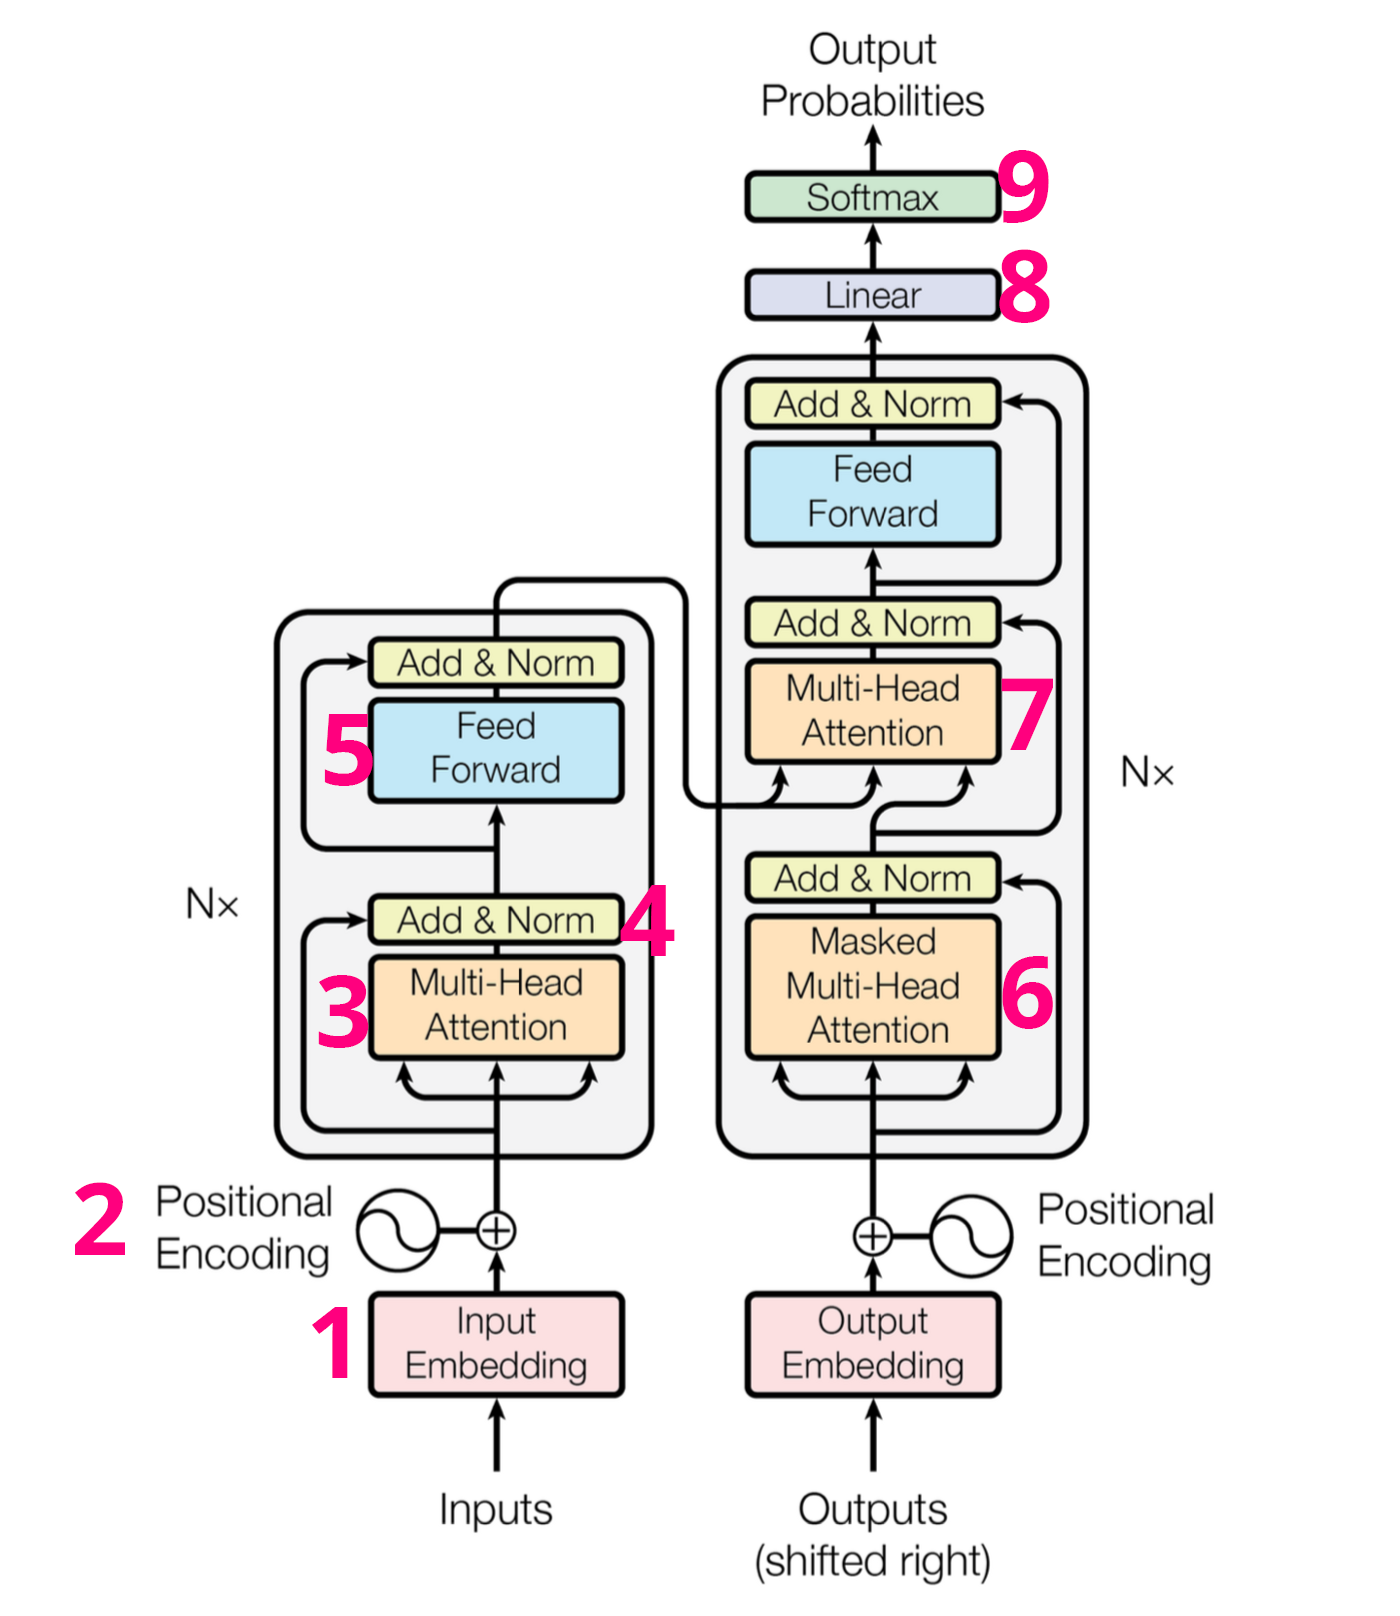
\includegraphics[width=15cm]{./img/chp2/transformerLables.png}}
\caption{The network model of Transformer architecture}\label{fig:model2}
\end{figure}


\chapter{CHAPTER 3 DESIGN AND METHODOLOGY}
In this chapter, we will be discussing the design of each component in our program, how an individual module works, and how they work together to perform a certain task.

\section{System Architecture}
\begin{figure}[!h]\centering
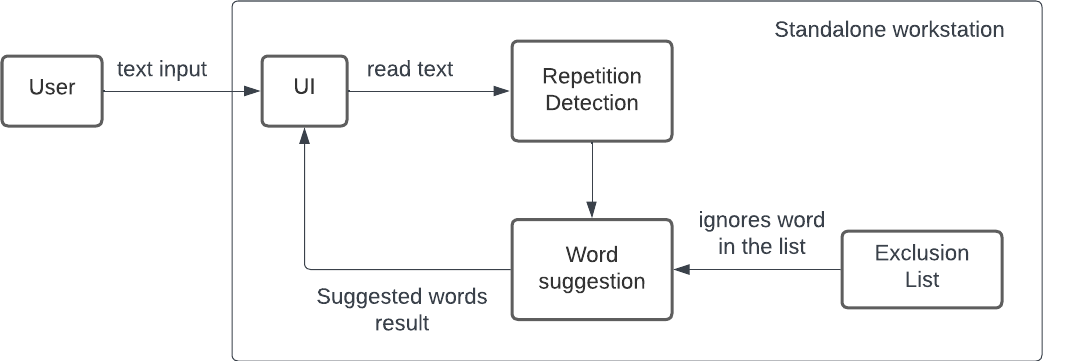
\includegraphics[width=15cm]{./img/chp3/SysArch.png}
\caption{System Architecture of an application}\label{fig:sysarch}
\end{figure}

Figure \ref{fig:sysarch} shows an application architecture in a diagram. The system is a standalone program, There’s basically just user interaction with the application side, and some general process of repetition search and word suggestion logic. After the user inputs text by typing and/or importing from other sources by copy and paste the text into the application text input area. The program will read those texts and start a repetition search by counting word occurrences.  After searching, the text data will be sent to another software’s part which is the word suggestion part, working along with a trained text model. And return matched words excluded from the exclusion list given from the user, that can be replaced with those repetition whether it has or not.

\section{Feature Lists} \label{sec:featlist}

\subsection{Editor}
	Our program’s basic function is to allow users to type in texts or paste them from other sources, so the program can use these texts with other functions.

\subsection{Repetition highlights} \label{subsec:rephigh}
	As the name said. The program should highlight the repetitions for the entire text input that user gives, and to not let the user get dazzled when seeing those repetitions in case there are many repeated words in the document. Only the first word or every repetition word will be highlighted, and only shows all the repetition locations when the user hovers or clicks on it.
\subsection{Repetition replacement suggestion}

	When a user clicks on any repetition words found, a list of similar or the word that can be replaced will be shown on the UI for the user to make a decision.
\subsection{Word exception list}
	In case that user doesn’t want this specific word to be detected as a repetition whether in this document or others. They can select the word as an exception. And this list of exceptions can be decided to use in other documents, use for individual words, or not used at all.

\section{Use case Diagram and Sequence Diagram}

\subsection{Use case diagram}
\begin{figure}[!h]\centering
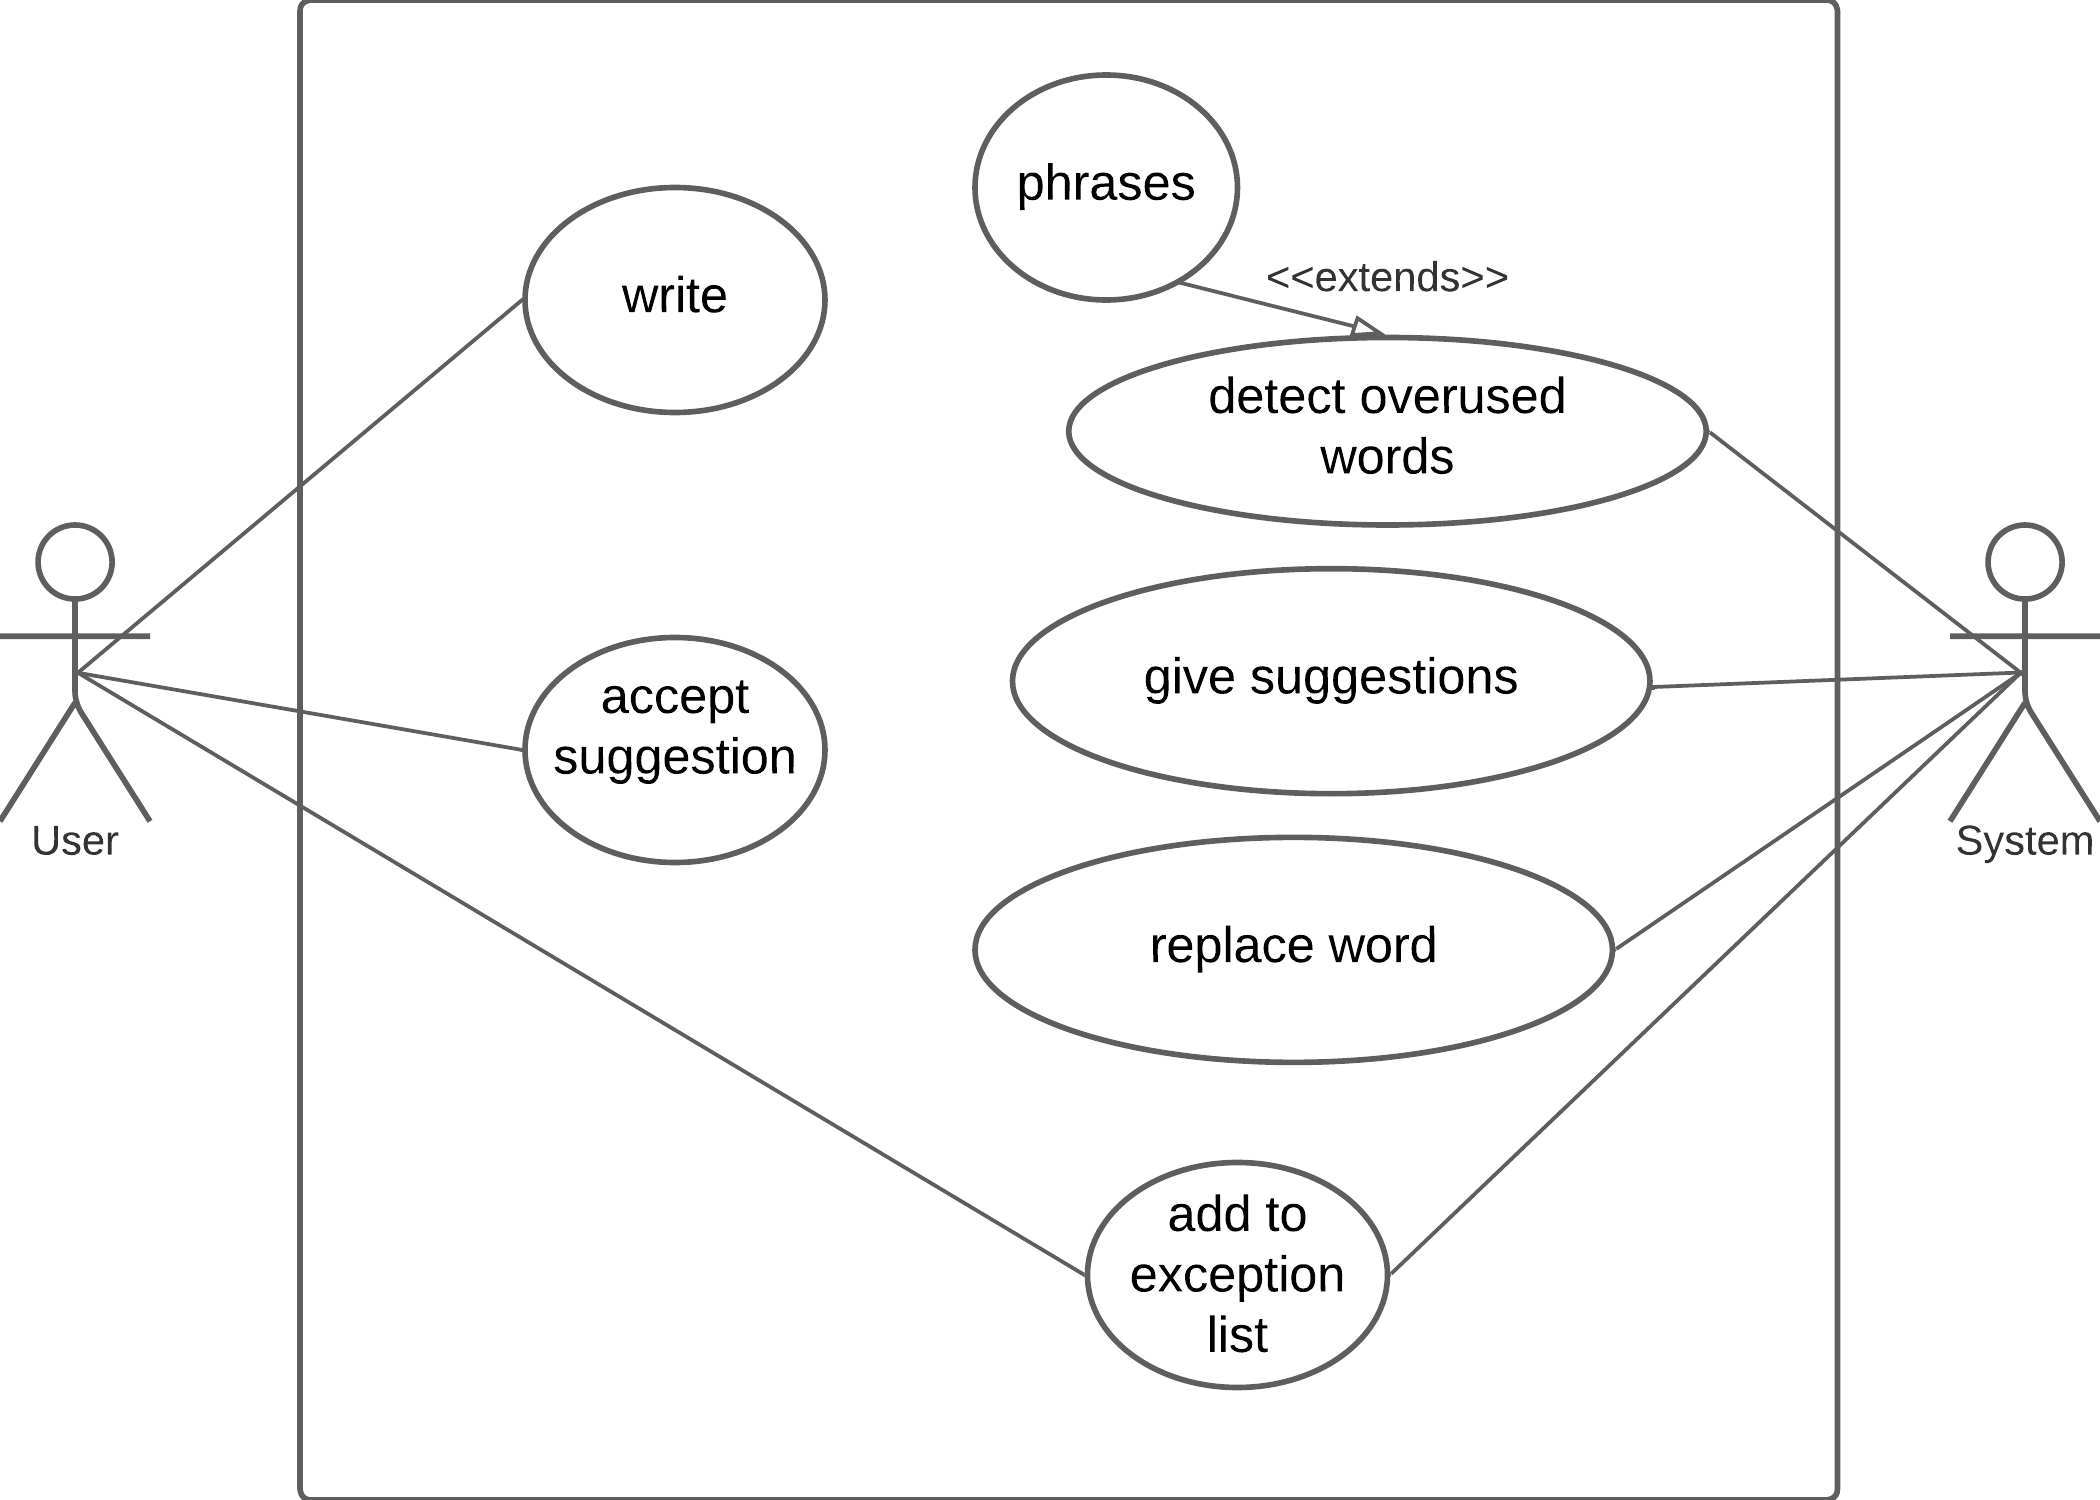
\includegraphics[width=15cm]{./img/chp3/Usecase.png}
\caption{Overview Use case Diagram}\label{fig:usecase}
\end{figure}

Figure \ref{fig:usecase} displays all use cases and actors who interact with them. The diagram shows all of the main goals that the program should support in each use case.

\begin{enumerate}
\item Writing texts into the program, either by typing in directly or copy and pasting text.
\item Detecting overused words or phrases in the text given.
\item Giving suggestions of a replacement word to the user.
\item Accepting the suggestion, so the suggestion word can be used to replace in the text.
\item Rejecting the suggestion, so that overused words will be ignored.
\item Add overused words to the exception list which will not be suggested later on the document.
\item Replacing the suggestion word to where overused words are.
\end{enumerate}

\subsection{Sequence diagram}
\noindent{\large\bf  Scenario 1: User input texts into the program}
\begin{figure}[!h]\centering
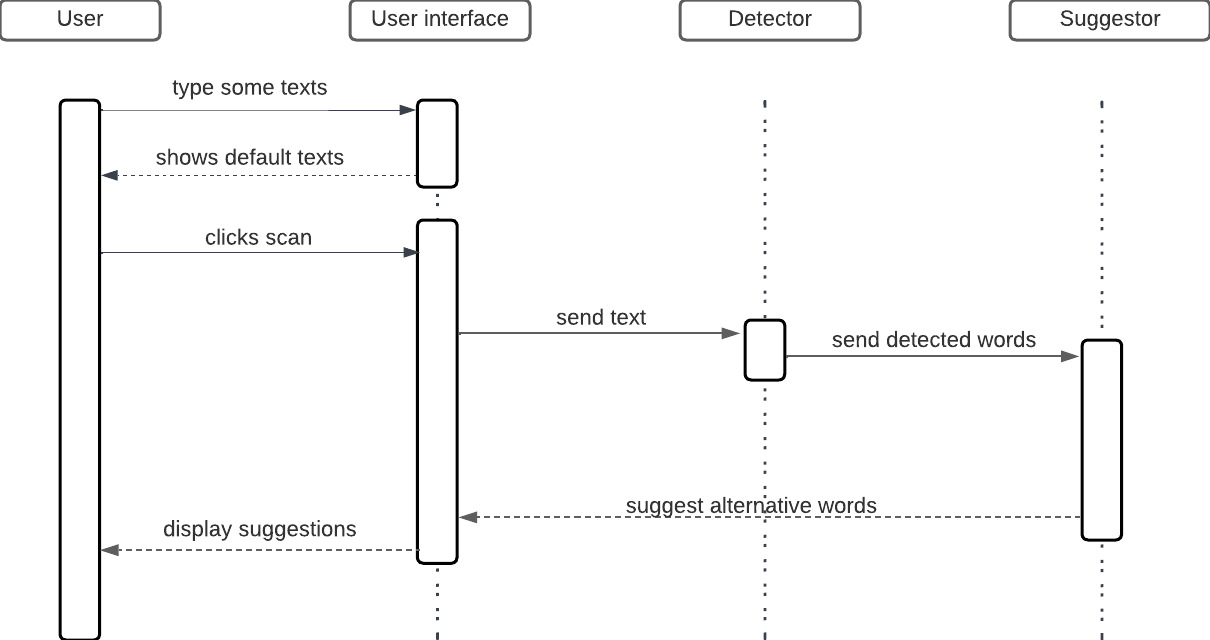
\includegraphics[width=15cm]{./img/chp3/Sequence1.png}
\caption{User text input sequence diagram}\label{fig:seq1}
\end{figure}

Figure \ref{fig:seq1} displays of a normal scenario. when the user inputs texts through the program’s UI. And after they’re done typing and clicking the scan button. Those texts will be sent to the detector's part to detect overused words. Then those overused words will be sent to the suggestor’s part to find alternatives for replacing words and send those word lists back to the UI to display the result to the user.

\noindent{\large\bf  Scenario 2: User accepts the suggestion}
\begin{figure}[!h]\centering
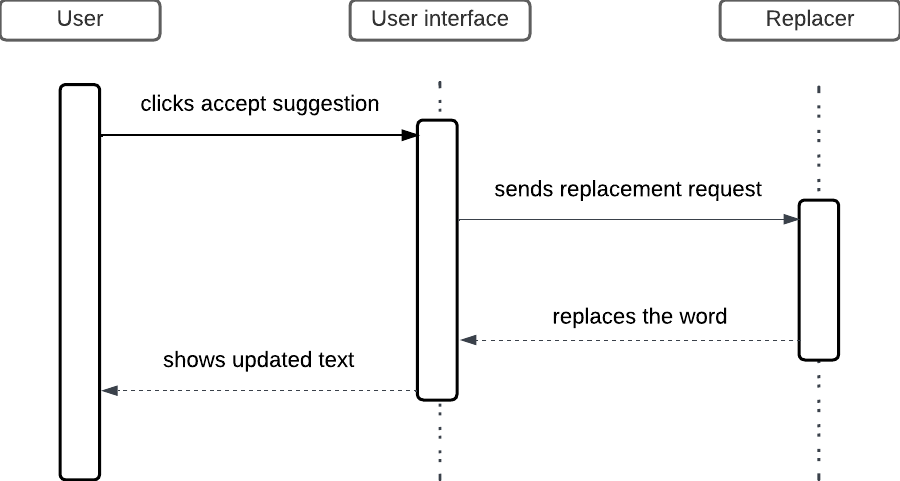
\includegraphics[width=15cm]{./img/chp3/Sequence2.png}
\caption{Rejecting word suggestion sequence diagram}\label{fig:seq2}
\end{figure}

Figure \ref{fig:seq2} shows the process in case the user is satisfied with the suggestion and clicks the accept suggestion button. UI will send this request to the replacer's part, and the replacer will replace the suggestion word into those overused parts throughout the UI. And shows the finalized text.\\

\noindent{\large\bf  Scenario 3: User rejects the suggestion}
\begin{figure}[!h]\centering
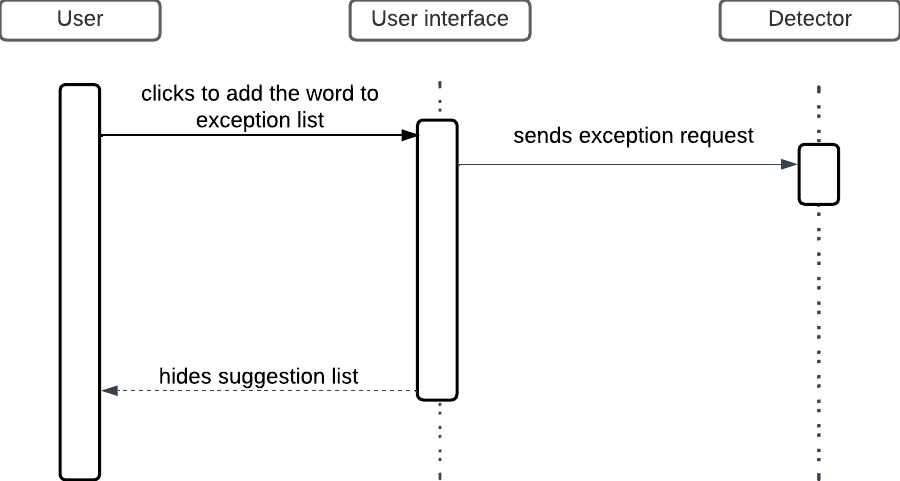
\includegraphics[width=8cm]{./img/chp3/Sequence3.png}
\caption{Accepting word suggestion sequence diagram}\label{fig:seq3}
\end{figure}

Figure \ref{fig:seq3} shows the process in case the user doesn’t want to change this overused word. After they clicked the reject suggestion button. The program will simply hide those suggested word lists for users not to be notified.

\noindent{\large\bf  Scenario 4: User Add the overused word to exception list}
\begin{figure}[!h]\centering
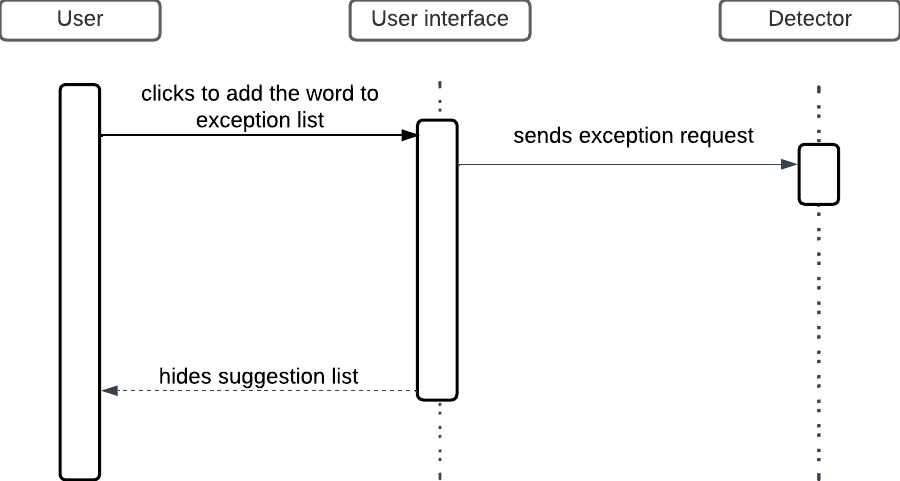
\includegraphics[width=15cm]{./img/chp3/Sequence4.png}
\caption{Adding word to exception list sequence diagram}\label{fig:seq4}
\end{figure}

Figure \ref{fig:seq4} shows the process when the user doesn’t want this overused word to not be scanned at all in the document. So, after they click to add this word to the exception list. The program will send the exception word information to the detector to include it in. And also hide the suggestion list in the UI itself.

\section{User Interface}
\subsection{Input area}
Allow user to input the text either by typing out or copy-and-paste the text.
The words that are marked as overused will be highlighted.
\subsection{Information area}
The side panel will be used to show additional details such as alternative words as well as their definition. 

\begin{figure}[!h]\centering
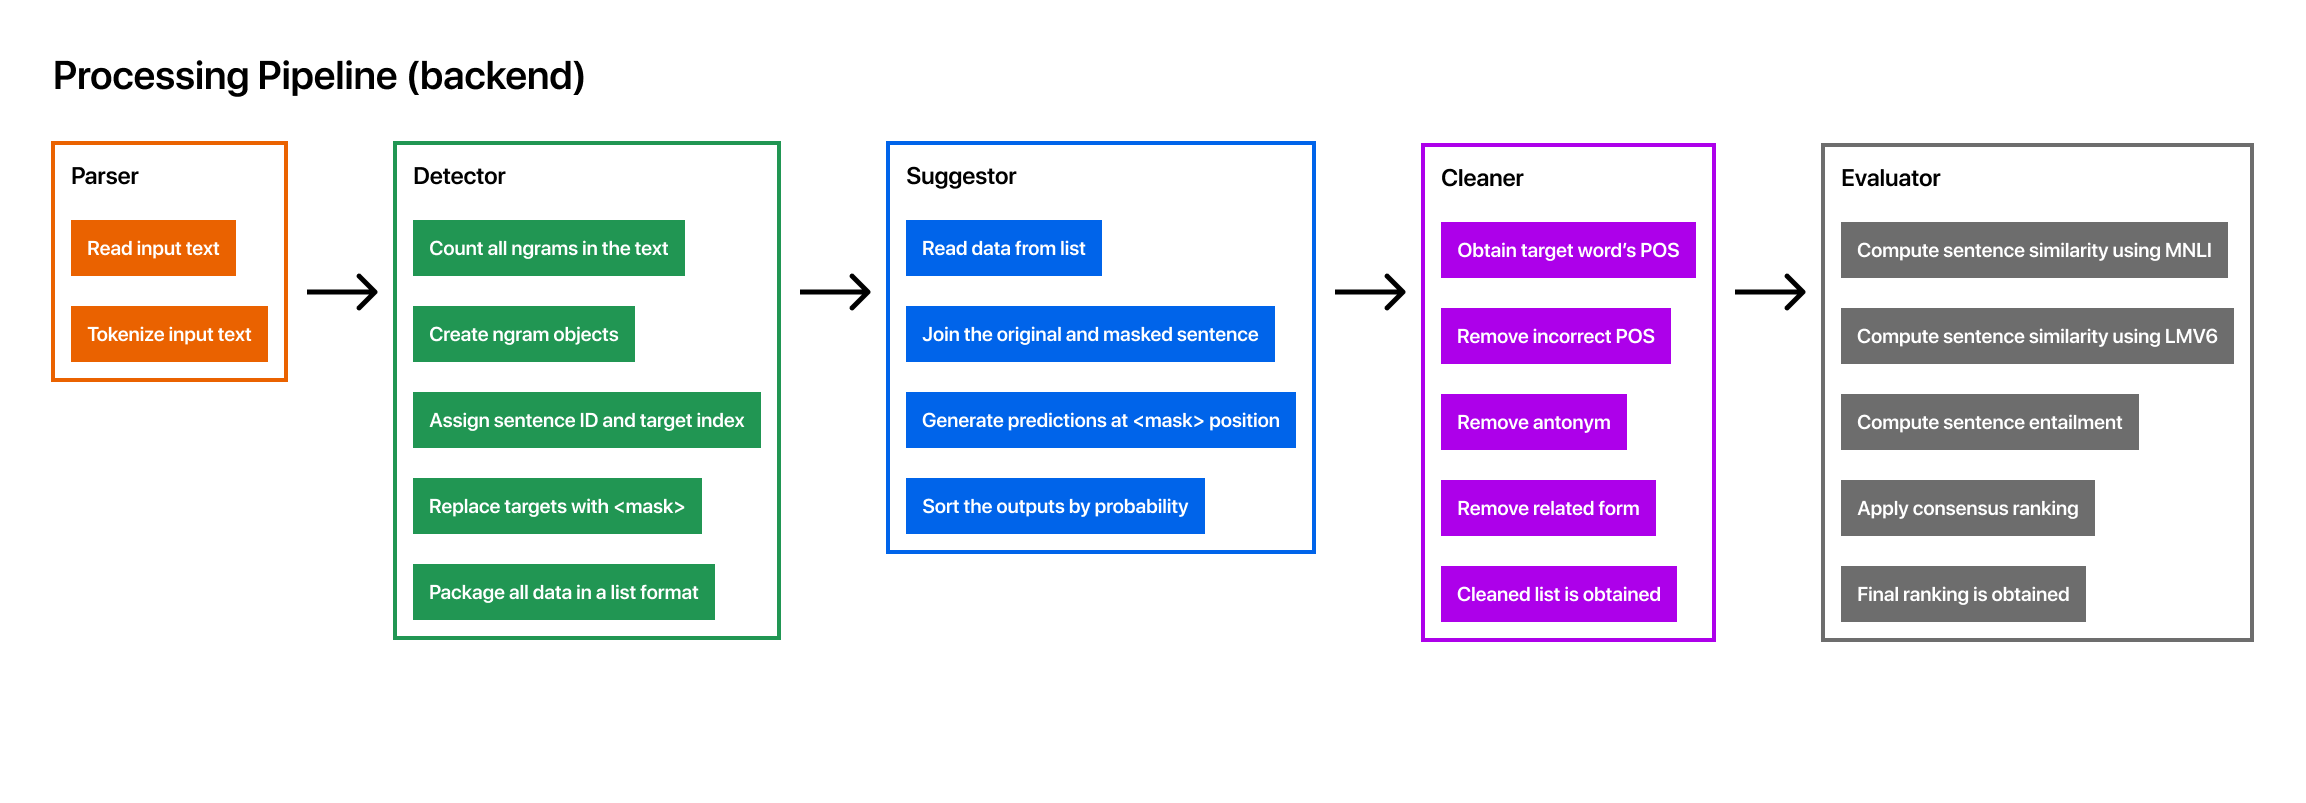
\includegraphics[width=15cm]{./img/chp3/processsingPipe.png}
\caption{Backend logic pipeline}\label{fig:corePP}
\end{figure}
\section{Reader}
\subsection{Read input text}
This program supports both user-typed text and pdf files. In the case of pdf file, the program will extract the text content and tokenize it.
\subsection{Tokenizer input text}
Tokenizer is a task to break input text into individual components known as tokens. This is a critical step and is done before any further analysis can take place. The token can be in a form of a word or sub-word depending on the desired goal. In this project, we need several tokenizers to achieve the goal. For the Parser, we used whitespace tokenizer in conjunction with a Spacy tokenizer. 

\subsubsection{Regex Tokenizer}
Regex Tokenizer proceeds by using regular expressions to match the specified pattern of the input text and then separate them into a token. Currently, the regular expression supports the following cases: Word matching: apple, banana, pencil word with hyphen: plant-based, state-of-the-art, cloud USD currency: 120, 1 abbreviation: U.S.D., N.D. initials containing up to 3 characters: Mr. Mrs. Ph.D. Unlike most out-of-the-box tokenizers which are designed to behave in a specific way, although it is easier to use, altering its behavior is nearly impossible. Some tokenizers such as the one included in Spacy will break apart the contraction (don’t → do n’t) which is not a desirable result for our project. Instead, all contractions must remain as a single token. This is where the regex tokenizer comes in, it is very flexible and can be extended to cover most patterns the way we intended. However, one downside is the performance, some matcher uses greedy search behavior which can increase the execution speed, especially for a long text. After weighing the pros and cons, we decided to go with a regex-based tokenizer due to its flexibility. While working on the project, we noticed that our long and

complex regex tokenizer produced a result comparable to a more simple whitespace tokenizer. Our regex matcher is superior to whitespace only in the case of abbreviations for example Mr. and U.S.A., regex keeps all the dots intact. However, retaining the dot doesn’t add much value to the prediction accuracy of the model. Moreover, our custom regex expression is more prone to errors when dealing with complex text which may contain untested edge cases. Ultimately, we have made the decision to use a modified whitespace tokenizer instead.


\subsubsection{Modified Whitespace Tokenizer}
All the bigram counters will work on the tokens produced by the new modified whitespace tokenizer. Usually, this type of tokenizer splits words by whitespace, however, this means the last word of each sentence will include a full stop. Any word with an extra dot at the end will be counted as a separate item by the n-gram frequency counter. 

I like apple. → apple 
I like apple. → apple.

Thus, the program trims out the excess dots and symbols at the end of each token. This will not affect the accuracy of the prediction.

\subsubsection{Spacy Tokenizer}
The default tokenizer shipped with the package outputs a specific format of tokens that are different from our tokenizer, for example, don’t → do and n’t. All the hyphens are split as a separate tokens. In Spacy, basic tasks such as tokenization, sentence boundary detection, POS, and NER all require a specific model. Our custom tokenization cannot be used in this context. Instead, the default tokenizer shipped with the spacy language package will be used. In Parser, the Spacy tokenizer is used so that we can perform sentence boundary detection, NER, and POS later on in the process


\section{Detector}
The role of this module is to count all the occurrences of n-gram up to trigram in the text. Get the context sentence containing the target word. In the end, it generates a package that will be sent to the sugestor model.
\begin{figure}[!h]\centering
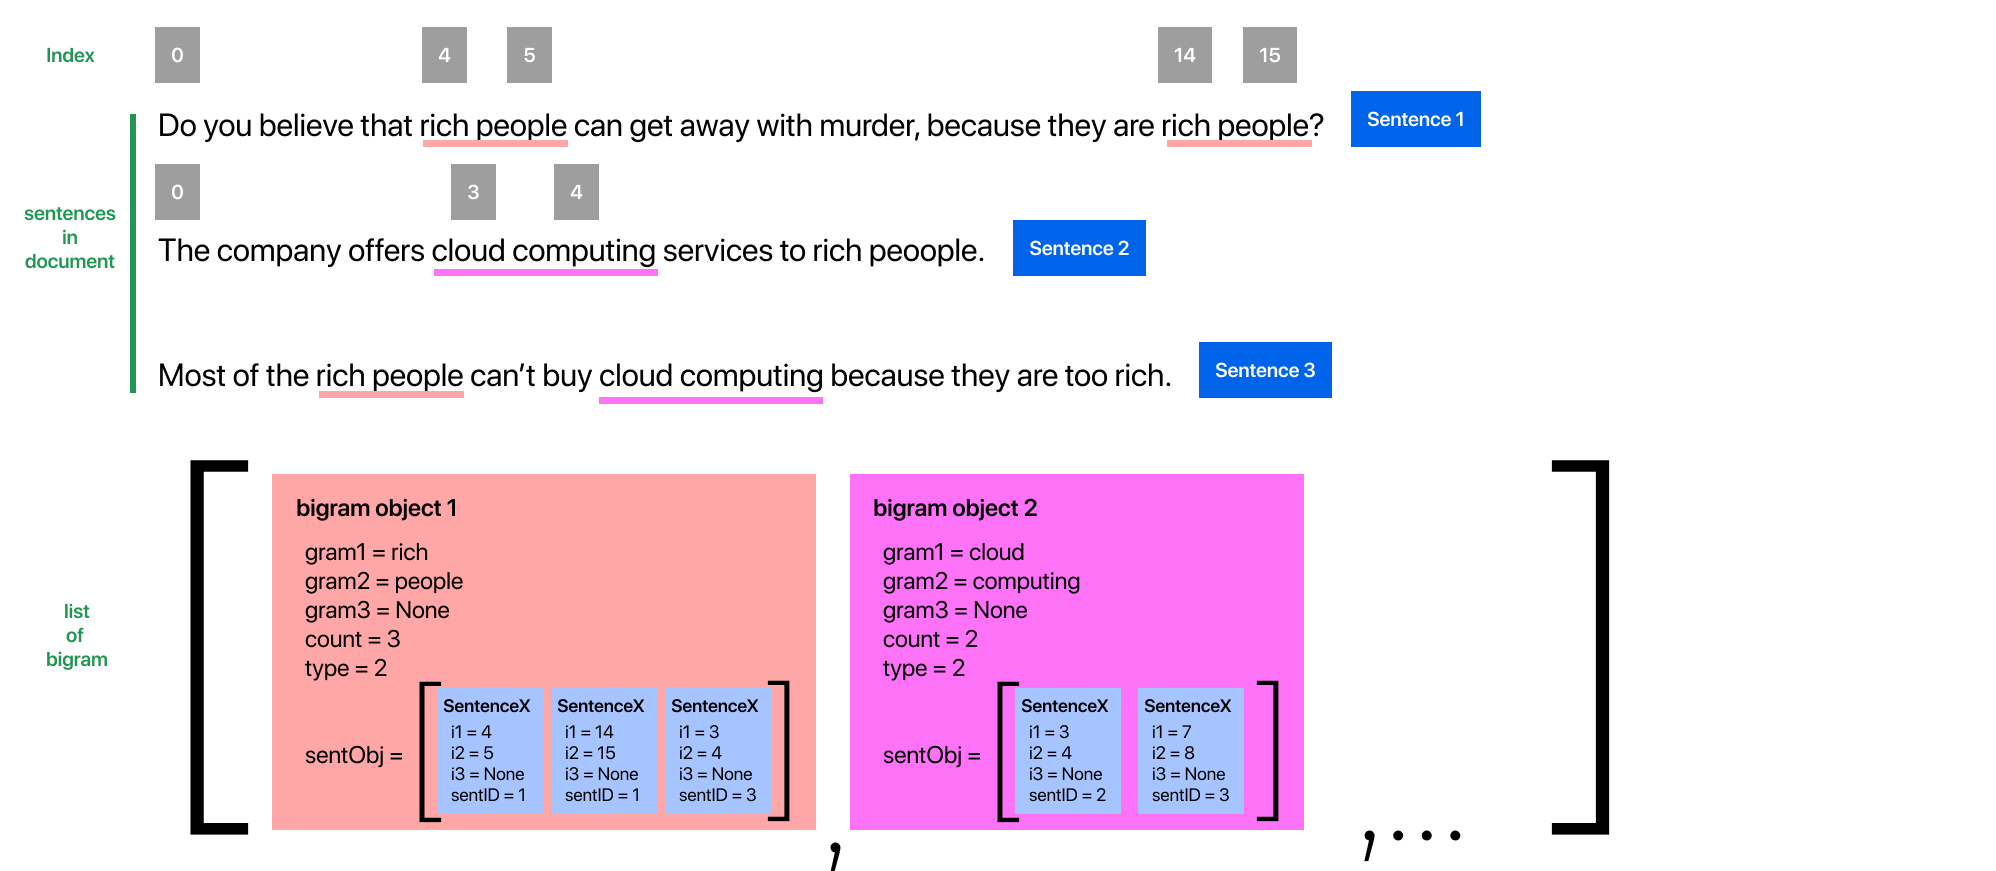
\includegraphics[width=15cm]{./img/chp3/Frame 13.png}
\caption{Structure of n-gram object}\label{fig:list of ngram object}
\end{figure}
\subsection{Count all n-gram in the text}
Detect unigram, bigram, trigram occurrences in the text by counting, the words in the exclusion list will be filtered out to keep only the meaningful words.

\subsection{Create n-gram object}
The detector will generate a list of n-gram objects for each type of n-gram namely unigram, bigram, and trigram. This is a custom object that holds necessary data about he n-gram including individual grams, concatenated ngram, frequency, type, and sentence object list.
\subsection{Assign sentence ID and target index}
  To obtain the context sentence, the program goes through the n-gram list and finds the sentence containing that particular n-gram. All the information is stored in a positional format instead of a full sentence to reduce excessive memory usage. This design decision is made after experiencing multiple out-of-memory crashes caused by other memory-intensive operations of our program. The information is in a cascaded list of objects inside the n-gram object. By doing this, we can directly access the position of the target word during the <mask> replacement process.
\subsection{Repalce target with <mask>}

 Replaces all the target index with <mask> token, if the word is not on the exclusion list. If the word is a part of the list, the replacement will not be performed. 



\subsection{Package all data in a list format}
Finally, the FM (Fill Mask) package containing the original sentence, masked sentence, and the target word is created. This format is sent to the predictor module.

\section{Exclusion List}
In a document, not all words are substitutable, some of them have special grammatical features which if changed, may create ungrammatical sentences. This is particularly true for preposition, modal verb, conjunction, contraction, negation, and pronoun. In NLP, we refer them as a stopword. Thus, the detector will ignore all of the stopwords and will not generate alternatives. Additionally, all the special entities such as name, place, country, work of art, and organization will also be excluded. The following words will be discarded by default: Stopwords such as I, You, We, He, They, Can’t, Could, Will, To, Not, Am, Are Is, Were, Because, etc. Named entity: Location, Name, Country, Work of Art, Person, Organization, etc
If the users do not want to get suggestions for a particular word, they can manually add them to the list as well.




\section{Suggestor}
Roberta, a Robustly Optimized BERT pretraining Approach is used as the main model to generate substitution candidates. The model is similar to BERT but without the next sentence prediction part, leaving with only the masking language modeling (MLM) objective. The primary task is to use MLM to fill in the masked token. For instance, I like playing video game because it is fun. Let’s say we want to replace the word “fun”, we replace it with <mask> token. The sentence “I like playing video game because it is <mask> will be concatenated with the original unmasked sentence to create a sentence pair. The model attempts to predict

the sentence pairs using the context clue from the original sentence with no mask. This approach is used alongside the second approach called embedding dropout which randomly set the target embedding to zero. Without the second approach, the predicted output is very likely to be the original word itself, which is not what we want. We can overcome this issue with the help of embedding dropout.
The candidate generation process begins with the FM package from the Detector module. It contains infor- mation of the following structure The first element, unmasked sentence will be concatenated with the second element, masked sentence, and the third element, target word, will be used to facilitate the evaluation process. 

\begin{figure}[!h]\centering
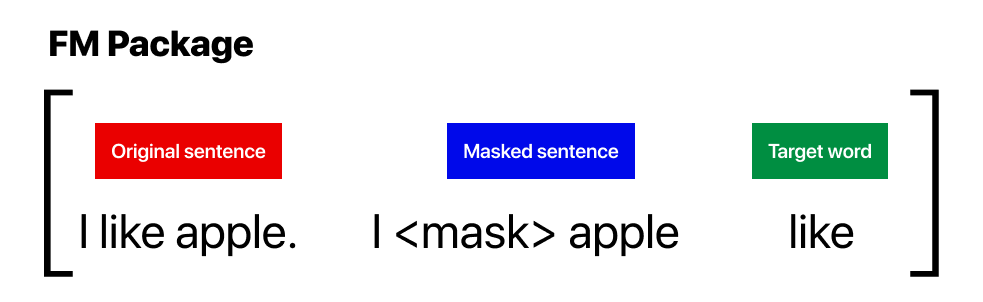
\includegraphics[width=15cm]{./img/chp3/Package.png}
\caption{FM Package (Fill Mask Pacakage)}\label{fig:FMPX}
\end{figure}


\section{Cleaner}
The output candidates still contain a lot of words with incorrect part of speech, verb tense, and non-words. As a result, further cleaning is performed to remove all the wrong items. The following operations will be applied to the candidate list;

\subsection{POS filtering}
Firstly, part of speech of the original word is obtained, next, the part of speech of the all the candidates is obtained. Any word with a mismatched POS with respect to the original word will be removed, leaving only the candidates with the correct POS. Nevertheless, this method is not perfect because sometimes, candidates with wrong verb tense may be tagged incorrectly. Consider this example:


\begin{itemize}
\item[--]I drive Tesla Model X to London. drive is a verb
\item[--]I driver Tesla Model X to London driver is a noun, but it will be tagged as a verb
\end{itemize}
This is due to the tagger being trained to recognize grammatically valid sentences, this sentence is ungram- matical, therefore, unexpected behaviors may occur. 

\subsubsection{Antonym removal}
Secondly, the antonym removal, during this stage, an antonym list is extracted from Wordnet synset database. Words within the antonym list will be removed from the candidate list. 
\subsubsection{Derivationally related form removal}
A derivationally related form is a derived form of the root word. This function removes all variant forms of the word occur in the output list. 

\subsubsection{Inflection removal}
Lastly, inflection removal removes any inflected form of the target word. All of the aforementioned procedures grealtly improve the correctness of the final result. Despite all that, some incorrect word may still be present in the result. 


\section{Evaluator}
Not all generated candidates are a suitable substitution. Although most of them fit in the context well, it changes the meaning of the original sentence entirely. The validation process contains scoring criteria based on semantic similarity between both sentences and lexical relationships extracted from wordnet. A higher score will advance the rank, the lower score will be filtered out if it falls below the threshold.

During the experimentation, we discovered that Wordnet lexical relationships only includes verbs and nouns, but not adjectives. So we cannot rely solely on Wordnet. Our revised strategy employs consensus-based ranking. The technique involves 4 judges, in this project, 4 models are used. The first model is the original ranking based on the raw score of output from the fill-mask pipeline. The second model is called Roberta-base-v2 from Sentence Transformer library. In this project, we use this model to compute sentence similarity against the original sentence. The third model is named Roberta-base-MNLI. It is suitable for computing the similarity between sentences. Lastly, the cross-encoder NLI Roberta-base. This model is used to predict whether 2 sentences entail or contradict each other. NLI is useful for filtering out words that carry the opposite meaning to the original word but are not present in the Wordnet antonym list. This can happen because some words may not explicitly be an antonym according to the dictionary, but in certain contexts, they could be. The words that are marked as contradictory will receive a negative score and pushed toward the bottom. 

\subsection{Consensus Ranking}
All the rankings from each model will be aggregated into the ultimate ranking by considering common posi- tions among all 4 judges. The candidate that is ranked consistently across all 4 rankings will hold its position. In contrast, if there are some disagreements, the final position of a particular word will be readjusted accord- ingly. To elaborate, the word A ranked 3,2,3,4 which is fairly consistent. On the other hand, word B ranked 5,12,9,16, which indicates inconsistency and will need to be reordered using the Borda count algorithm. This method improves average ranking accuracy compared to our previous approach where we relied on a single judge.





%%%%%%%%%%%%%%%%%%%%%%%%%%%%%%%%%%%%%%%%%%%%%%%%%%%%%%%%%%%%%%
%%%%%%%%%%%%%%%%%%%% Experiments %%%%%%%%%%%%%%%%%%%%%%%%%%%%%
%%%%%%%%%%%%%%%%%%%%%%%%%%%%%%%%%%%%%%%%%%%%%%%%%%%%%%%%%%%%%%%
\chapter{Implementation and Result}
This chapter will be discussing the detail and actual implementation, changes, and results of our project.

\section{User Interface}
\subsection{initialize}
\begin{figure}[!h]\centering
\includegraphics[width=15cm]{./img/chp4/Init.png}
\caption{Application’s starting screen}\label{fig:init}
\end{figure}
\begin{figure}[!h]\centering
\includegraphics[width=15cm]{./img/chp4/Bar.png}
\caption{‘File’ button dropdown in the menu bar}\label{fig:bar}
\end{figure}
Figure  \ref{fig:init} shows the program’s blank screen after it’s launched. Showing some basic labels and workspaces including.
\begin{itemize}
\item Menubar: At the top of the window, there’s a bar that contains basic functions such as opening documents, inserting and delete pages.
\item Text workspace: A white blank textbox in the middle of the window, consume most of the window’s area for editing text.
\item Navigation bar: This full width label right below the menu bar includes general functions, easily to see by user. Such as, scan button and page navigation.
\item Sidebar: Showing key functions to look for most repeated words and its suggestion to replace them or
else.
\end{itemize}

\subsection{Opening file}
\begin{figure}[!h]\centering
\includegraphics[width=15cm]{./img/chp4/Open.png}
\caption{Choosing file window}\label{fig:openfile}
\end{figure}
\begin{figure}[!h]\centering
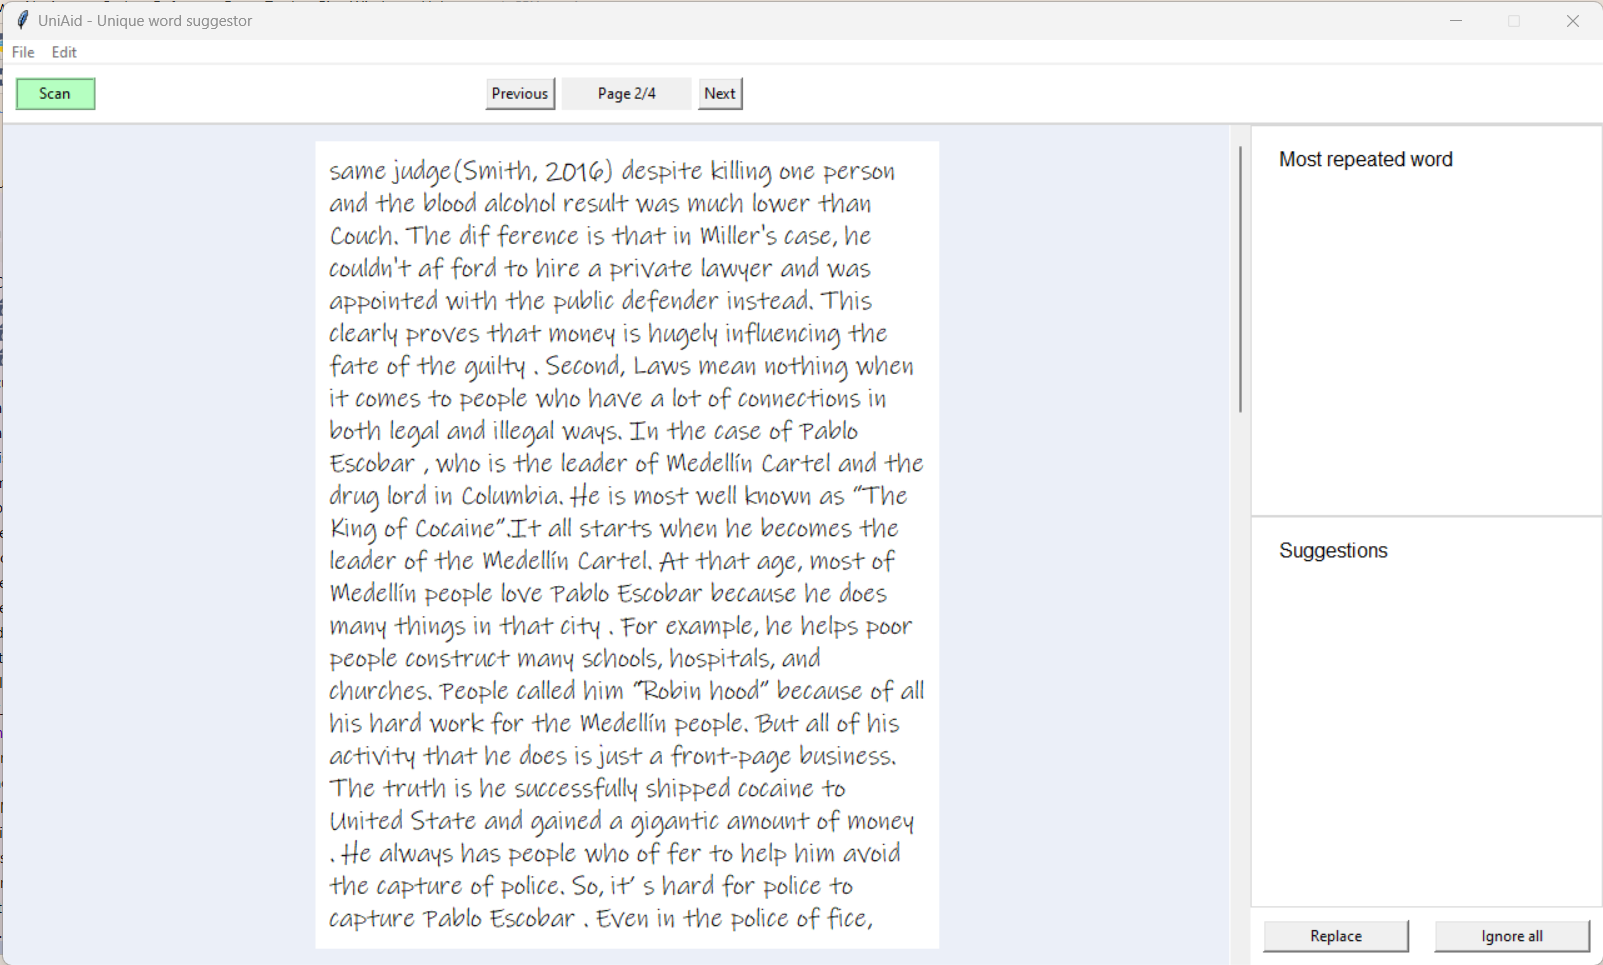
\includegraphics[width=15cm]{./img/chp4/AfterImport.png}
\caption{Application screen after importing the document}\label{fig:afterimport}
\end{figure}
After the user chooses to import the document into the text workspace by going to ‘File’ –> ’Open’ from the menubar shown in figure \ref{fig:openfile}. A File Explorer window will appear to choose .pdf or .txt file. And the application will read the text in the file, then show it in the text workspace page by page, with the page number defined on the navigation bar in figure \ref{fig:afterimport}.

\subsection{Scan function}
\begin{figure}[!h]\centering
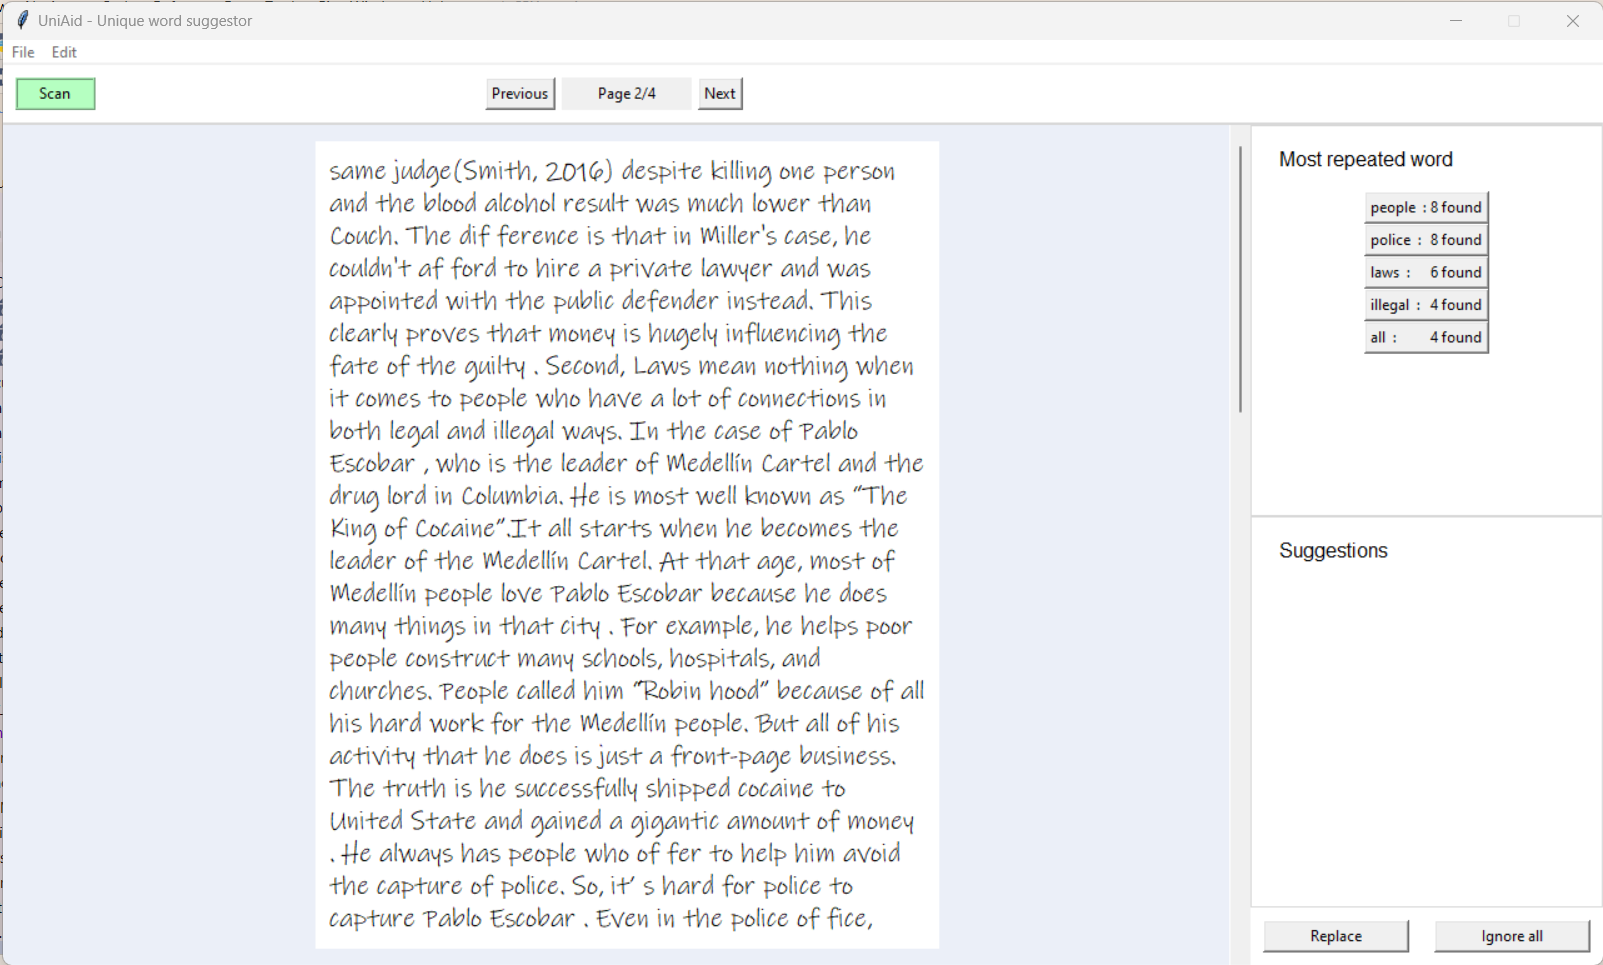
\includegraphics[width=15cm]{./img/chp4/Repeatedword.png}
\caption{Repeated word are showing after scanned}\label{fig:repeatshow}
\end{figure}
After the user has imported the text or scanned the amount of text in the workspace. If they click the green ‘scan’ on the leftmost of navigation bar. The application will scan the text and show most repeated word and each’s current count on the page in the upper side of the sidebar as figure \ref{fig:repeatshow} shows. The repeated word scanned is up to Trigram and without stopwords in any gram.

\subsection{Text highlighting}
\begin{figure}[!h]\centering
\includegraphics[width=15cm]{./img/chp4/Highlight1.png}
\caption{Text of the selected word are highlighted}\label{fig:high1}
\end{figure}
\begin{figure}[!h]\centering
\includegraphics[width=15cm]{./img/chp4/Highlight2.png}
\caption{Different word selecting changes the position of highlight}\label{fig:high2}
\end{figure}
The method of text highlighting has been changed from what it should be in section 3.2.2. As figure \ref{fig:high1} and \ref{fig:high2} shows, after the user clicks on any most repeated word shown in the sidebar. That word in the text will be highlighted light green by using Regex method, captures the exact word as the selected repeated word. Also, The highlight will only show for a single selected word at once.

\subsection{Suggestion}

\begin{figure}[!h]\centering
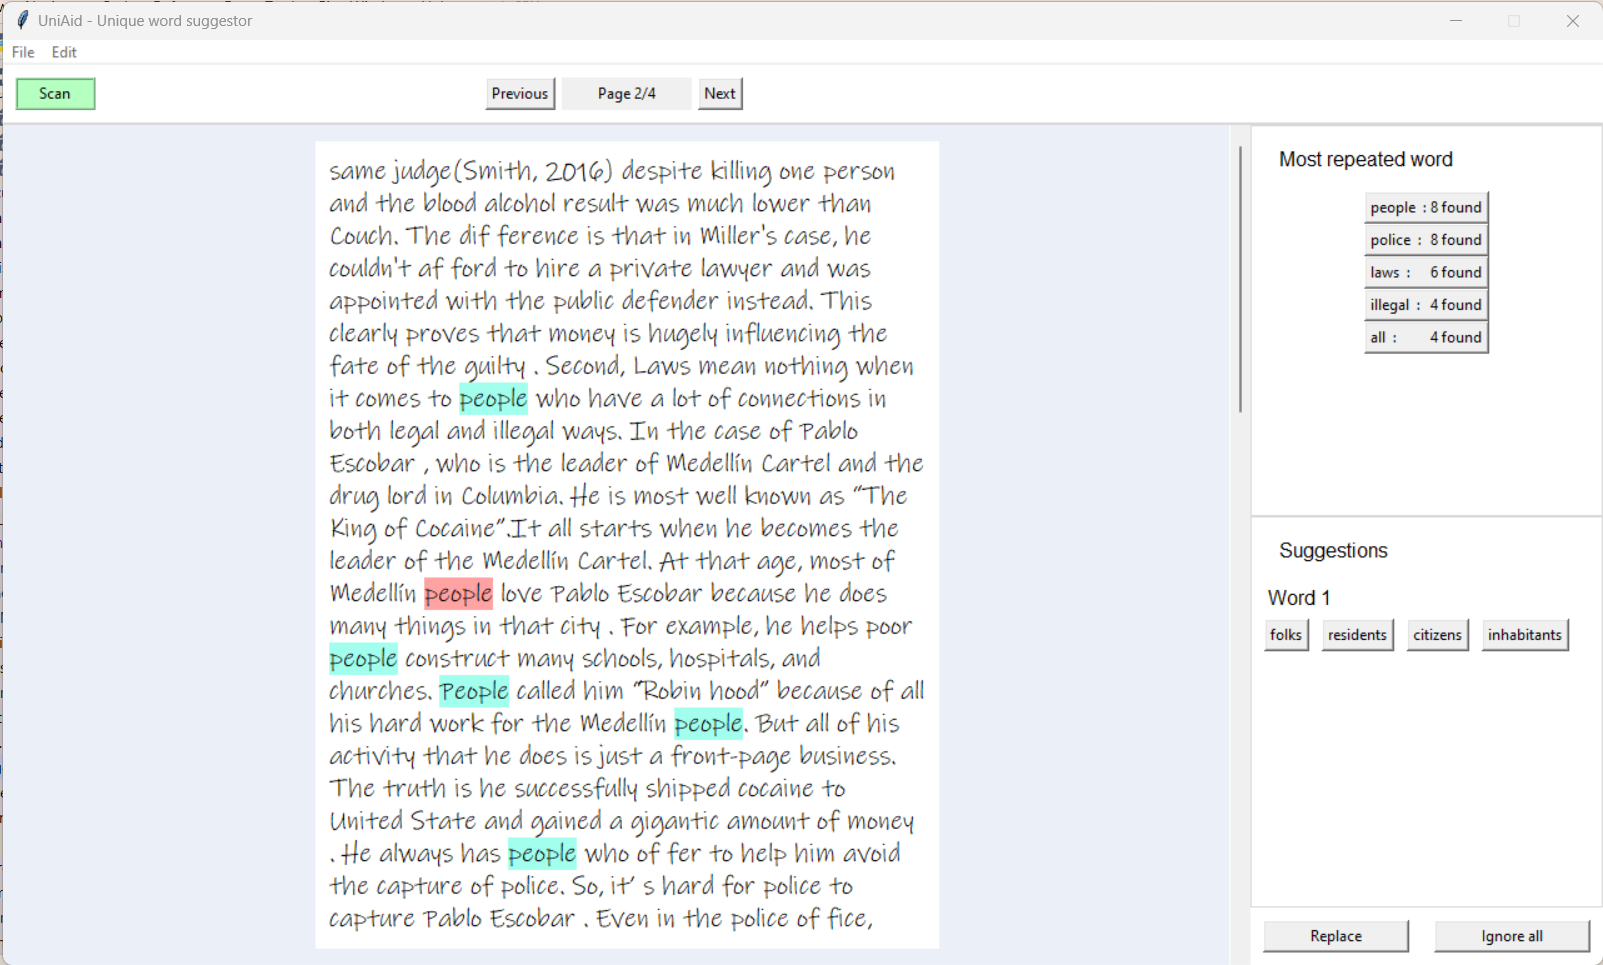
\includegraphics[width=15cm]{./img/chp4/Suggestion1.png}
\caption{Suggestion words shown for the selected word on sentence}\label{fig:suggest1}
\end{figure}
\begin{figure}[!h]\centering
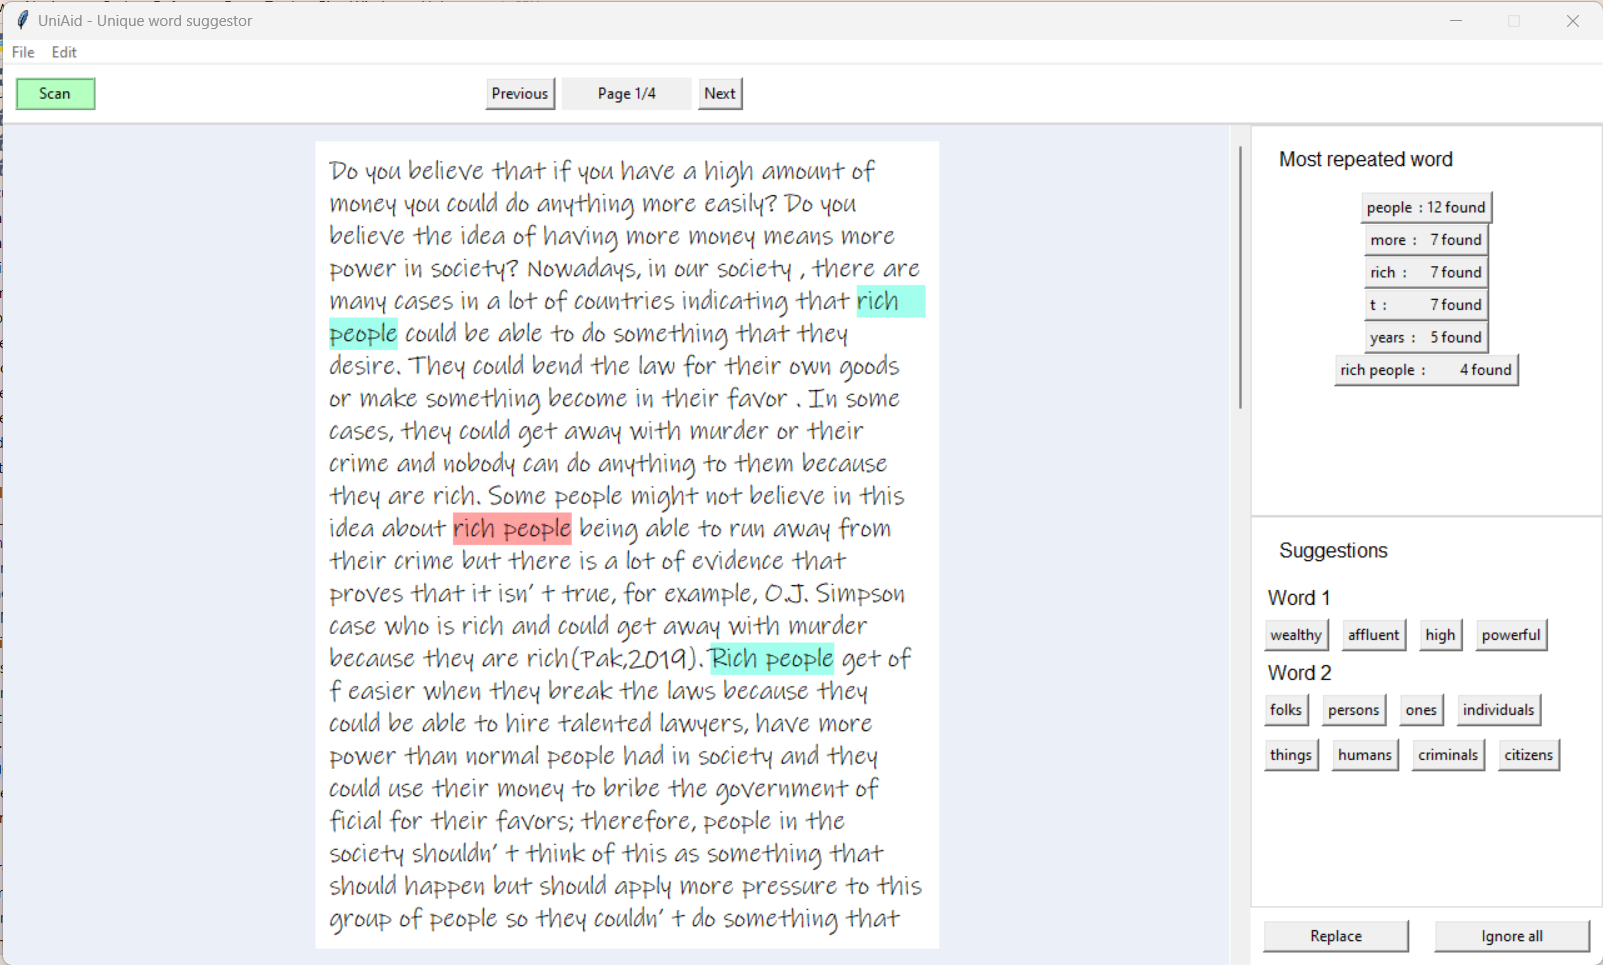
\includegraphics[width=15cm]{./img/chp4/Suggestion2.png}
\caption{Suggestion result of multiple grams word selected}\label{fig:suggest2}
\end{figure}
After the user has selected which word they want a suggestion. And they see that they want a suggestion on a word at a particular sentence. User can click on the highlight on that sentence to make the application starts suggesting. And the selected word are highlighted in red, so the user knows which one they are try to replace. This process takes a moment of time. But after the process is done, on the lower part of sidebar will show list of candidate words as figure \ref{fig:suggest1} shows. Those words has related meaning to the target repeated word, and mostly matches with the context on that sentence which the word is in.

	In case that selected word has multiple grams like in figure \ref{fig:suggest2}. More rows are created at the suggestion tab. Each has a header label which defines its original word that may be replaced. 


\subsection{Replacement}
\begin{figure}[!h]\centering
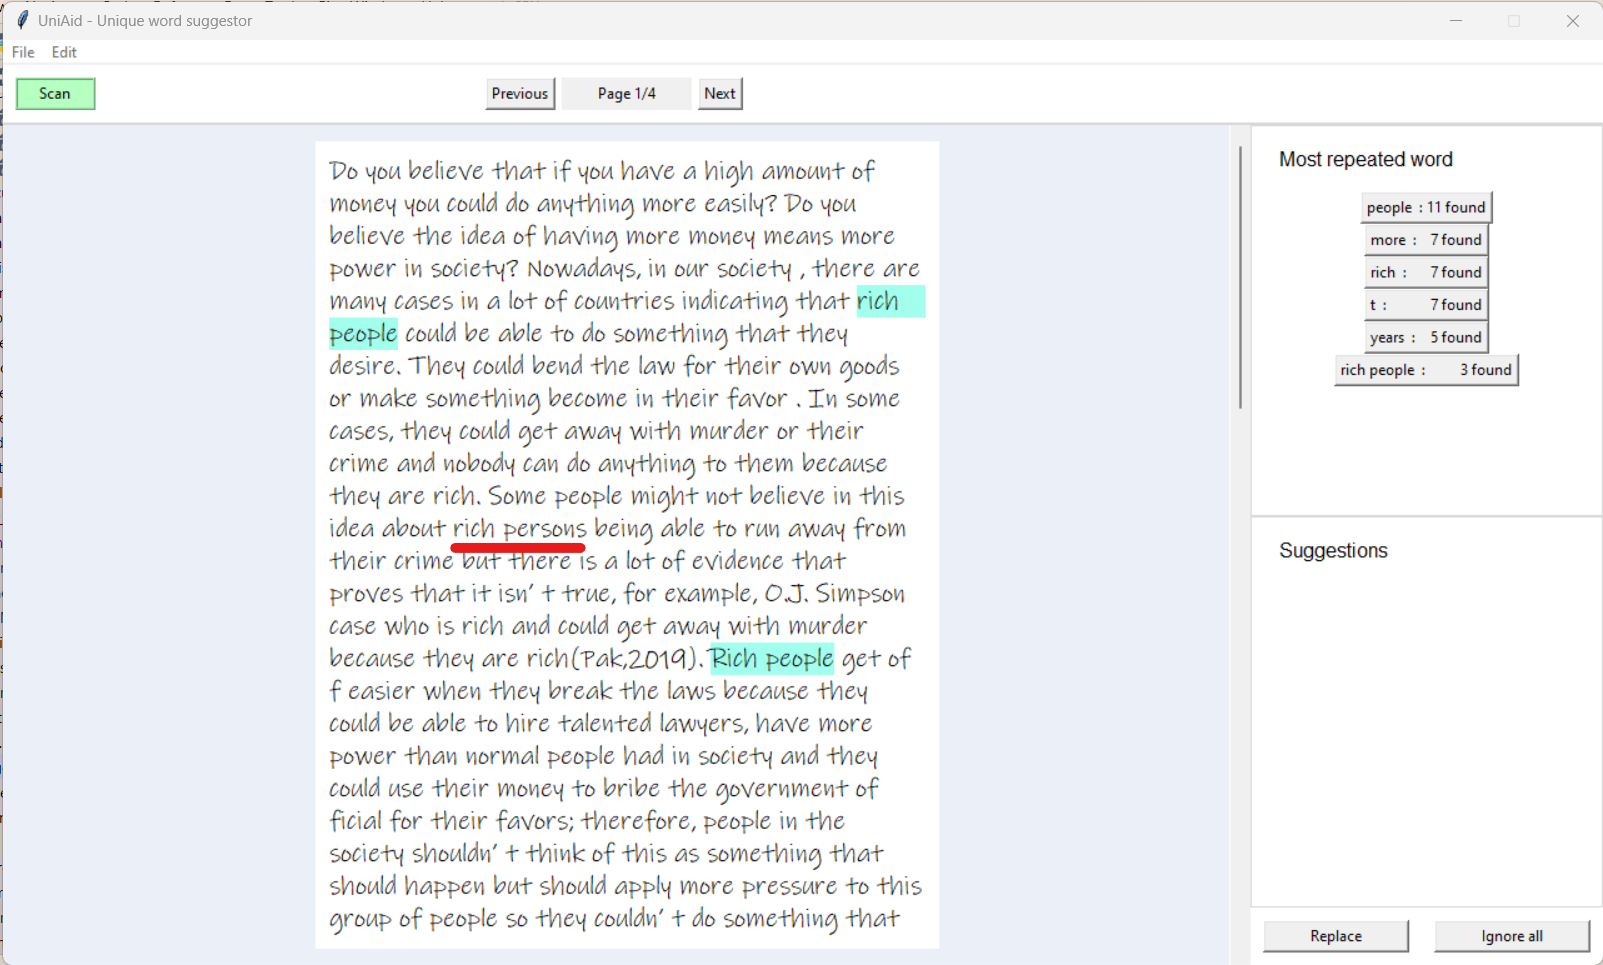
\includegraphics[width=15cm]{./img/chp4/ReplaceMul.png}
\caption{Replacing word on multiple grams}\label{fig:replace}
\end{figure}
If user decided to replace a suggestion word to the repeated word selected. User has to. 1.) Click on the suggested word. 2.) Click on “Replace” button on the leftside of most-bottom of sidebar. And the word is replace, and also rescan the page and highlight the same word selected if it still has too many occurrence. In case that there’re multiple grams. As figure \ref{fig:replace} shows. Users can only select one word to be replaced on the selected gram only.

\subsection{Ignoring words}
\begin{figure}[!h]\centering
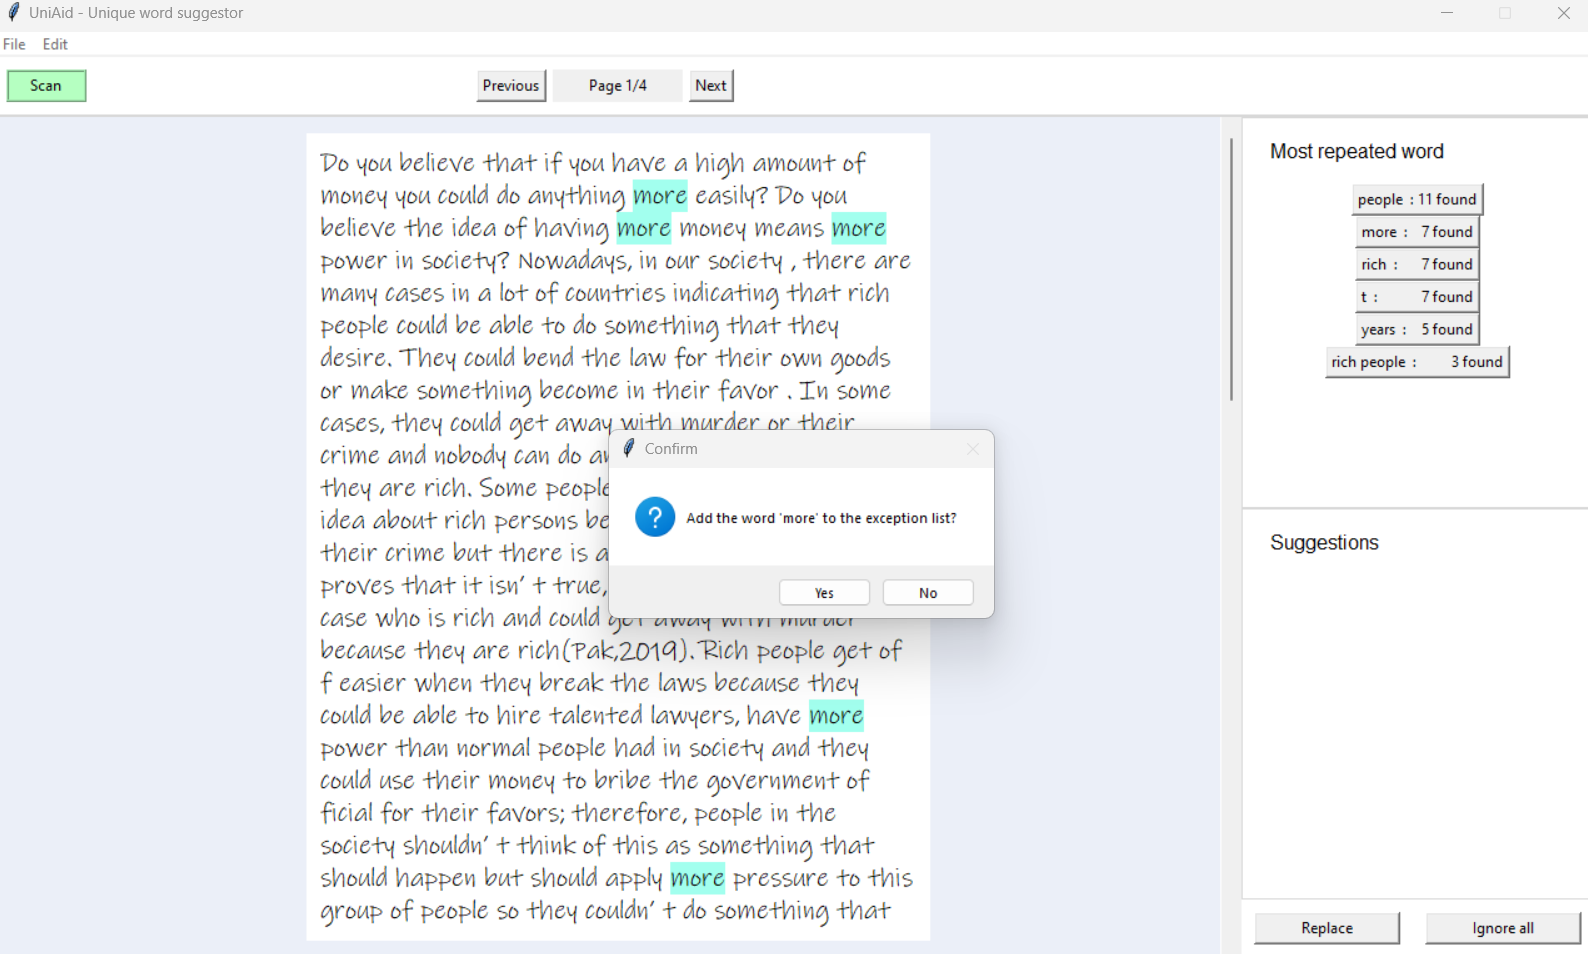
\includegraphics[width=15cm]{./img/chp4/IgnorePrompt.png}
\caption{A prompt to add a word to exclusion list}\label{fig:ignore}
\end{figure}
In case that user don’t want to replace a particular repeated word. The user can click on that repeated word and select ‘Ignore’ button on the lower right corner or the screen. And after user accepts the prompt shown as on figure \ref{fig:ignore}. The application will add that repeated word or grams to the exclusion list which are separately to each other. Which means, adding the word ‘rich people’ to the list, the application won’t ignore the single word ‘people’ or ‘rich’ out of the scanning process and vice versa. 


\section{Application's backend changes}
At the end of midterm, we had a working front-end UI with clickable buttons and a suggesting engine in place. However, both modules were still working on dummy data and did not exchange anything with each other. When combining both sides, we encountered some challenges related to the compatibility between Spacy and Tkinter. As a result, we needed to change a lot of execution orders in the final implementation.
\begin{figure}[!h]\centering
\setlength{\fboxrule}{0.2mm} % can define this in the preamble
\setlength{\fboxsep}{1cm}
\fbox{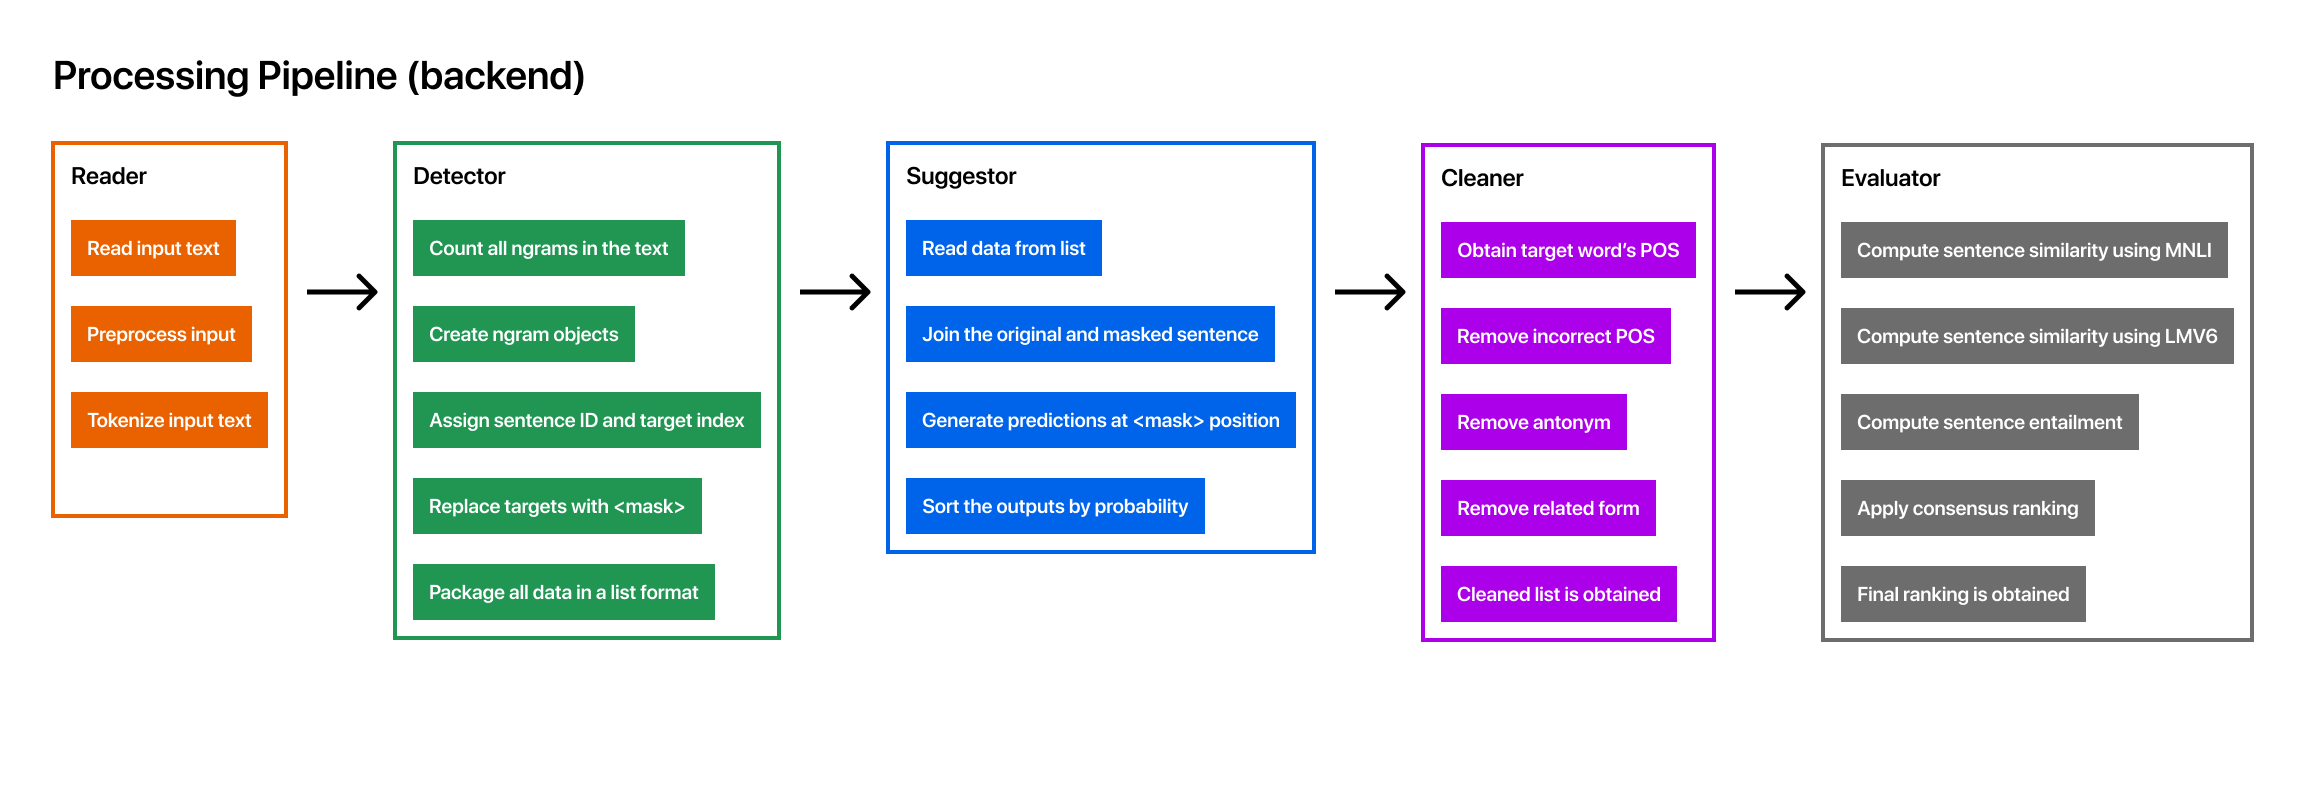
\includegraphics[width=15cm]{./img/chp4/pren.png}}
\caption{Updated pipeline}\label{fig:updated pipeline}
\end{figure}
\subsection{Added Preprocessor}
From the core engine pipeline in chapter 3, we have added a preprocessing step to the Reader component. This stage takes place after the input has been read either from a file or from the input text field. During this process, the following items will be removed from the input text.
\subsubsection{Parentheses}
All the parentheses including square brackets and curly brackets are removed during the input processing which will utilize the Regular Expression to match and replace all the given conditions. The following expression is employed:

\verb/ re.sub("\(.*?\)|\[.*?\]|\{.*?\}|\d+", "", text)/

\subsubsection{Named entity}
Next, the named entity will be marked using Bert-based-NER trained on Named-entity recognition task [Tjong Kim Sang, Erik F.and De Meulder, Fien]. The model will output a dictionary of entities including start, end, string, and entity label. The start and end positions are added to a list called DoNotHighLight. All of the entities will be removed from the text before running the n-gram counter. The cleaning process used Regular Expression to find and replace each entity with an empty string.

The name usually contains 2 tokens which consider a bigram by definition, for example, Steve Jobs, Bill Gates, etc. In the previous version, the program did detect Steve Jobs as a named entity but not until the user clicked the word. This means that anytime the person's name appears in the text repeatedly, it will always show up as a repeated word at the top right panel and the user can click it to get a substitution. However, after the user clicks, the program will perform entity checking right before constructing a Fill-Mask Package, if it is an entity, it will not create any package. Thus, an empty list is passed to the suggestor and an error will be raised. With the new implementation, the highlighter module will check the index against DoNotHighLight list whether or not the word is highlightable.
\subsubsection{Newline character}
In Spacy, all the indexes start from zero at the beginning of the document and continue until the end of the file is reached. On the other hand, Tkinter index in the form of “line.column” runs from the beginning of the line and restarts after a newline character is reached. For example, line 1 char 12 will be 1.12, and line 34 char 0 will be 32.0. Due to this incompatibility, when a newline character is present in the input text, the index will not align with the Spacy index. The correct alignment between both parties is necessary because we need to obtain the parent sentence based on the index of the word user clicked. Therefore, we need to remove any newline character such as \verb/\n \r/ so the index matched up. As a consequence, the input text must not contain any newline otherwise the program will behave incorrectly.
Noting that we did implement the newline handler feature but due to numerous bugs and unexpected behavior it introduced, we decided to discard it entirely.
\subsubsection{Numeric value}
All the numbers are removed from the text before proceeding to the next stage

\subsection{Remove embedding dropout}
After experimenting with Embedding Dropout method, we could not reproduce the result achieved by the original publisher. During the experiment, the produced results were inconsistent and most of them were not usable as a substitution candidate. Thus, we have decided not to use this approach in the final deliverable. The final work only employs sentence concatenation strategy.

\section{Create class objects}
In the revised codebase, some of the backend code has been rewritten to reduce fragmented data and improve readability. With the help of object-oriented, a large number of functions have been grouped under a new class called Parse to simplify the calling process and data passing between the UI and the backend. Note that not all aspects of the project are written using an object-oriented paradigm, most of the code still exists as a function that does not belong to a class. 
\begin{figure}[!h]\centering
\setlength{\fboxrule}{0.2mm} % can define this in the preamble
\setlength{\fboxsep}{1cm}
\fbox{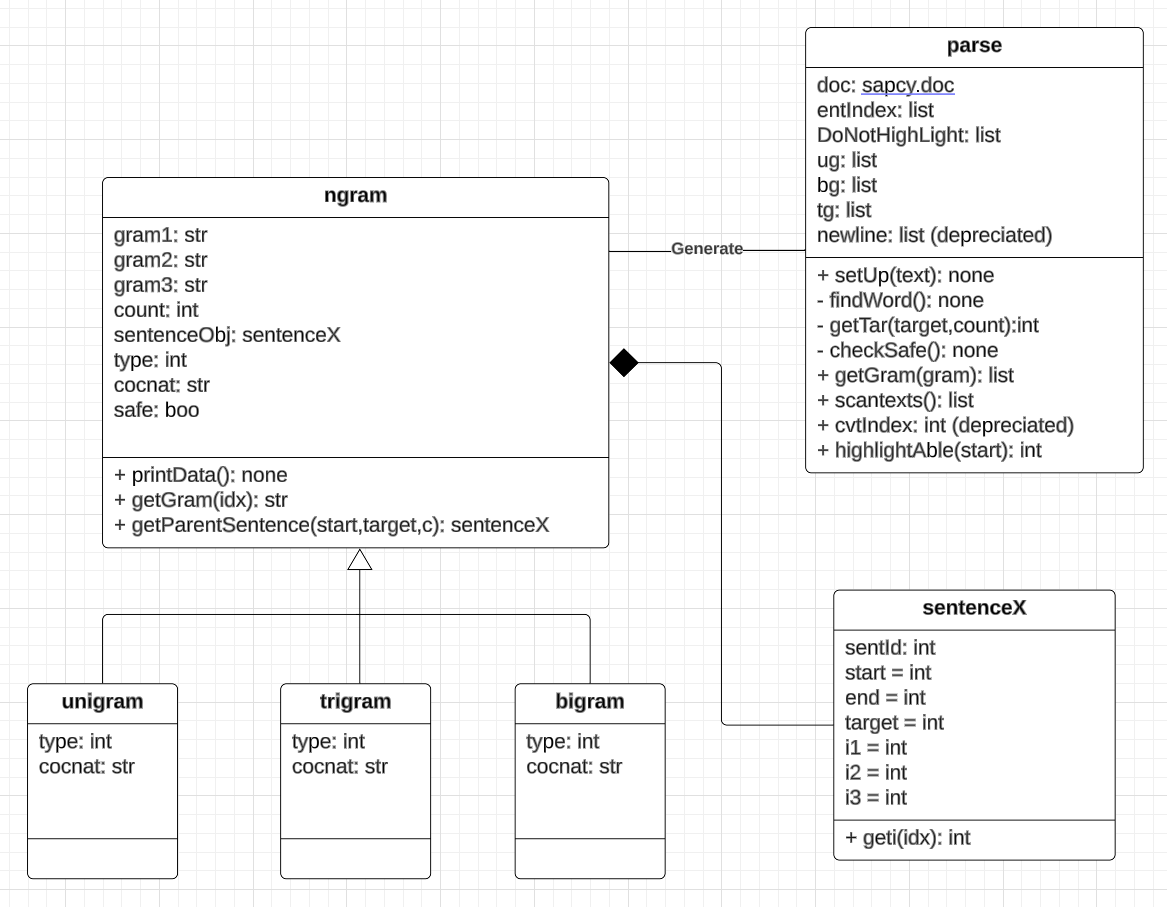
\includegraphics[width=15cm]{./img/chp4/clas.png}}
\caption{Class diagram}\label{fig:class diagram}
\end{figure}
\subsection{ Parse class}
This class contains all the methods for setting up the data. It is responsible for creating and initializing all the necessary data objects as well as providing methods for accessing n-gram and document stored in the class. There are publicly available methods which can be called by another modules and private inner methods which is accessible only within the class.
\subsubsection{Spacy Doc object }
A built-in container class that stores sentence, token, span, span group, and tag data of a particular text. 

\subsubsection{DoNotHighLight list }
Stores the index of named entities detected by the model. This list is constructed by running the named entity recognizer (NER) to obtain all the start positions of the entities. It works in conjunction with the highlightAble() method which will be discussed soon.

\subsubsection{ ug, bg, tg}
Stores a list of unigram, bigram, and trigram objects respectively.

\subsubsection{newline}
Stores a list of newline characters. It is a part of the newline handler feature. (depreciated)

\subsubsection { setUp()} 
Performs various operations sequentially in order to build the objects including sentenceX, n-gram, and Parse object itself. This method is responsible for object initialization, so there is no return value. The execution order inside setUp() method is as follows:

\begin{itemize}
\item clean newline character
\item create spacy doc object
\item create a string version of spacy doc
\item find all named entity
\item append entity index to DoNotHighLight list
\item remove brackets and parentheses using regex
\item remove entity from text using regex
\item tokenize the text string with whitespace tokenizer
\item build n-gram object unigram bigram trigram
\item call findWord() method to fill in data to each n-gram
\item call checkSafe() to flag each bigram 
\end{itemize}

\subsubsection{ findWord()} 
An inner, private method, for obtaining the context sentences that the repeated word is a part of. It will be called by setUp() method. First, it loops through the sentence in the Spacy doc object which stores all the sentence information the document has including start and end index. From there, the modified whitespace tokenizer is used to tokenize the sentence into individual tokens. Next, the code loops through the n-gram object and compare individual gram to each token in the sentence. If the token matched the target gram, it appends that sentence information such as start, end, replacement targets, and sentence id to the sentence object (sentenceX).
\begin{figure}[!h]\centering
\setlength{\fboxrule}{0.2mm} % can define this in the preamble
\setlength{\fboxsep}{1cm}
\fbox{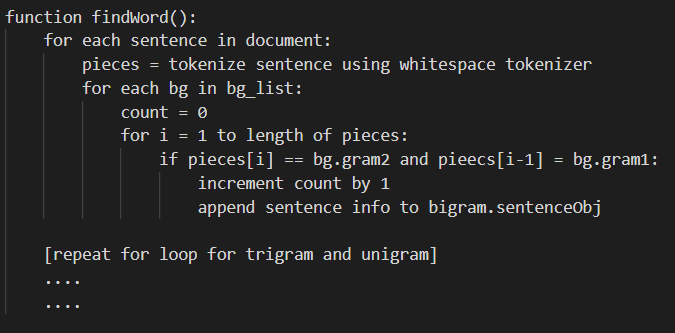
\includegraphics[width=15cm]{./img/chp4/findword.png}}
\caption{findWord() method}\label{fig:findWord() method}
\end{figure}
\subsubsection{getTar() }
An inner, private method that computes the offset of the target word in a given sentence, the output will be stored in the sentenceX target attribute. This method will be called by findWord(), it solves the issue when multiple instances of the same words occur in the same sentence.
\begin{figure}[!h]\centering
\setlength{\fboxrule}{0.2mm} % can define this in the preamble
\setlength{\fboxsep}{1cm}
\fbox{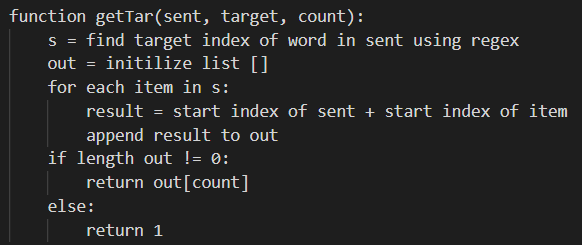
\includegraphics[width=15cm]{./img/chp4/gettar.png}}
\caption{getTar() method}\label{fig:getTar() method}
\end{figure}
\subsubsection{checkSafe}
Checks each gram to make sure it contains no stopword. If any gram of the n-gram is a stopword, the safe flag inside the n-gram object will be set to False, otherwise True. It will be called by setUp().
\begin{figure}[!h]\centering
\setlength{\fboxrule}{0.2mm} % can define this in the preamble
\setlength{\fboxsep}{1cm}
\fbox{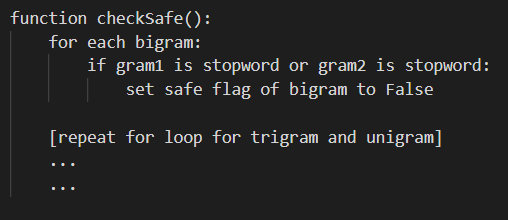
\includegraphics[width=15cm]{./img/chp4/checksafe.png}}
\caption{checkSafe() method}\label{fig:checkSafe() method}
\end{figure}
\subsubsection{getGram()}
Returns a list of the most frequent n-gram including unigram, bigram, and trigram that safe flag is set to True. The list is a mixture of all three grams. It will be called by the UI to display the word in the most repeated word area (upper right corner). 
\subsubsection{cvtIndex()}
A part of the newline handler. (depreciated)

\subsubsection{highlightAble() }
Checks whether the word will get highlighted or not, it will be called before each highlight is applied to the word in the text UI. It works by comparing the index getting from Tkinter to the start and end index in the DoNotHighLight list. It returns 0 for a word that cannot be highlighted, otherwise, returns 1. This is implemented to guard when the repeated word and the entity happened to be the same word, consider the following example, “Star-Lord says the planet called Earth is such a nice place” and “Girls Planet 999 is a Kpop survival show from Mnet. Without this function, both planets will be highlighted while in fact, the highlight should be applied only to the word planet in the first sentence.

\subsection{SentenceX}
The sentenceX object stores all the information about the parent sentence containing n-gram. This object is built through the findWord() method in the Parse class. 

\subsubsection{ start, end }
Hold the start and end indexes of the sentence according to the spacy doc object. The start and end position is obtained through the aforementioned findWord() method. 


\subsubsection{ i1, i2, i3 }
The position of the word to replace with the <mask> token with respect to the output position of the whitespace tokenizer. 

\subsubsection{ target}
In the new implementation, the target attribute has been added. It stores which position of the word to mask in case of multiple instances of the same word present in the same sentence. After combining with the UI, the program will always send the first instance to the suggestor regardless of which word the user clicked. The problem is ultimately solved in the final code by implementing the getTar() method to store its output in sentenceX’s target attribute.

\subsection{Ngram class}
A parent class that is extended to unigram, bigram, and trigram. It stores all information corresponding to its gram.

\subsubsection{gram1, gram2, gram3}
Store each gram separately so it can be individually accessed by another module.

\subsubsection{concat}
Stores concatenated string of all grams. 

\subsubsection{count}
Stores the frequency of the n-gram. 

\subsubsection{ type}
Stores a number corresponding to the n-gram 1 or unigram, 2 for bigram, and 3 for trigram accordingly. 

\subsubsection{ safe }
A flag that will be set to true if all the n-gram contains no stopword, otherwise false. For example, “the planet” → False because it contains “the”. The flag is set via checkSafe() method mentioned previously.

\section{Candidate generation pipeline}

\subsection{Getting raw candidate}
We used the Huggingface Fill-Mask pipeline to predict the most probable candidate at the <mask> position. Before feeding the sentence into the pipeline, we need to apply the sentence concatenation technique. Unmasked sentence and masked sentence are concatenated and separated by space. 

Then, the joined string is passed to the model. The output is in a list of dictionary:



\begin{verbatim}
[{'sequence': "<s>this is sentence one.</s>",
  'score': 0.55454,
  'token': 943,
  'token_str': 'sentence'},...]
\end{verbatim}

The above snippet is a raw output obtained directly from the fill mask pipeline. The information we needed is score and \verb/token_str/, which will be appended to a list, and the rest of the entries will be dropped. After that, we perform candidate pre-cleanup to remove all the duplicated items, then we insert into the target word back to the first position of the list. This allows other modules such as the evaluator and POS filtering to reference the original target word by extracting the first index of the list without the need to pass it as a separate argument. 

\subsection{Candidate clean up}
After getting the raw candidate list the cleaning is performed.
\subsubsection{getMorph()}
First we obtain the POS of every candidates in the list with this function 
\begin{figure}[!h]\centering
\setlength{\fboxrule}{0.2mm} % can define this in the preamble
\setlength{\fboxsep}{1cm}
\fbox{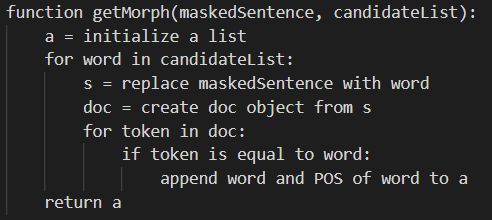
\includegraphics[width=15cm]{./img/chp4/getmorph.png}}
\caption{getMorph() method}\label{fig:getMorph() method}
\end{figure}
\subsubsection{removeMorph()}
Then run the following function to remove all incorrect candidates
The original word is set as a reference, the rest of the candidates will be compared against it.
\begin{figure}[!h]\centering
\setlength{\fboxrule}{0.2mm} % can define this in the preamble
\setlength{\fboxsep}{1cm}
\fbox{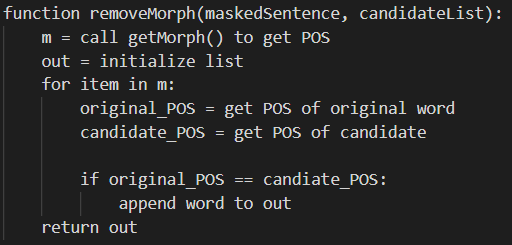
\includegraphics[width=15cm]{./img/chp4/removemor.png}}
\caption{removeMorph() method}\label{fig:removeMorph() method}
\end{figure}
\subsubsection{getAntonym(), getDerived}
It iterates through NLTK WordNet to get the antonym and derivationally related form of the original word. The matches will be appended to a list and a separate function will be executed to remove them from the main candidate list.

\subsubsection{getInflect()}
It lemmatizes the word and tries to get all the inflection possible with a given word. All the inflection will be stored in a list and deleted from the main list.

\subsubsection{additional policy}
Despite the efforts to filter out incorrect items, there are some inappropriate candidates presented in the final list. Those words are not present in any of the aforementioned categories. Take the word ‘manufacture’; the derived form includes ‘manufacturer’, ‘manufacturing’. Unfortunately, both words are not in any of the related forms or inflected words. Therefore, we have to use the Levenshtein ratio to compute the similarity of the words based on how close they are literally. The candidates will be compared from top to bottom. The downside is that we may miss some candidates that are suitable for the context.

\subsection{Candidate evaluation}

The candidates are evaluated using ranking obtained from different models namely, 
\begin{verbatim}
sentence-transformers/stsb-roberta-base-v2 
textattack/roberta-base-MNLI
cross-encoder/nli-roberta-base
roberta-base (raw score obtained from fill-mask probability output)

\end{verbatim}



\subsubsection{Sentence similarity }
The task this function performs is to calculate sentence similarity score using cosine similarity. Only the first 2 models will be passed to the sentenceSimilarity(), one at a time. The new sentence is generated by replacing the <mask> with candidates, it will be compared against the original sentence. The output will be sorted by score in descending order.
\begin{figure}[!h]\centering
\setlength{\fboxrule}{0.2mm} % can define this in the preamble
\setlength{\fboxsep}{1cm}
\fbox{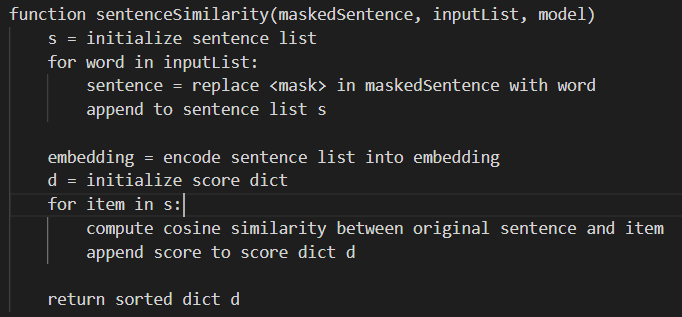
\includegraphics[width=15cm]{./img/chp4/sentencesim.png}}
\caption{sentenceSimilarity() function}\label{fig:sentenceSimilarity() function}
\end{figure}


\subsubsection{Sentence entailment}
The third model will be used to perform token classification in entailment(), the purpose of it is to categorize 2 sentences into entail, contradict, or neutral. 
This function first obtain the base score from sentenceSimilarity() the output score will be summed with the entailment score and the newly calculated score will be sorted and return. The intention of this is to suppress the antonym and low-quality candidates by giving them a negative score, so those words will be ranked lower in the final aggregated list.
\begin{figure}[!h]\centering
\setlength{\fboxrule}{0.2mm} % can define this in the preamble
\setlength{\fboxsep}{1cm}
\fbox{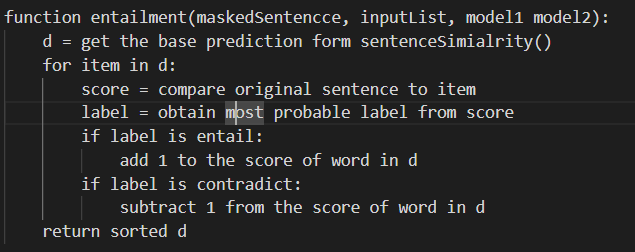
\includegraphics[width=15cm]{./img/chp4/ential.png}}
\caption{entailment() function}\label{fig:entailment() function}
\end{figure}






\subsubsection{ Consensus ranking:}

The consensus ranking involves calculating the average position across all the judges. It first aggregates the positions from all 4 judges into a dictionary representing the rank given by each judge. 
\begin{verbatim}
Rank from judges
judge1: [[word1,rank1],[word2,rank2],[word3,rank3],...]
…
…
judge4: [[word1,rank1],[word2,rank2],[word3,rank3],...]

\end{verbatim}
Aggregated dictionary: 
\begin{verbatim}
{word1:[judge1_rank, judge2_rank, judge3_rank, judge4_rank],...}
\end{verbatim}
The final ranking is obtained by calculating the average rank among all 4 judges.


\section{Performace improvement}
\subsection{Refactoring model initialization }
According to the term 1 presentation, we were concerned about the time taken to perform the computation. Back then we assumed the problem was related to the complexity of the model so we switched from Bert to Roberta. Since Roberta removed the next sentence prediction as stated in Chapter 2, the computation complexity should decrease theoretically. Nonetheless, after investigating, we found out that the major bottleneck did not cause by the model complexity but by our poor coding structure. In the old version, we reload the model every time we wanted to predict and verify the candidate. The total raw output is about 30 to 40 candidates per prediction. A single model took 12 seconds on average to load, we have 3 of them in total. To demonstrate, try multiplying 40 by 12, the program will take at least 480 seconds for one model to reload excluding the time where the actual calculations take place. By refactoring the code, we can get the model loading part out of the loop and load all the models only at the beginning of the program. This dramatically reduced the wait time to the acceptable threshold. Moreover, the change has been extended to other modules involving model loading, for example, Spacy.load(en core web lg) model in the Parse class.

\subsection{Threading}
In the previous version, the UI and the core engine were executed on the same thread. Leads to the program appear not responding after the button is clicked and the backed logic is running. At this stage, the program became frozen, while in reality, it is only the UI that is hanging. The overall program is still working fine, and the "this program is not responding" message will resolve once the background computation is completed. Undoubtedly, this leaves the users with a bad user experience and we need to address this issue. The solution is to figure out a way to run the front-end UI and the backend logic on a separate thread so both processes can run concurrently. We use threading library built into Python to create 2 threads one for UI one for the backend. In the current version, the problem has been solved successfully.



\subsection{GPU acceleration}

Our project utilized PyTorch library which supports GPU acceleration through the CUDA (Compute unified device architecture) Compute toolkit from Nvidia. It is a library that allows the developer to use GPU for general-purpose computing. In theory, the approach used in this project will benefit from parallel computing power of the GPU, it should speed up the calculation significantly. However, our GTX 1050 only has 4gb of VRAM which is not enough to hold the data for the model. Therefore, we need to go back to using the CPU instead.
\section{Model finetuning}

For the data modeling side. We have tried Model finetuning on a custom dataset, but it doesn’t work as in- tended. As a part of our initial plan, we need to retrain the model on a custom dataset focusing on the academic document. The dataset we collected is from the open-source arXiv research paper abstract containing 1.7 million articles with a size of 3GB. Due to a large amount of data and task complexity, the finetuning process was executed on Google Colab Pro+ with the help of GPU acceleration. We finetuned Roberta-large and Roberta-base which used Masked Language Modelling during the training process. This technique required only the actual text data, so all the unnecessary columns including metadata, labels, and URL to full text were discarded. 

The code we used to finetune the model is adapted from the “Fine-Tuning for Domain Adaptation in NLP” by Marcello Politi \cite{s}
The original poster utilized the Huggingface’s DataCollatorForLanguageModelling to prepare the data for that is suitable for masked language modeling task. We modified the data processing step to take our data from arXiv as input \cite{t}. 
 
During our first attempt, we used an entire 1.7 million sample to train, unfortunately, it quickly consumed a huge amount of compute units and took almost 6 hours to complete. Despite a Pro+ subscription, there was not much room for experimentation due to the resource limit. As a consequence, we needed to shrink the size from 1.7 million to 440K, which reduced resource utilization but accuracy will surely affect the accuracy. We were able to achieve 5 attempts. We tried adjusting the parameters namely learning rate, batch size, decay, and the number of epochs. The lowest loss we achieve was 1.29 after 8 epochs. Regardless, the performance of the finetuned model was not satisfactory. It performed no better than the original out-of-the-box model for both Roberta-base and Roberta-large.


\section{Testing strategies}
After we have all required functions in our application. We also have to test the system if there’s any case that makes the application can’t run further and solve those problems.

The scope of testing is the actual application including all supporting module that combines with the main file which runs the UI and makes the application run as intended. And the test doesn’t include the model training files which we use before creating the application but doesn’t use in it.

We will do the functional test on each unit, test each possible input or an empty input and verify that it’s running as expected. Such as the process of opening the file, if we cancel halfway or input other types of files, we will check the result and fix if there’s an error occurred. The same goes for component test and system tests. And also comes up with one major logic to handle inappropriate action between modules.

\section{Data resetting logic}
In order to avoid unnecessary error or mistake occurred by some user action across modules such as select replacing words then change page and replaces after that, which interacts to values in multiple files not properly in order and should make the application not functioning normally. So there should be a functions insertion based on the logic to reset data and values sorted as priority according to the interaction process below. 
\begin{verbatim}
	Textbox →  Repeated word → Highlighted word→ Suggestion word
\end{verbatim}
Which means resetting at the ‘Textbox’ level will clear texts in every page, repeated word list, any highlights showing and the suggestion word list. So we have cover the function in these action according to the priority level.

\begin{itemize}
\item ‘New’ option in the menu bar will clear values at the ‘Textbox’ level and the following data.
\item ‘Open’ option in the menu bar will replace the textbox with the new text and clears value at the ‘Textbox’ level and the following data.
\item Scanning, replacing suggestion word, ignoring repeated words, and changing pages will clear values at ‘Repeated word’ level and the following data.
\item Clicking another repeated word will clear values at ‘Highlighted word’ level and the following data.
\item Clicking another highlighted word will clear values at ‘Suggestion word’ level.
\item Clicking another suggestion word won’t clear any values.
\end{itemize}

\section {Evaluating suggestion}

\textbf{Intrinsic evaluation}\\
Intrinsic evaluation involves assigning human annotators to directly verify the quality of substitutions.
Each of them will determine the correctness and appropriateness of the candidates in a given context which can be in the form of binary or scale rating. In binary, the judge can only assign a word as appropriate or inappropriate as opposed to in scale rating, where the judge will rate the level of fitness based on a scale given by the instructor.
The binary scheme focuses on overall acceptability of the generated candidates rather than capturing the fine-grained nuances as in scale rating. Intrinsic evaluation can also be performed against ground truth data usually obtained through crowdsourcing or text pre-annotated by humans.
\\\\
\textbf{Extrinsic evaluation}\\
Instead of directly measuring the quality of generated output directly, this approach aims at evaluating the system based on the impact it has on the performance of other NLP tasks. We might ask, does the generated candidate improve the generalization of a particular token classification model? Or does it improve the question-answering model? If the performance improvement in downstream is substantial, it implies that the quality of the output substitutions is proven to be useful\cite{r}. 

In this project, intrinsic evaluation is used to assess the quality of generated words.

\subsection{Final VS Raw output}
The table below illustrates the top 15 rankings from the final output which has been reranked using consensus ranking and raw output which is the raw ranking from the model without any operation applied including all the cleaning procedure and consensus ranking.
\\
According to the table, some candidates with wrong part of speech are still present in the list this is due to the POS tagger misclassified the word. The issue arises because the tagger can only handle grammatically correct sentences, however, the predicted output from the model is not always in the right part of speech. As a consequence, when substituting those words in the <mask> position, the tagger will give an incorrect result. 
\\\\




\begin{tabular}{ll}
\hline
\textbf{Final output (rerank)} &
\textbf{Raw output} \\ \hline

\begin{tabular}[c]{@{}l@{}}{[}'highlighted', 'stressed', 'emphasized', \\ 'outlined', 'reiterated', 'noted', 'elaborated', \\ 'promoted', 'explained', 'centered', 'expressed',\\  'addressed', 'illustrated', 'advocated', 'demonstrated'{]}\end{tabular} &
  \begin{tabular}[c]{@{}l@{}}{[}'emphasized', 'stressed', 'emphasizes', \\ 'emphasizing', 'highlighted', 'explained', \\'reiterated', 'emphasize', 'outlined',\\ 'promoted', 'appreciated', 'elaborated', \\ 'exaggerated', 'addressed', 'increased'{]}\end{tabular} \\ \hline
\begin{tabular}[c]{@{}l@{}}{[}'strongly', 'strong', 'substantial', 'robust', \\'significant',  'vigorous', 'high', 'sharp',\\ 'prominent', 'powerful', 'close', \\ 'highly', 'good', 'firm', 'solid'{]}\end{tabular} &
  \begin{tabular}[c]{@{}l@{}}{[}'strong', 'stronger', 'strongly', 'weak', \\'strongest', 'robust', 'powerful', \\'substantial', 'strength', 'strengthened', \\ 'high', 'large', 'vigorous', 'close', 'strengthening'{]}\end{tabular} \\ \hline

\begin{tabular}[c]{@{}l@{}}{[}'manages', 'handles', 'processes', 'addresses', \\ 'tackles', 'controls', 'treats', 'covers',\\ 'oversees',  'uses', 'supports', 'carries',\\ 'deals', 'governs', 'contains'{]}\end{tabular} &
  \begin{tabular}[c]{@{}l@{}}{[}'handles', 'processes', 'manages', 'treats',\\ 'handle',  'deals', 'performs', 'handling',\\ 'considers', 'conducts', 'handled',\\ 'approaches', 'uses', 'supports', 'addresses'{]}\end{tabular} \\ \hline
\end{tabular}



\subsection{The effect of consensus ranking}
\begin{figure}[h]\centering
\setlength{\fboxrule}{0.2mm} % can define this in the preamble
\setlength{\fboxsep}{1cm}
\fbox{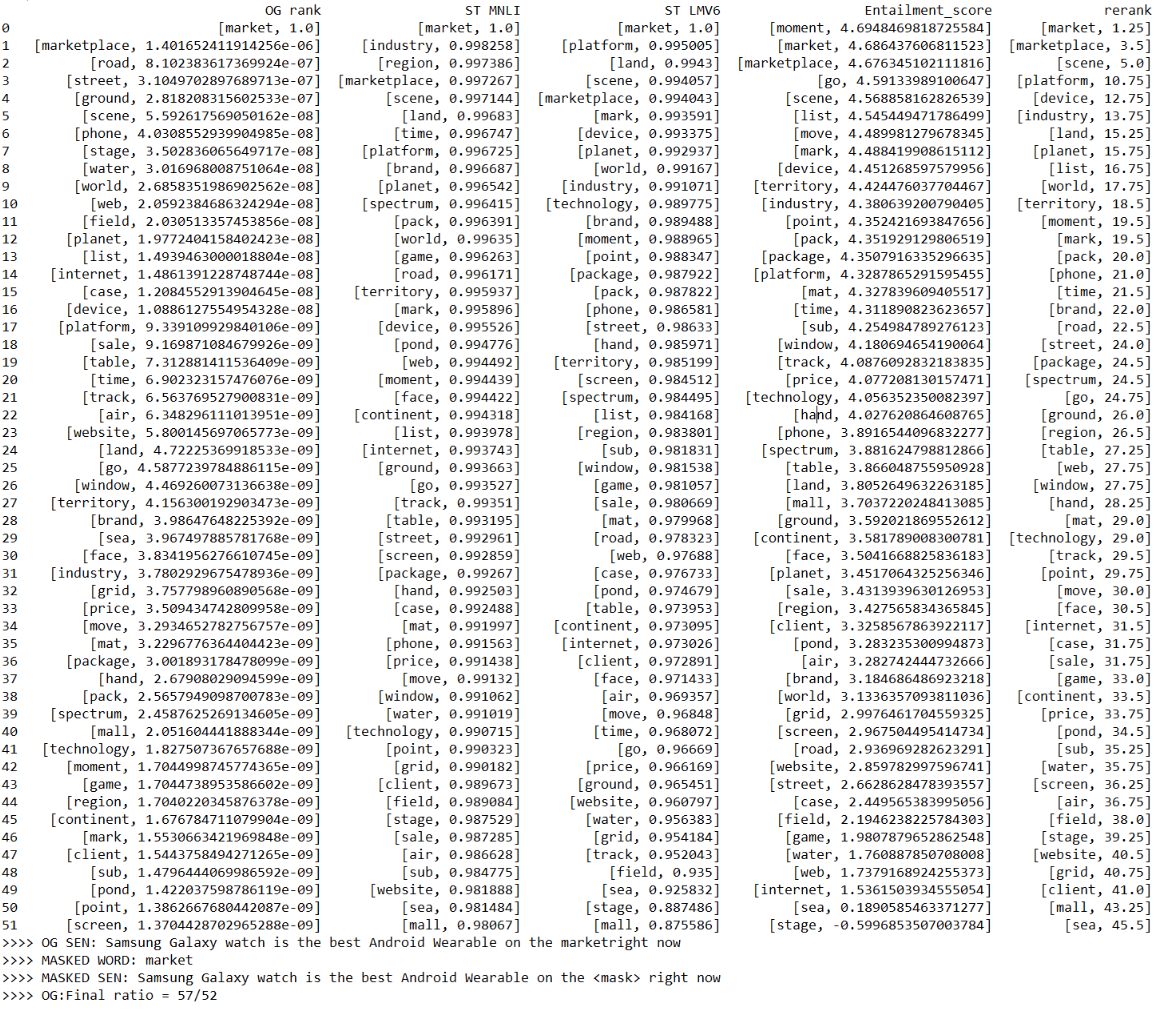
\includegraphics[width=15cm]{./img/chp4/ccr.png}}
\caption{consensus ranking}\label{fig:consensus ranking}
\end{figure}
Considers the above table to see the effect of consensus ranking. The first column shows raw output candidates and their ranking. Notice that some low-quality candidates are being placed very high on the list for instance “website” ranked 8th/51, “water” ranked 7th/51, “street” ranked 3th/51. 

The context is “Samsung Galaxy watch is the best Android Wearable on the market right now” where the word market is replaced with <mask>. 

According to the given sentence, none of the stated words should be ranked at the current position because they are totally irrelevant and do not preserve the meaning of the original sentence at all.



In consensus ranking, each judge (model) ranks the candidates independently, except the \verb/Entailment_score/ which uses the score from ST MNLI as a base. Those low-quality words have been pushed down the rank (2nd-4th column) because they received a lower score. Thus when aggregated (last column), the final output represents a better overall ranking quality. Despite averaging the position across all rankings, in some contexts, the judges may fail to capture the potential candidates which leads to some appropriate substitutions being ranked lower.


It should be noted that most of the scores from ST MNLI and ST LMV6 are almost 1 because in our project, both sentences are treated as highly similar by the model. 

To elaborate;
\begin{itemize}
\item Samsung Galaxy watch is the best Android Wearable on the market right now
\item Samsung Galaxy watch is the best Android Wearable on the marketplace right now
\item Samsung Galaxy watch is the best Android Wearable on the website right now
\item Samsung Galaxy watch is the best Android Wearable on the industry right now
\item Samsung Galaxy watch is the best Android Wearable on the water right now
\end{itemize}
The only difference between the original sentence and the rest is the target word which explains why the majority of candidates received a score beyond 0.9.

\subsection{Out-of-the-box model vs finetuned model}
Overall, the finetuned model shows no significant improvement over the original, most of the predicted candidates are comparable, but with less variety and correctness. 


\begin{tabular}{lll}
\hline
\textbf{sentence} &
  \textbf{base model (rerank)} &
  \textbf{custom model (rerank)} \\ \hline
\begin{tabular}[c]{@{}l@{}}The sunset painted the sky \\ with vibrant colors. (vibrant)\end{tabular} &
  \begin{tabular}[c]{@{}l@{}}vibrant, vivid, colorful, \\ colourful, lively, bright, \\ vividly, lush, brilliant, \\ dynamic, flashy\end{tabular} &
  \begin{tabular}[c]{@{}l@{}}vibrant, vivid, colorful, \\ beautiful, rich, diverse, \\ different, lush, many, \\ lively, new\end{tabular} \\ \hline
\begin{tabular}[c]{@{}l@{}}The study findings indicate a strong \\ correlation between two key variables. (strong)\end{tabular} &
  \begin{tabular}[c]{@{}l@{}}strong, strongly, robust, \\ powerful, substantial, high, \\ large, vigorious, close, good, \\ strict\end{tabular} &
  \begin{tabular}[c]{@{}l@{}}strong, strongly,sharp, \\ large, high, powerful, \\ close, heavy, big, good, \\ deep\end{tabular} \\ \hline
\begin{tabular}[c]{@{}l@{}}Cutting-edge research in the field is published \\ by the prestigious academic journal. (prestigious)\end{tabular} &
  \begin{tabular}[c]{@{}l@{}}prestigious, foremost, prominent, \\ reputable, respectable, crucial, \\ elite, esteemed, important, \\ fashionable, distinguished\end{tabular} &
  \begin{tabular}[c]{@{}l@{}}prestigious, top, foremost, \\ prominent, major, premier, \\ main, classical, elite, small, \\ popular\end{tabular} \\ \hline
\end{tabular}




\subsection{Human judgment}

The goal of this metric is to verify the proportion of candidates considered good substitution using human feedback. The candidates presented to the annotator only include the top 15 words of the final aggregated output. This experiment does not involve ranking each candidate, the annotator only has two choices, to keep or to delete to word.

\textbf{Setting:}\\
Two annotators were given the original sentence, masked sentence, target masked word, and a list of final aggregated candidates. The following instruction was given:
\\\\
INSTRUCTION:
“Evaluate the substitution candidate by deleting irrelevant or inappropriate candidates from the list.
The candidates will replace <mask> position in the given sentence and it should preserve the semantics of the original sentence. Thanks”
\\\\
Both annotators are our colleagues with an English proficiency level of C1 (advanced level) according to the Common European Framework of Reference for Languages (CEFR). 
The Council of Europe describes C1 fluency as follows:
“Can understand a wide range of demanding, longer texts, and recognize implicit meaning. Can express him/herself fluently and spontaneously without much obvious searching for expressions. Can use language flexibly and effectively for social, academic and professional purposes. Can produce clear, well-structured, detailed text on complex subjects, showing controlled use of organisational patterns, connectors and cohesive devices.”\cite{q} 
\\
The result is represented as follows:
\begin{itemize}

\item OG SEN: original sentence without mask
\item MASKED WORD: target word to mask
\item MASKED SEN: sentence replaced the target word with <mask> token


\item Final: the aggregated final ranking using consensus scheme
\item Anotator Overlap: words that both annotators selected as appropriate substitutions. This indicates 100 percent agreement between 2 judges.
\item Percent Usable: proportion of words that appear in Annotator Overlap that are also in Final. Assuming an ideal candidate is the one appears in Annotator Overlap percent 
\item Usable metric indicates how many words in the top 15 are considered a good substitution based on human judgment. 
\end{itemize}
% Please add the following required packages to your document preamble:
% \usepackage[table,xcdraw]{xcolor}
% If you use beamer only pass "xcolor=table" option, i.e. \documentclass[xcolor=table]{beamer}

\begin{tabular}{lllll}
\hline

\multicolumn{5}{l}{\begin{tabular}[c]{@{}l@{}}\textgreater{}\textgreater{}\textgreater{}\textgreater OG SEN: The punishment given to the rich people is unsatisfactory to the victim's family.\\ \textgreater{}\textgreater{}\textgreater{}\textgreater MASKED WORD: people\\ \textgreater{}\textgreater{}\textgreater{}\textgreater MASKED SEN: The punishment given to the rich \textless{}mask\textgreater is unsatisfactory to the victim's family.\end{tabular}} \\ \hline
Final &
  Annotator 1 &
  Annotator 2 &
  Annotator Overlap &
  \% Usable \\ \hline

\begin{tabular}[c]{@{}l@{}}{[}'people', 'folks',\\ 'ones',  'persons',\\ 'individuals',  'classes',\\ 'men', 'citizens', \\ 'things', 'criminals',\\ 'subjects', 'groups',\\ 'leaders', 'masses', \\'guys'{]}\end{tabular} &
  \begin{tabular}[c]{@{}l@{}}{[}'people', 'folks',\\ 'ones',  'persons',\\ 'individuals',  'classes', \\'men', 'citizens',\\ 'criminals', 'subjects', \\ 'leaders', 'guys'{]}\end{tabular} &
  \begin{tabular}[c]{@{}l@{}}{[}'people', 'folks',\\ 'ones',  'individuals', \\'classes',  'men',\\ 'citizens', 'criminals',\\  'subjects'{]}\end{tabular} &
  \begin{tabular}[c]{@{}l@{}}\{'subjects', \\'individuals', \\ 'folks', 'criminals',\\ 'classes',  'men', \\'citizens', 'ones',\\  'people'\}\end{tabular} &
  60 \\ \hline

\multicolumn{5}{l}{\begin{tabular}[c]{@{}l@{}}\textgreater{}\textgreater{}\textgreater{}\textgreater OG SEN: During the lecture, the professor explained the concept with clarity.\\ \textgreater{}\textgreater{}\textgreater{}\textgreater MASKED WORD: concept\\ \textgreater{}\textgreater{}\textgreater{}\textgreater MASKED SEN: During the lecture, the professor explained the \textless{}mask\textgreater with clarity.\end{tabular}} \\ \hline
\begin{tabular}[c]{@{}l@{}}{[}'concept', 'idea', \\'notion', 'premise',\\ 'topic', 'principle', \\ 'thing', 'point', \\'subject','proposition', \\'process', \\ 'information',\\ 'phenomenon', \\ 'thought', 'term'{]}\end{tabular} &
  \begin{tabular}[c]{@{}l@{}}{[}'concept', 'idea', \\'notion', \\ 'premise', 'topic', \\'principle', \\ 'point', 'subject', \\'process',\\  'information', \\ 'phenomenon', 'term'{]}\end{tabular} &
  \begin{tabular}[c]{@{}l@{}}{[}'concept', 'idea',\\ 'notion',  'topic',\\ 'point', 'subject',\\  'term'{]}\end{tabular} &
  \begin{tabular}[c]{@{}l@{}}\{'idea', 'point', 'topic',\\  'notion', 'term',\\ 'subject', 'concept'\}\end{tabular} &
  46.66 \\ \hline
\end{tabular}\\\\
The full data contain 25 sentences with the percent usable ranging from 13.33 percent (2/15 overlap) up to 73.33 percent (11/15 overlap), with an average overlap of 39.46 percent


\section{Comparing to the existing product}
Our approach is able to uncover hidden synonyms that are otherwise missed by Grammarly, for instance, the word “strong” in “The study findings indicate a strong correlation between two key variables.”, candidates like “high” and “close” are a good replacement in the sentence “The study findings indicate a strong correlation between two key variables.”, but may not be counted as a synonym without taking into account the surrounding context. This is also true for “criminals” as it is not a synonym of the word “people” if we do not consider its contextual information. However, “criminal” is a fairly suitable substitution for “The punishment given to the rich people is unsatisfactory to the victim's family”
\\\\
% Please add the following required packages to your document preamble:
% \usepackage[table,xcdraw]{xcolor}
% If you use beamer only pass "xcolor=table" option, i.e. \documentclass[xcolor=table]{beamer}

\begin{tabular}{lll}
\hline
\textbf{sentence} &
  \textbf{Our work} &
  \textbf{Grammarly} \\ \hline
\begin{tabular}[c]{@{}l@{}}The punishment given to the rich people \\ is unsatisfactory to the victim's family. \\(people)\end{tabular} &
  \begin{tabular}[c]{@{}l@{}}people, persons, ones, things, \\ men, folks, criminals, families, \\ guys, individuals, citizens\end{tabular} &
  \begin{tabular}[c]{@{}l@{}}individuals, somebody, \\someones\end{tabular} \\ \hline
\begin{tabular}[c]{@{}l@{}}During the lecture, the professor explained \\ the concept with clarity.\\ (concept)\end{tabular} &
  \begin{tabular}[c]{@{}l@{}}{[}'concept', 'idea', 'notion', \\'premise',  'topic', 'principle',\\ 'thing', 'point', \\ 'subject','proposition', 'process',\\  'information', 'phenomenon', \\ 'thought', 'term'{]}\end{tabular} &
  \begin{tabular}[c]{@{}l@{}}idea, picture, image, \\notion, vision \end{tabular}\\ \hline
\begin{tabular}[c]{@{}l@{}}The study findings indicate a strong \\ correlation between two key variables.\\ (strong)\end{tabular} &
  \begin{tabular}[c]{@{}l@{}}strong, strongly, robust, powerful, \\ substantial, high, large, vigorious,\\  close, good, strict\end{tabular} &
  \begin{tabular}[c]{@{}l@{}}robust, healthy, vital, \\vigorious, \\ substantial, firm, decisive\end{tabular} \\ \hline
\begin{tabular}[c]{@{}l@{}}Cutting-edge research in the field is published \\ by the prestigious academic journal.\\ (prestigious)\end{tabular} &
  \begin{tabular}[c]{@{}l@{}}prestigious, foremost, prominent, \\ reputable, respectable, crucial, \\ elite, esteemed, important, \\ fashionable, distinguished\end{tabular} &
  N/A \\ \hline
\end{tabular}

\section{User testing result}
Excluding a basic testing strategy, in order to see an actual response of the application’s performance and if it accomplished users need. We have given a chance to a total of 14 representatives to do hands-on testing of our application. By letting them test how to use the program with some advice from us as developers. And giving them a user survey of our application using Google Form, to collect responses if they like the features or not. \\

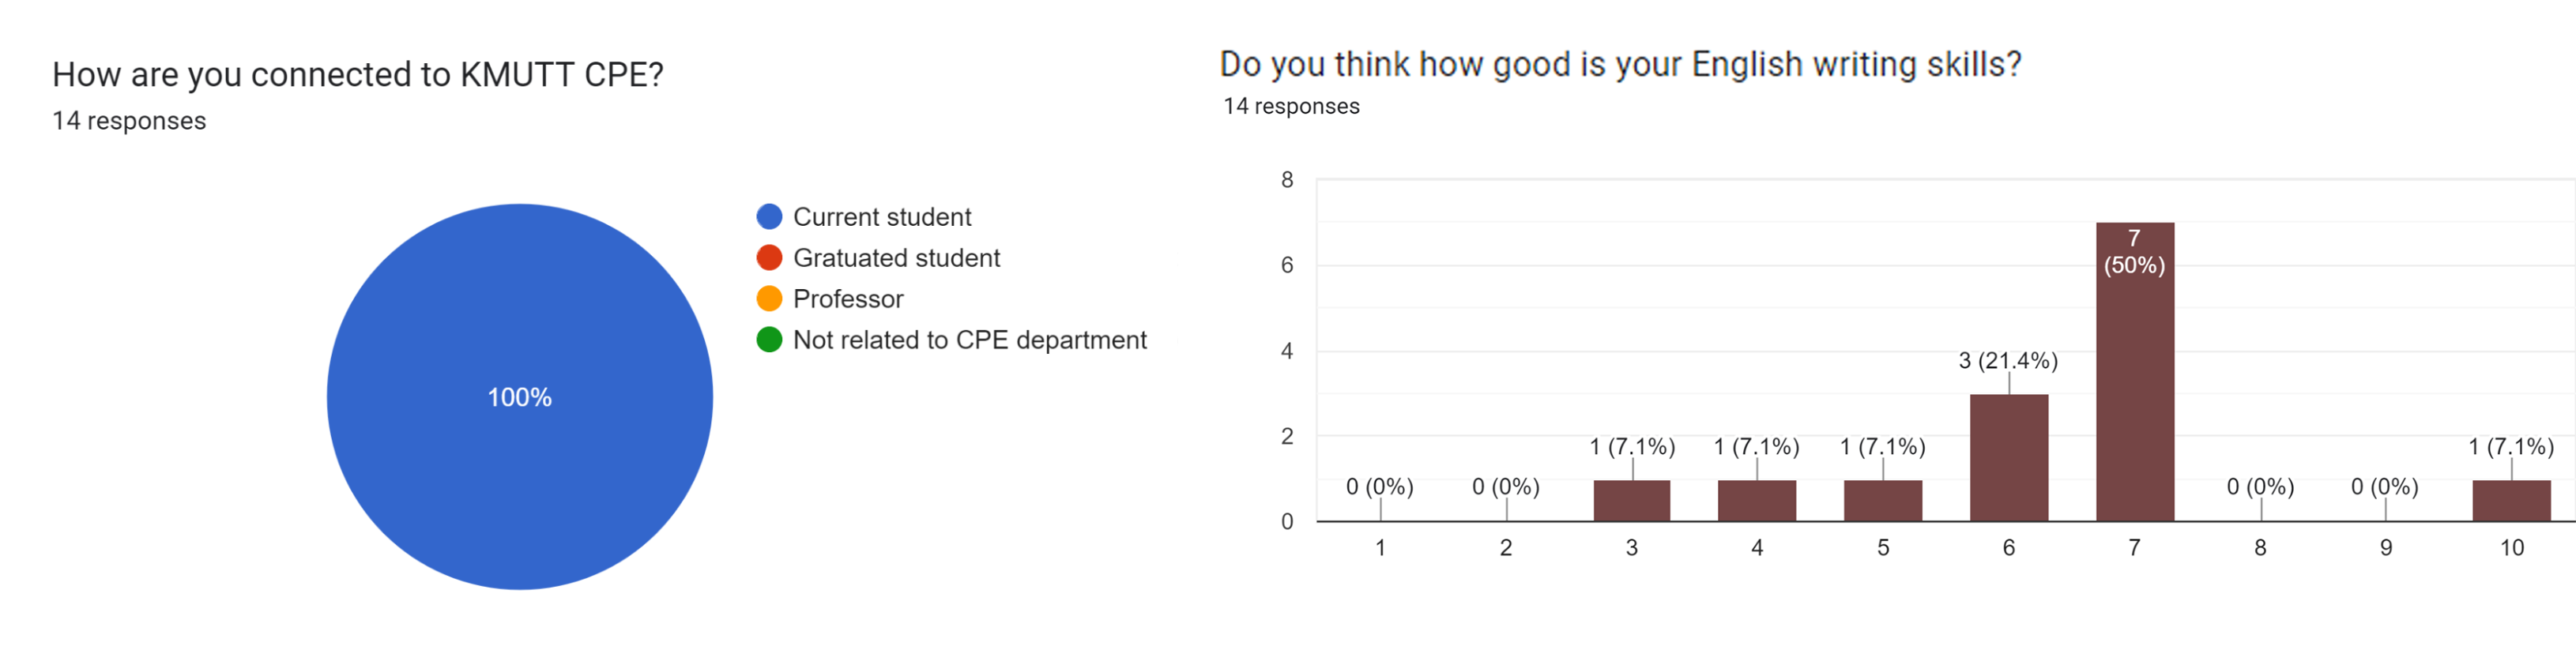
\includegraphics[width=15cm]{./img/chp4/q-info.png}\\

The full form of survey is located at \ref{survey}. According to the responses, all of responses are from current students of KMUTT CPE with half of them feeling quite confident with their writing skills. And the results of the survey data are shown below.

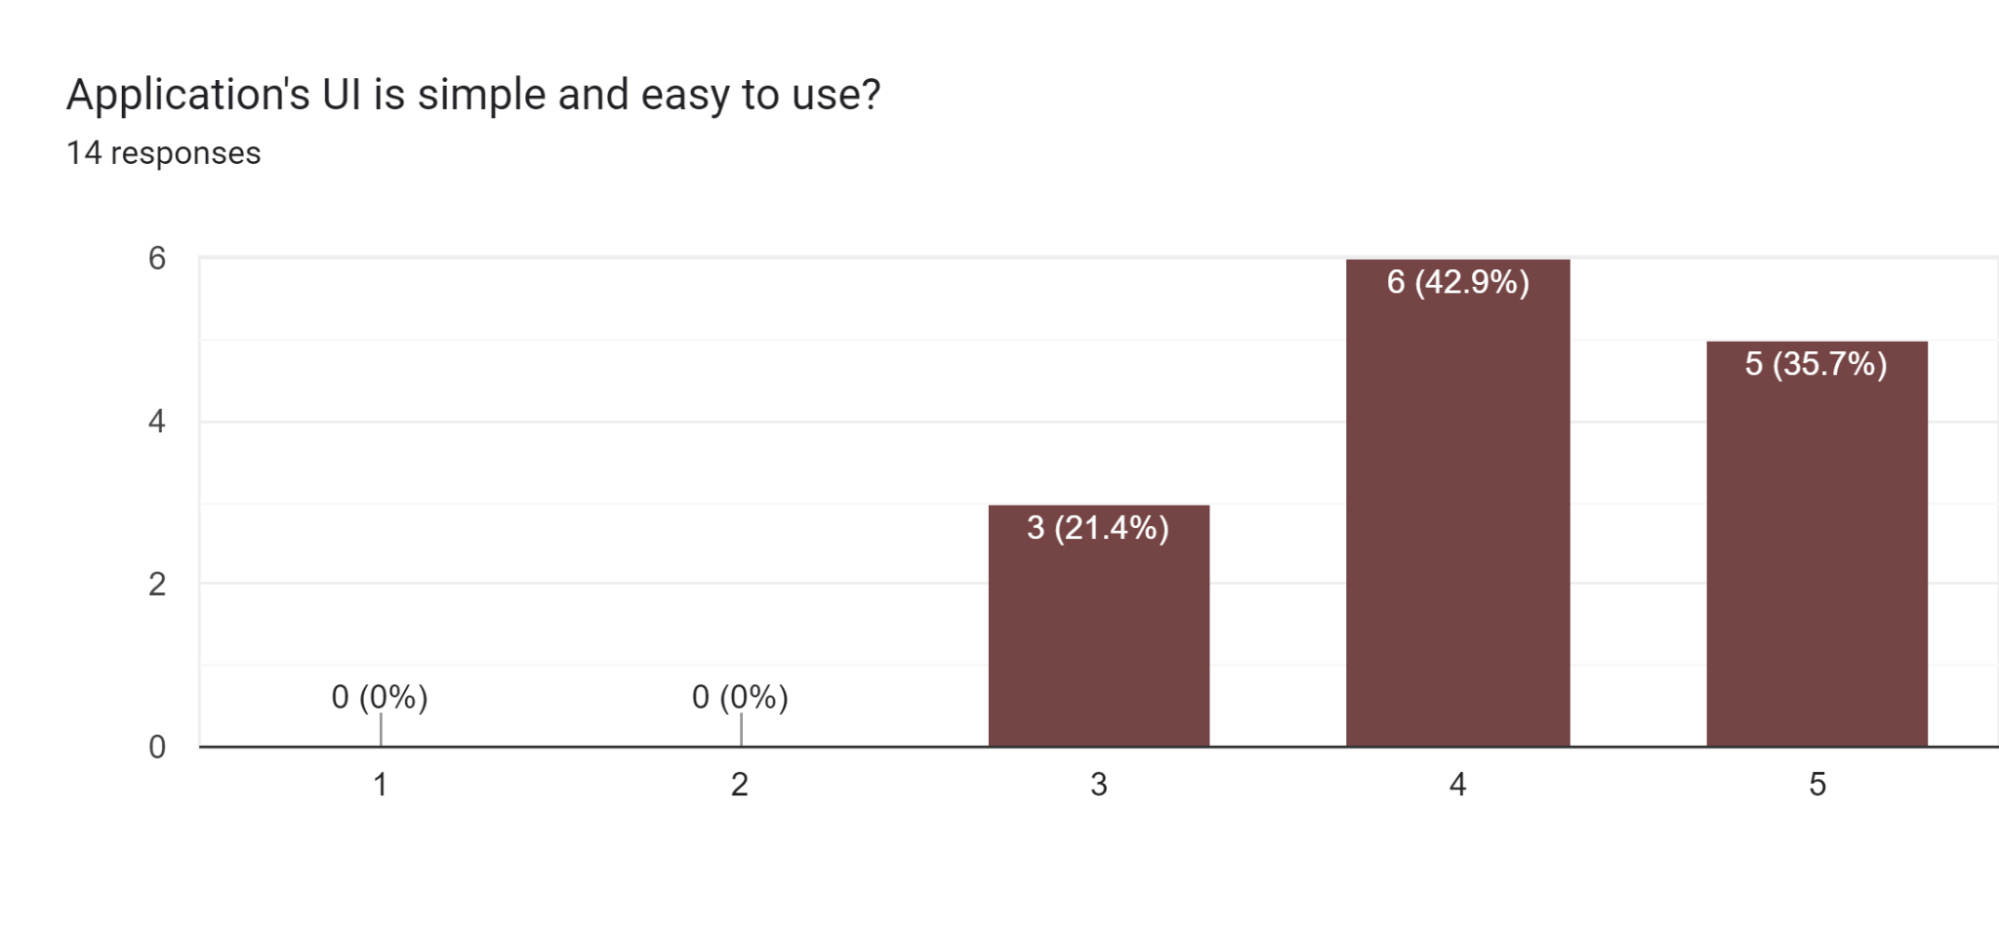
\includegraphics[width=15cm]{./img/chp4/q-use1.png}
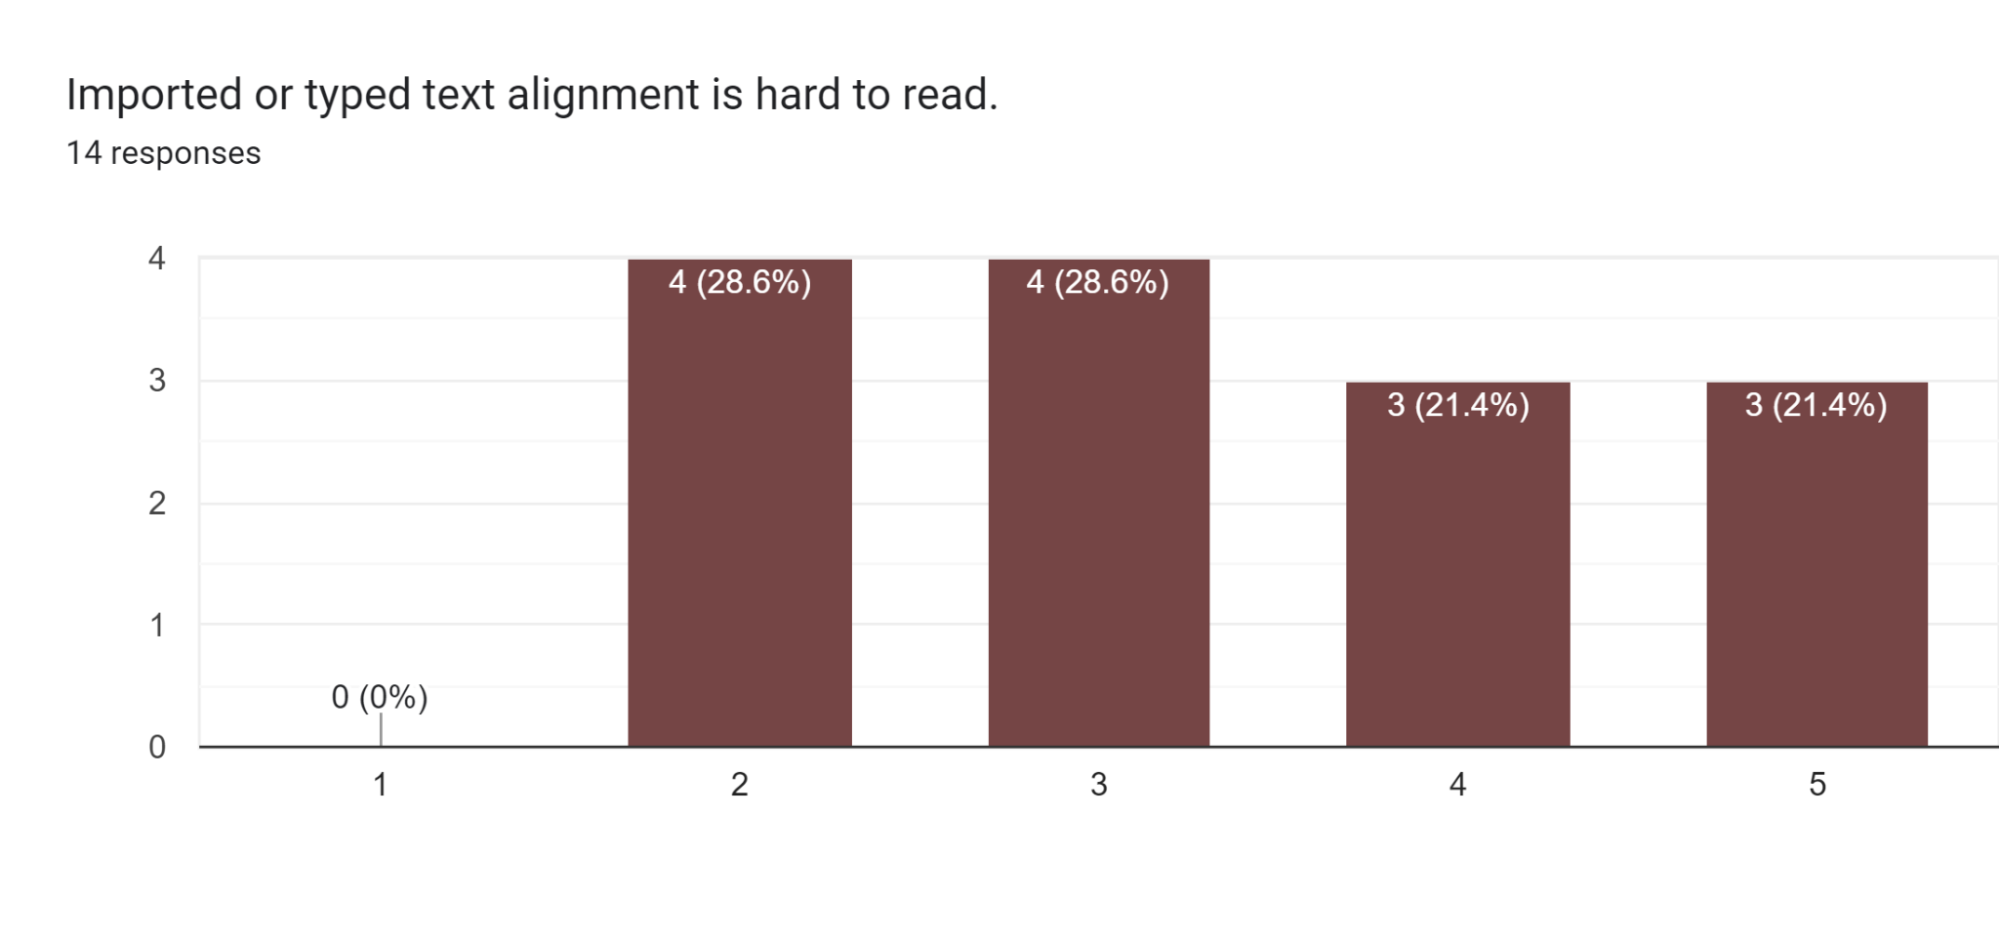
\includegraphics[width=15cm]{./img/chp4/q-use2.png}
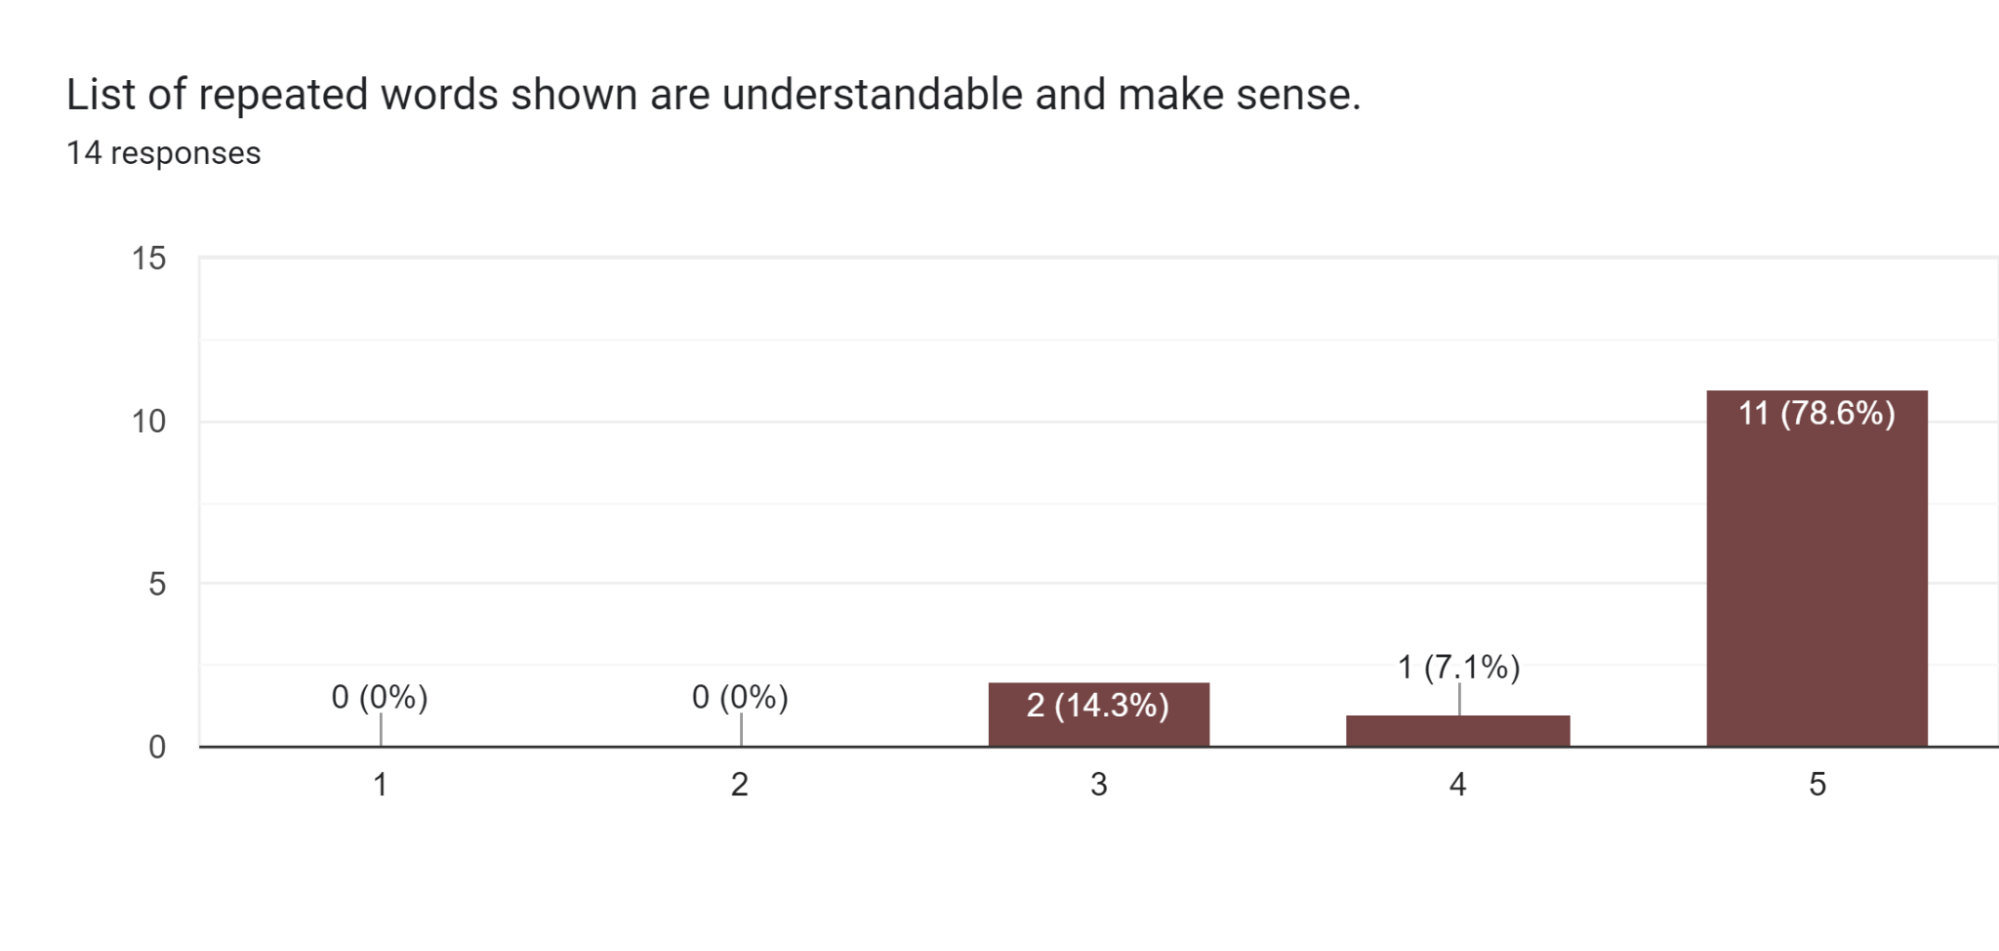
\includegraphics[width=15cm]{./img/chp4/q-use3.png}
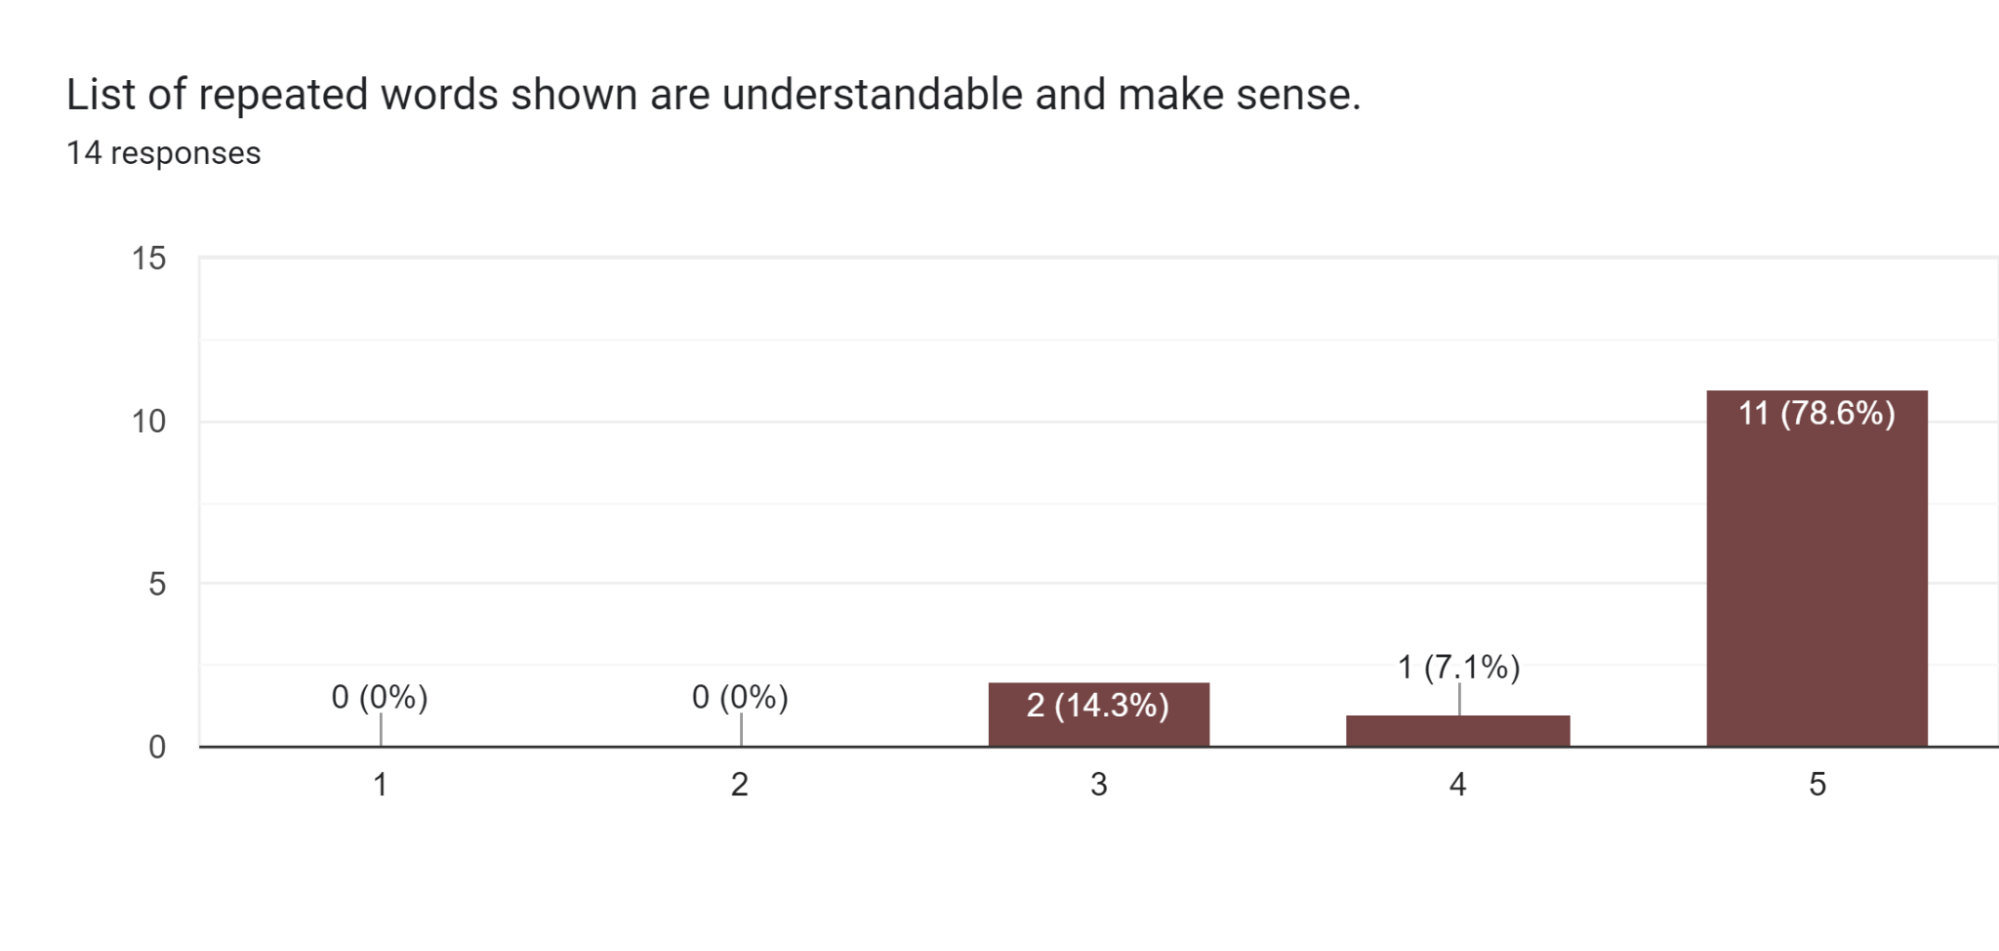
\includegraphics[width=15cm]{./img/chp4/q-use3.png}
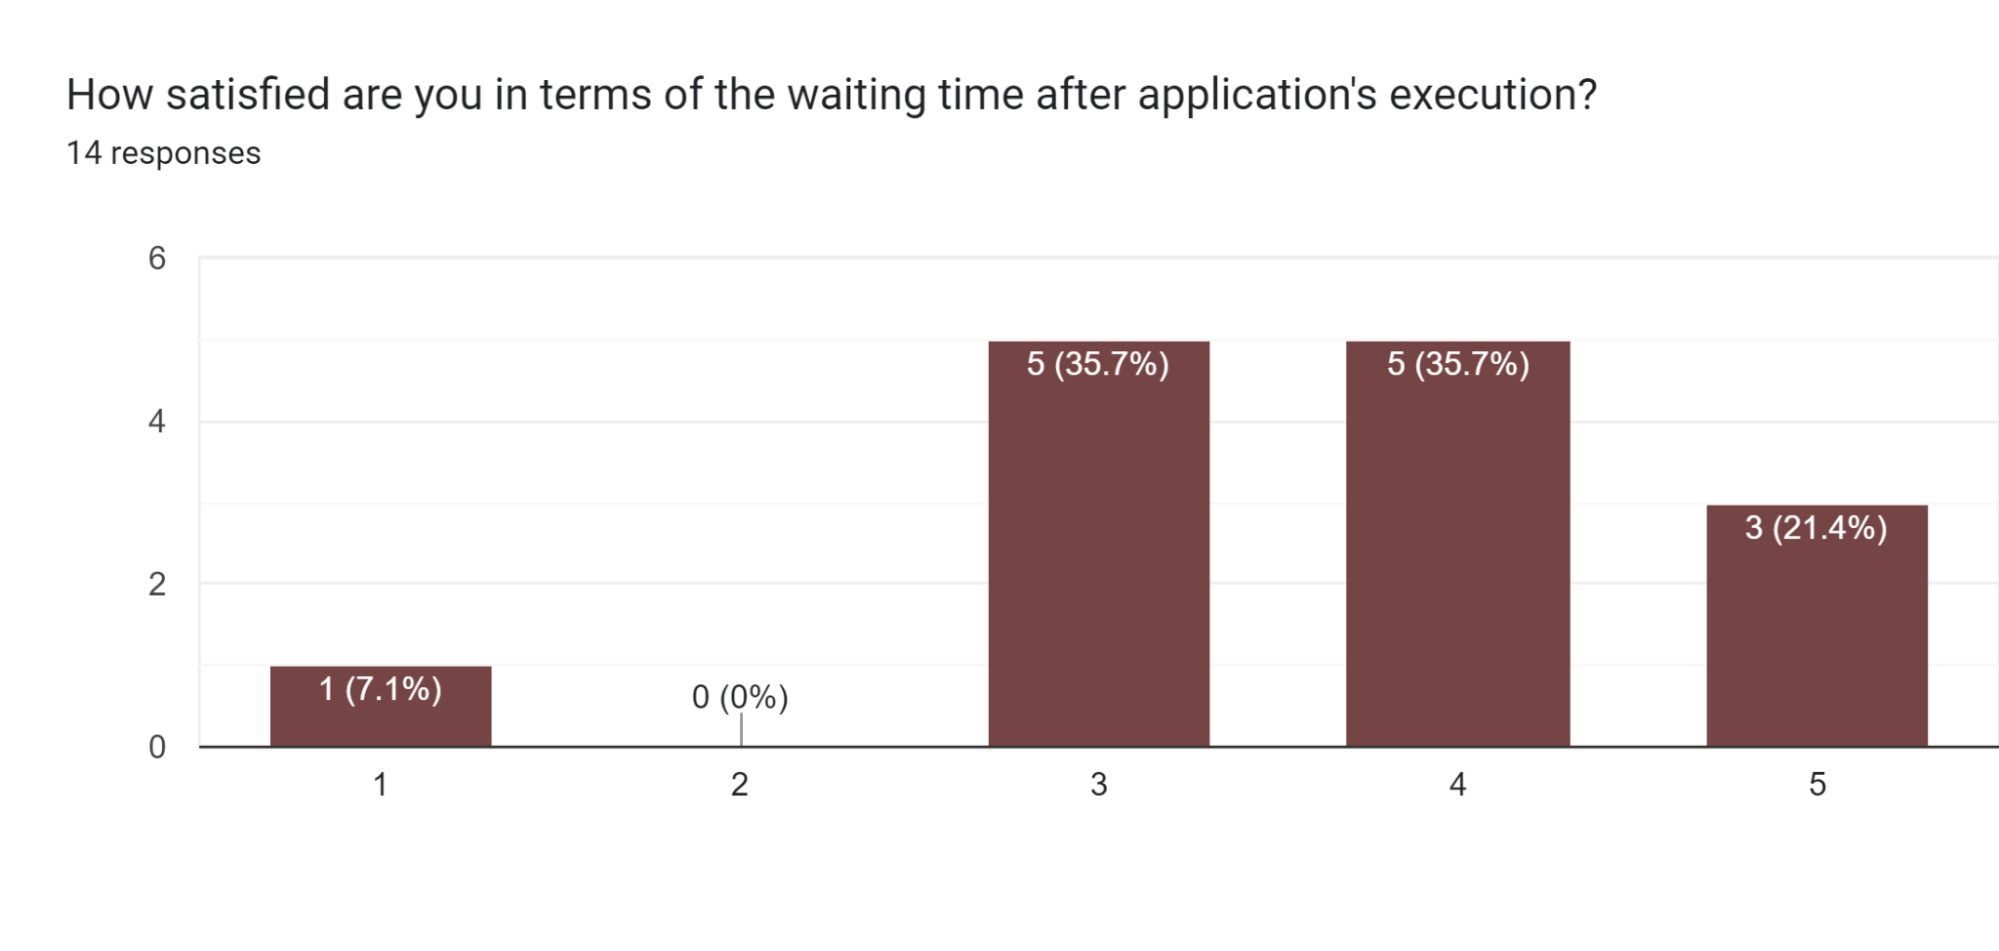
\includegraphics[width=15cm]{./img/chp4/q-use5.png}
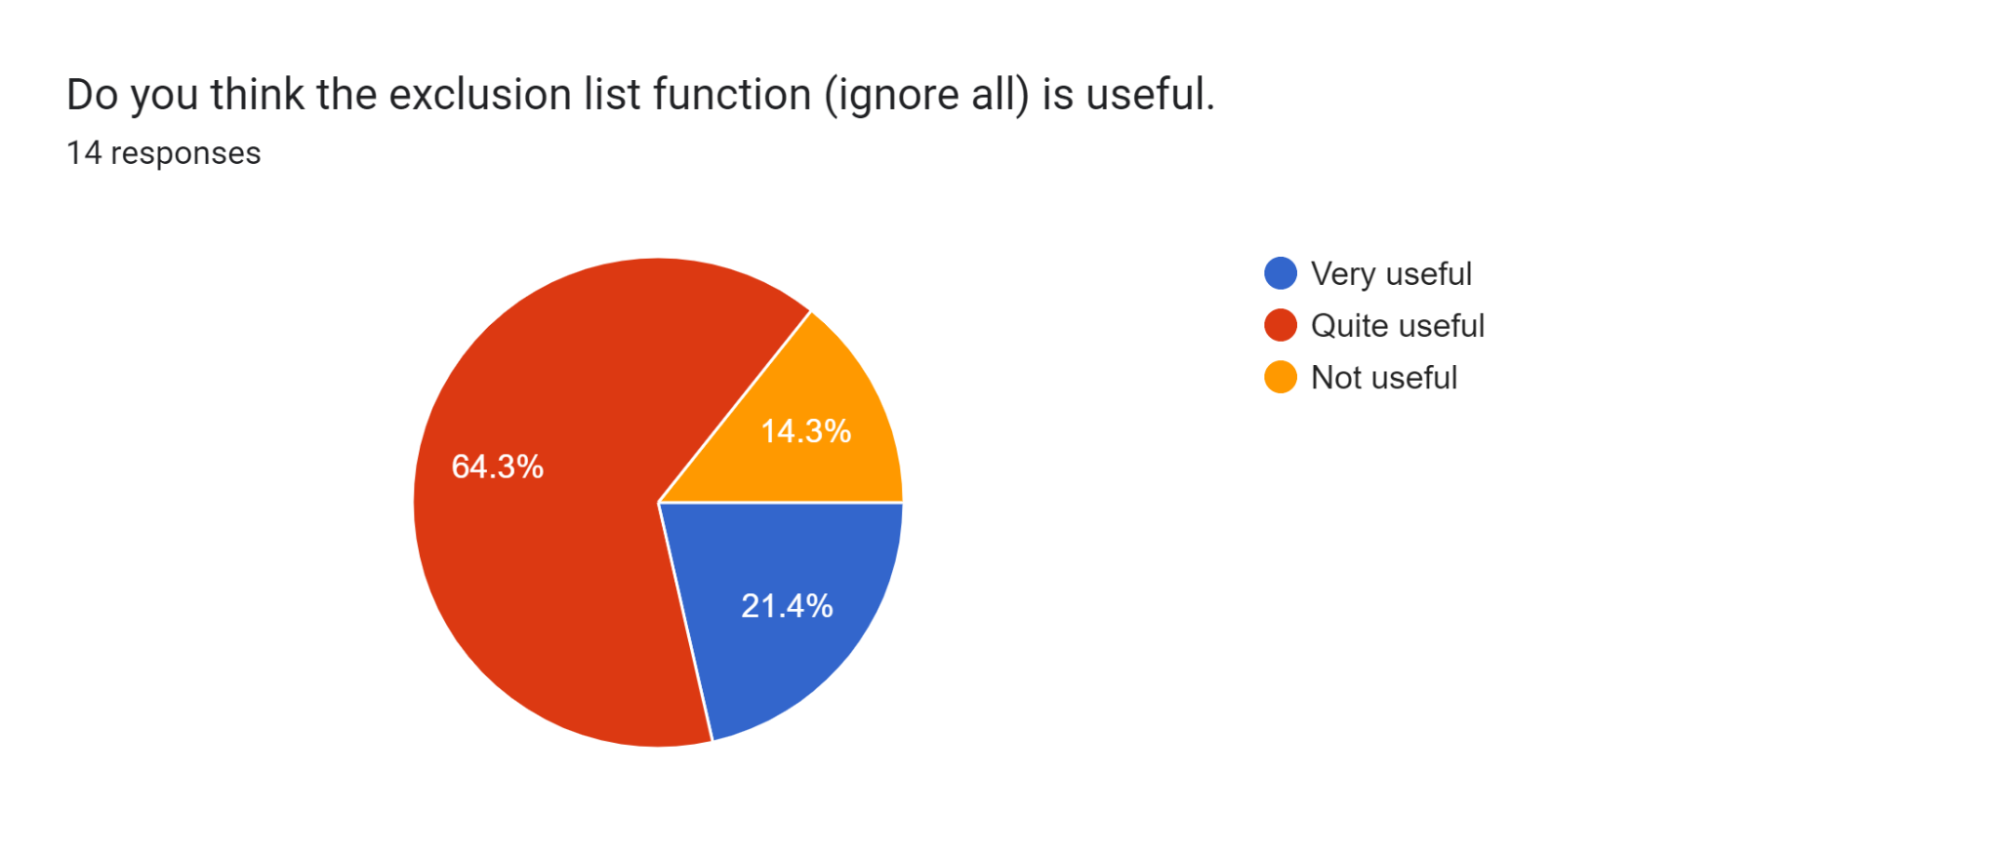
\includegraphics[width=15cm]{./img/chp4/q-use6.png}
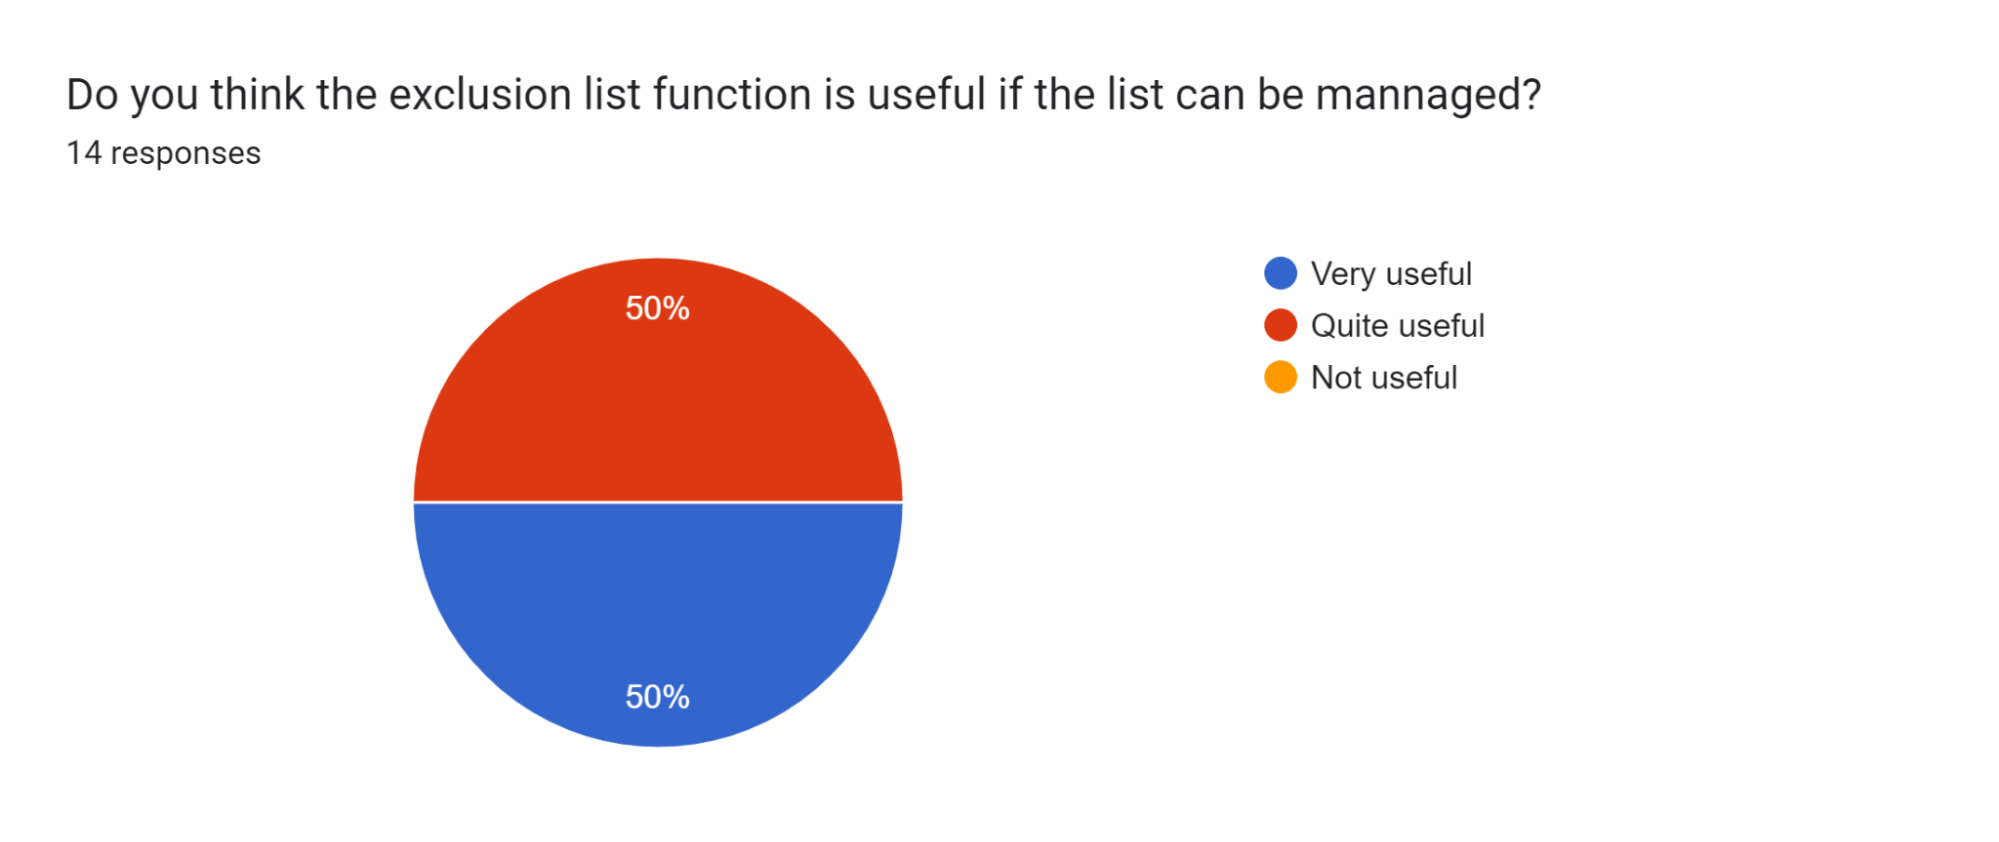
\includegraphics[width=15cm]{./img/chp4/q-use7.png}
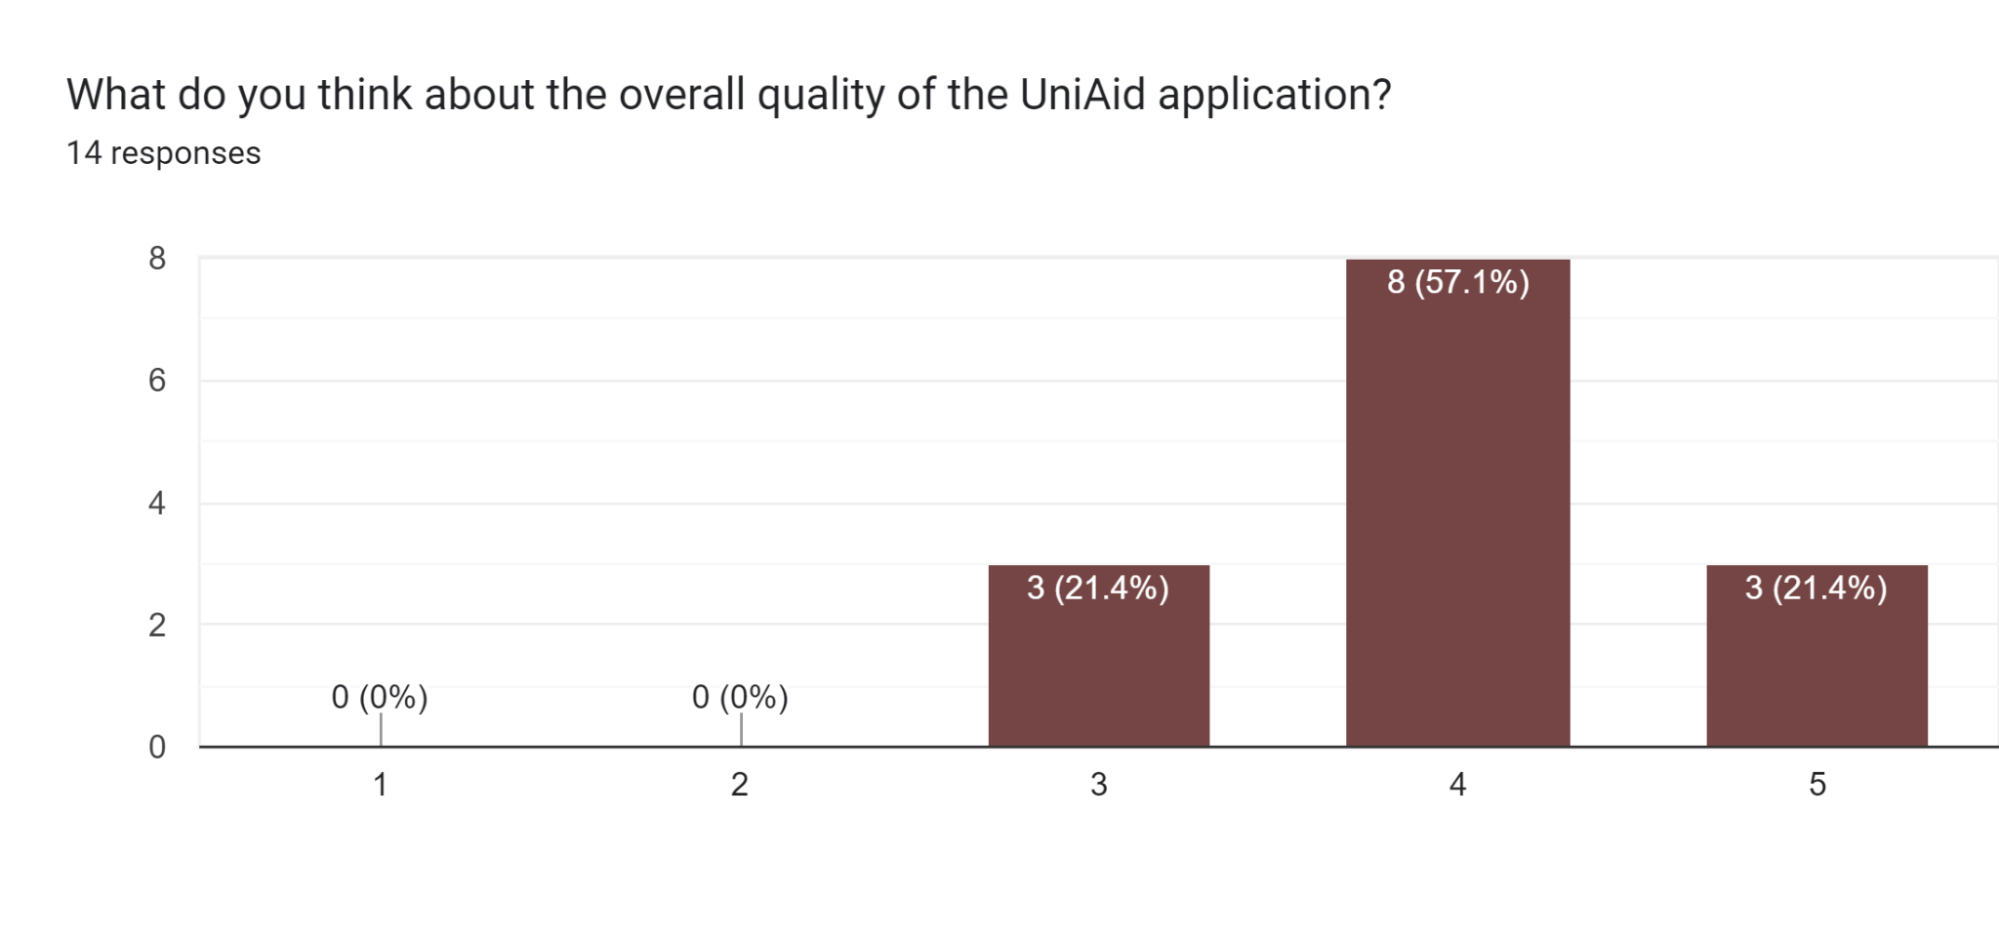
\includegraphics[width=15cm]{./img/chp4/q-use8.png}
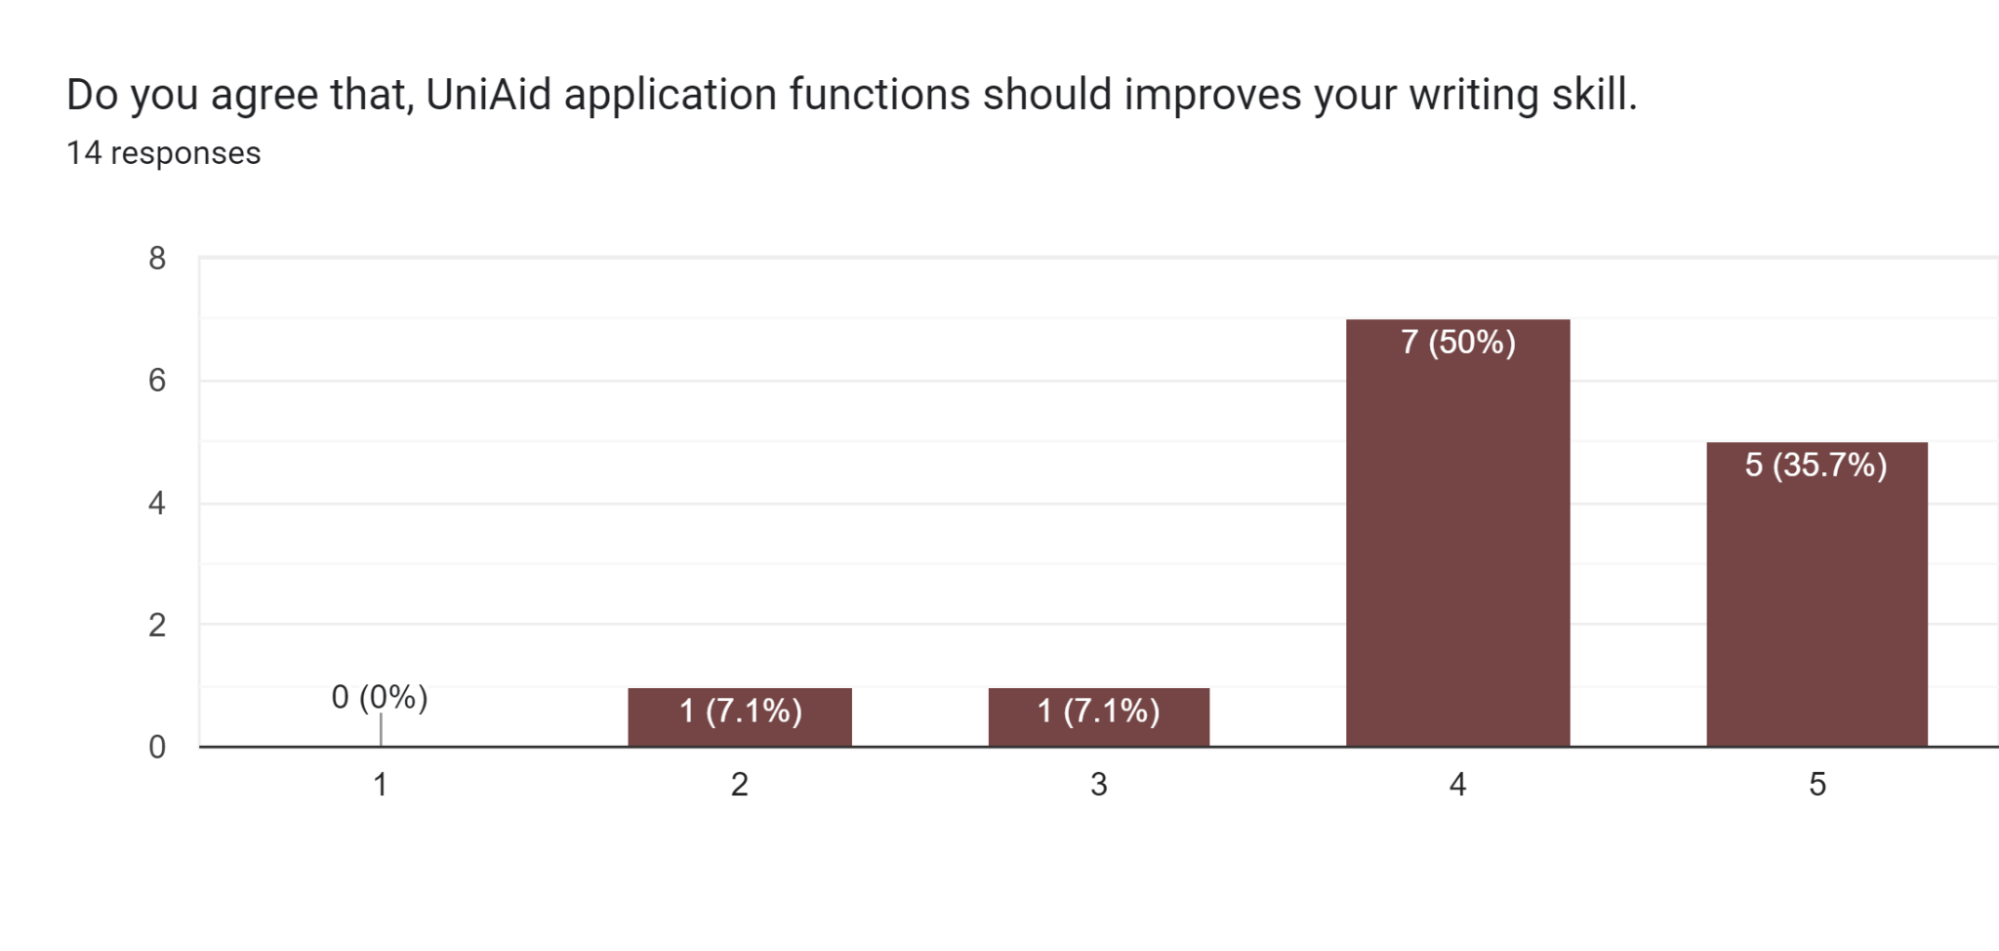
\includegraphics[width=15cm]{./img/chp4/q-use9.png}

To conclude the responses we got, they were mostly comfortable with the application's UI arrangement. Most test users agree that the repeated word shown is accurate and makes sense to show. Also the list of suggested words looks possible for replacement. \\

On the other hand, More than half of them are not feeling ok with the text input shown in the text box, since it’s hard to read or match the position with the original text file. Some of the test users also are not feeling good with the speed of execution which is especially at the suggestion part. And they also think that the exclusion list function is still not that useful right now. But if it has an option to manage or remove words from the exclusion list. All of the test users think that it should have some uses at least. As the overall responses results, most of test users think that the quality of the application is good, and has the potential of helping them in their writing.


\chapter{Conclusion}

In conclusion, our senior project aimed to develop a program that addresses the common challenge of repetitive usage of words often found in non-native writers. We offered a stand alone desktop application with a graphical user interface capable of detecting overused words from document files or user-typed text. Through natural language processing knowledge, we were able to detect and highlight relevant repetitions presented in the document. By leveraging the Transformer Fill Mask approach, our program was able to produce a wide variety of substitutions based on context including suitable words that may be missed by the existing solutions.\\

Our approach is able to uncover hidden synonyms, for instance,  the model was able to automatically predict the word “high” and “close” as a replacement for the word “strong” in the context of “strong correlation between…”. This demonstrated that it is capable of capturing contextual information, gaining more coverage than other approaches.
With the help of machine learning, our detector can accurately distinguish between generic words and named entities, allowing it to give suggestions only for the words that matter. In addition to detecting overused words and suggesting alternatives, our program offers a visual representation by identifying and highlighting repetitive words within the text. This feature allows writers to easily identify areas that need improvement, enhancing their ability to address repetitive word usage effectively.\\



While our program successfully captures a wide range of indirect synonyms and achieves a greater coverage in vocabulary options compared to other non-contextual methods, it is important to acknowledge the accuracy issue present in the output. Due to the nature of the machine learning-based approach, the program often generates incorrect word substitutions, words with incorrect parts of speech, or suggests irrelevant words. These inaccuracies can impact the overall quality and effectiveness of the suggestions. To mitigate these accuracy issues, we have implemented multiple sanitization policies that filter out incorrect substitutions based on their linguistic attributes including part-of-speech filtering, antonym cleaning, and inflection cleaning. Moreover, a sentence concatenation technique is applied to keep the generated substitutions relevant to the original word. Additionally, a consensus ranking mechanism has been employed to adjust the ranking of the final suggestions by aggregating rankings from multiple judges. Prioritizing high-quality candidates that are better suited for a given sentence over those with lower relevance. \\

It is worth noting that, like any language processing tool, our program may still exhibit certain limitations. The nature of machine learning-based approaches can result in gender biases, reflecting the biases inherent in real-world language usage. Furthermore, limitations such as the inability of the end-user to continue working due to the lack of saving features, mean that they will need to open the file again every time. This also affect the unsaveed Exclusion list, means that user still can add a word to the exception list, but they're not able to gain those word back after they close the program. But surely that, this can be developed. Next, occasional connectivity issues with the Huggingface Hub API, preventing access to model repositories. Lastly, high resource utilization including processors and RAM due to the characteristic of the Transformer-based technique. The mentioned obstacle may affect the overall usability of the program in the real world.
Another challenge we encountered was the amount of computation required to finetune the Transformer model, leading to limited experimentation and unsatisfactory outcome.\\\\

Moving forward, further exploration and refinement are needed to improve the accuracy of the program's output. Incorporating a new technology such as a generative AI and large language model could potentially enhance the relevance and precision of the suggested alternatives.\\

In summary, our project provides a practical tool for writers to enhance the quality of their written work by detecting overused words and offering contextually appropriate alternative suggestions. By considering the surrounding context, our program offers a broader coverage and uncovers hidden synonyms that are otherwise missed by other tools. While limitations exist, we have implemented measures to improve accuracy, prioritizing more suitable alternatives and refining the output. With its visual highlighting feature, our program assists writers in identifying and addressing repetitive word usage effectively.



%%%%%%%%%%%%%%%%%%%%%%%%%%%%%%%%%%%%%%%%%%%%%%%%%%%%%%%%%%%%%%%
%%%%%%%%%%%%%%%%%%%% Conclusions %%%%%%%%%%%%%%%%%%%%%%%%%%%%%
%%%%%%%%%%%%%%%%%%%%%%%%%%%%%%%%%%%%%%%%%%%%%%%%%%%%%%%%%%%%%%%
%\chapter{Conclusions}
%
%This chapter is optional for proposal and progress reports but 
%is required for the final report.
%
%\section{Problems and Solutions}
%State your problems and how you fixed them.
%
%\section{Future Works}
%What could be done in the future to make your projects better.

%%%%%%%%%%%%%%%%%%%%%%%%%%%%%%%%%%%%%%%%%%%%%%%%%%%%%%%%%%%%%%%
%%%%%%%%%%%%%%%%%%%% Bibliography %%%%%%%%%%%%%%%%%%%%%%%%%%%%%
%%%%%%%%%%%%%%%%%%%%%%%%%%%%%%%%%%%%%%%%%%%%%%%%%%%%%%%%%%%%%%%

%%%% Comment this in your report to show only references you have
%%%% cited. Otherwise, all the references below will be shown.
%\nocite{*}
%% Use the kmutt.bst for bibtex bibliography style 
%% You must have cpe.bib and string.bib in your current directory.
%% You may go to file .bbl to manually edit the bib items.

\makeatletter
\g@addto@macro{\UrlBreaks}{\UrlOrds}
\makeatother

\bibliographystyle{kmutt}
\bibliography{string,cpe}

%%%%%%%%%%%%%%%%%%%%%%%%%%%%%%%%%%%%%%%%%%%%%%%%%%%%%%%%%%%%%%%
%%%%%%%%%%%%%%%%%%%%%%%% Appendix %%%%%%%%%%%%%%%%%%%%%%%%%%%%%
%%%%%%%%%%%%%%%%%%%%%%%%%%%%%%%%%%%%%%%%%%%%%%%%%%%%%%%%%%%%%%%
\appendix{Appendix}
\section{Final output vs Rerank}
\begin{figure}[!h]\centering
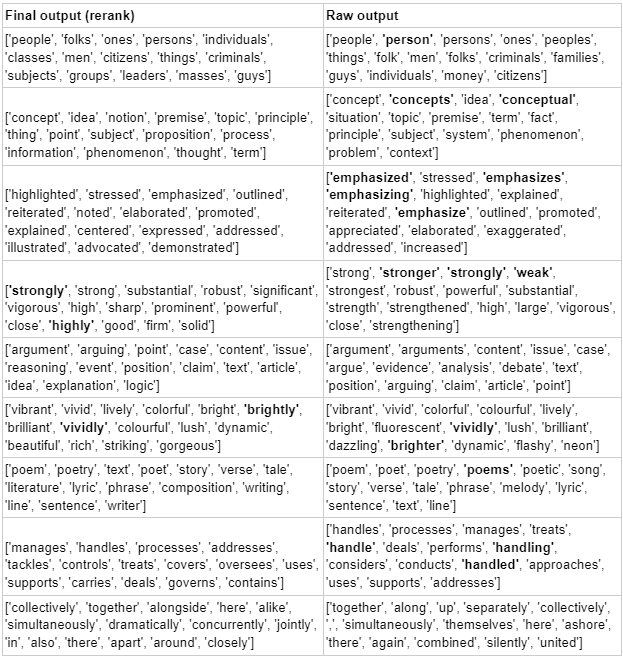
\includegraphics{./img/Appendix/FinalvsRerank.png}
\end{figure}

\newpage
\section{Base model vs custom model}
\begin{figure}[!h]\centering
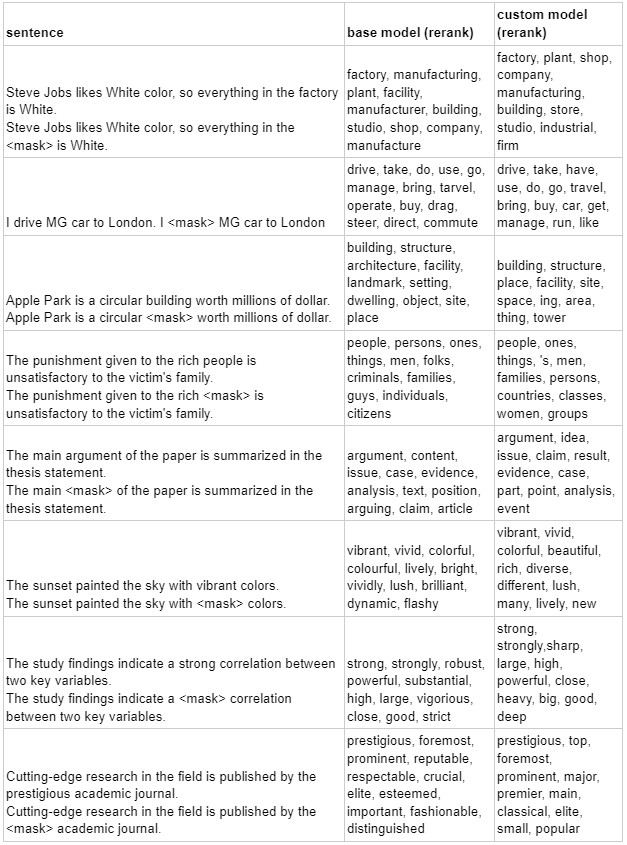
\includegraphics{./img/Appendix/BasevsCustom.png}
\end{figure}

\newpage
\section{Human evaluator}
\begin{figure}[!h]\centering
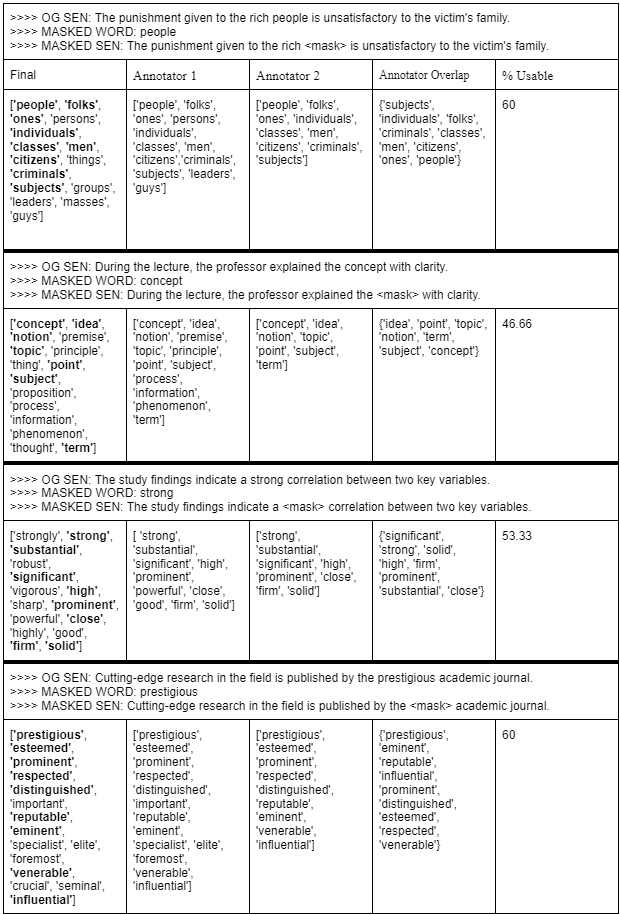
\includegraphics[width=15cm]{./img/Appendix/HumanEva.png}
\end{figure}

\newpage
\section{Compare to Grammarly}
\begin{figure}[!h]\centering
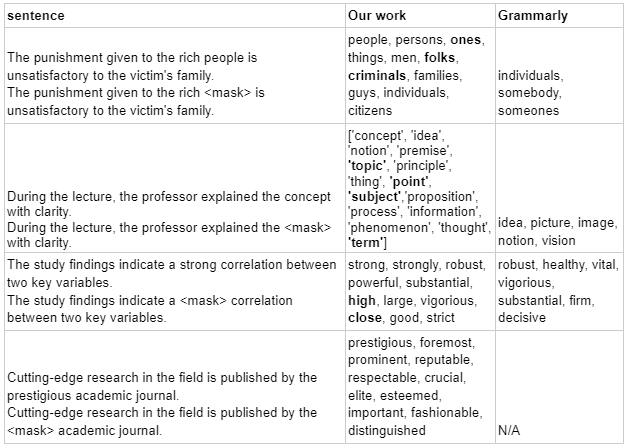
\includegraphics[width=15cm]{./img/Appendix/Grammarly.png}
\end{figure}

\newpage
\section{User test survey form(Google Form)\label{survey}} 

\includegraphics[width=15cm]{./img/Appendix/Survey-1-1.png}

\includegraphics[width=15cm]{./img/Appendix/Survey-1-2.png}
\includegraphics[width=15cm]{./img/Appendix/Survey-1-3.png}
\includegraphics[width=15cm]{./img/Appendix/Survey-2-1.png}
\includegraphics[width=15cm]{./img/Appendix/Survey-2-2.png}
\includegraphics[width=15cm]{./img/Appendix/Survey-2-3.png}
\includegraphics[width=15cm]{./img/Appendix/Survey-2-4.png}
\includegraphics[width=15cm]{./img/Appendix/Survey-2-5.png}
\includegraphics[width=15cm]{./img/Appendix/Survey-2-6.png}
\includegraphics[width=15cm]{./img/Appendix/Survey-2-7.png}
\includegraphics[width=15cm]{./img/Appendix/Survey-2-8.png}
\includegraphics[width=15cm]{./img/Appendix/Survey-2-9.png}


%%%%%%%%%%%%%%%%%%%%%%%%%%%%%%%%%%%%%%%%%%%%%%%%%%%%%%%%%%
%%%%%%%%%%%%%%% The 2nd appendix %%%%%%%%%%%%%%%%%%%%%%%%%%
%%%%%%%%%%%%%%%%%%%%%%%%%%%%%%%%%%%%%%%%%%%%%%%%%%%%%%%%%%
%\appendix{Second appendix title}
%\noindent{\large\bf Put appropriate topic here} \\

\end{document}
